\documentclass[10pt,openright1]{tudelft}


%\usepackage{bophook}

%
%\usepackage{thumby}
%\thumbySides{two}
%\thumbyTotalChapters{10}
%\thumbyPageHeight{795}
%\thumbyThumbWidth{42.5}
%\thumbyForeground{white}
%\thumbyBackground{black}
%\thumbyNumberFormat{\Huge\textbf{$chapter number}}
%\thumbySetup



% for debugging
% \usepackage{showkeys} % Shows all labels
% \usepackage{layouts}
% our text width is 369.0 pts = 12.967 cm

% for annotations in the WIP-version
\usepackage[]{todonotes}

% forcing figure placement
\usepackage{placeins}
% \FloatBarrier

% my preferred font, linux libertine
\usepackage{libertine}
\usepackage[T1]{fontenc}
%\usepackage[libertine]{newtxmath}

% more 
\usepackage{bbold}
\usepackage{enumitem}

% tables
\usepackage{tabu}
\usepackage{multirow}

%for using .eps
\usepackage{epstopdf}

% formatting the figure captions
\definecolor{ocre}{RGB}{77,99,104}
\usepackage[format=plain,font={sf,color=ocre},labelfont={bf,up}]{caption}
\DeclareCaptionLabelSeparator{bar}{ |}
\captionsetup{labelsep=bar}

% depth of the TOC
\setcounter{tocdepth}{4}

% style of the section headings
%\usepackage{titlesec}
%\titleformat{\section}{\sffamily\bfseries\Large}{\thesection}{1em}{}

% where to look for figures (also, each chapter has their own)
\graphicspath{{figures/}} % Relative path for figures

% some unxiversal commands that are handy
\include{commands}

\begin{document}

% Front matter
\frontmatter
\include{frontmatter}
\chapter{Summary}

Gaining precise control over quantum systems is crucial for applications in quantum information processing and quantum sensing and to perform experimental tests of quantum mechanics. The experiments presented in this thesis implement quantum measurements and real-time feedback protocols that can help to achieve these goals using single electron and nuclear spins in diamond. Spins associated with the Nitrogen Vacancy (NV) center in diamond recently emerged as an excellent testbed to demonstrate quantum effects and are a promising building block for future quantum technology.\\

The NV center is an atomic defect in the diamond lattice consisting of a substitutional nitrogen atom next to an empty lattice site. With its effective electron spin and nearby nuclear spins it forms a natural multi-qubit register with long-lived spin states that can be manipulated with magnetic resonance techniques. At temperatures below 10 K it displays spin-selective optical transitions that can be individually addressed and thereby provide an optical interface enabling high-fidelity single-shot readout and the generation of spin-photon entanglement.\\

In chapter 3 the fundamental trade-off between information gain and state disturbance associated with a quantum measurement is investigated. A variable strength measurement of the nuclear spin associated with the host nitrogen atom is implemented via an indirect measurement using the electron spin. The measurement strength can be tuned by varying the amount of entanglement between the two spins. To avoid dephasing of the nuclear spin, due to spin-flips of the electron spin during its readout, a dynamical-stop readout is used to perform a QND measurement of the electron spin. This enables sequential partial measurements that can manipulate the nuclear spin using only the backaction of quantum measurements combined with real-time feedback. \\

The electron spin can be used to sense static magnetic fields by performing repetitive Ramsey sequences. The experiments presented in chapter 4 address the open question whether adaptive measurements can out-perform non-adaptive protocols for sensing applications. An adaptive strategy is implemented where the readout basis is optimized in real-time using a Bayesian estimation based on previous measurement outcomes. The experiment shows that this adaptive protocol outperforms the best known non-adaptive protocol when overhead is taken into account.\\

The results in chapter 5 demonstrate the generation of measurement-based entanglement between two electron spins separated by 3 meters. By locally entangling each electron spin with a photon and performing a subsequent joint measurement of the photons, entanglement between the electron spins is heralded. The generated Bell-pair shared between remote locations is then used to unconditionally teleport the state of a nuclear spin in one diamond to the electron spin in the other diamond. To this end the nuclear spin is prepared in the state that is to be teleported followed by a local measurement of the electron and nuclear spin in the Bell-basis. This measurement projects the electron spin in the other diamond to the initial state of the nuclear spin up to a unitary operation that depends on the outcome of the Bell-state measurement. The original state is then recovered via a feed-forward operation. The fact that the protocol to prepare the remote Bell-pair is heralded and that the local Bell-state measurement can distinguish all four Bell-states, allows for unconditional teleportation. \\

The final two chapters of this thesis discuss the use of weakly coupled $^{13}$C spins as a quantum memory that is robust against optical excitation of the electron spin. The ability to store a quantum state in a quantum register while remotely connecting it to other registers enables the implementation of entanglement purification and quantum repeater protocols. A theoretical model is introduced to analyze the dephasing of a carbon spin during repetitive resets of the electron spin (which is required in the presented heralded entanglement protocol). This model is then tested experimentally in an isotopically purified diamond with a carbon spin that is relatively insensitive to perturbations induced by electron spin-flips owing to its low coupling strength (200 Hz). Although the observed dephasing is stronger than predicted by the model the results indicate that it is possible to store a quantum state in the $^{13}$C spin while optically exciting the electron spin.

\chapter{Samenvatting}

Het nauwkeurig controleren van quantum systemen is essentieel zowel voor toepassingen in quantum informatica en quantum sensoren als voor experimentele tests van de quantum mechanica. De experimenten die in dit proefschrift worden beschreven, introduceren quantum metingen en terugkoppeling protocollen met enkele spins in diamant om deze doelen te bereiken. Spins nabij het stikstof-holte (nitrogen-vacancy, NV) centrum in diamant zijn uiterst geschikt om quantum effecten te demonstreren en zijn een veelbelovende bouwsteen voor toekomstige quantum technologie. \\

Het NV centrum is een atomisch defect in het diamant rooster bestaande uit een stikstofatoom in plaats van een koolstofatoom en een ontbrekend koolstofatoom op een naburige roosterplek. Met zijn elektron spin en nabijgelegen kernspins vormt het NV centrum een quantum register bestaande uit spins met lange coherentietijden die gemanipuleerd kunnen worden met magnetische resonantie technieken. Bij temperaturen beneden de 10 K vertoont het NV centrum spin-selectieve optische transities die individueel aangeslagen kunnen worden. Op deze manier kan de electron spin zeer betrouwbaar worden geinitialiseerd, gemeten en verstrengeld met een foton. \\

In hoofdstuk 3 wordt de fundamentele balans tussen het verkrijgen van informatie en het verstoren van een quantum toestand die hoort bij een quantum meting onderzocht. Door de kernspin te meten via de elektron spin kan de sterkte van de meting gevarieerd worden. Hierbij bepaalt de mate van verstrengeling tussen de twee spins de meetsterkte. Een nieuw ontwikkelde QND meting van de elektron spin kan decoherentie van de kernspin tijdens de uitlezing van de elektron spin verminderen. Dankzij deze QND meting kunnen opeenvolgende gedeeltelijke metingen op de kernspin worden gedaan. Tot slot laten we zien dat de terugslag van opeenvolgende gedeeltelijke metingen gebruikt kan worden om de toestand van de kernspin te manipuleren door gebruik te maken van tergkoppeling.\\

De elektron spin kan worden gebruikt om statische magnetische velden te meten door opeenvolgende Ramsey sequenties uit te voeren. De experimenten die besproken worden in hoofdstuk 4 richten zich de open vraag of het gebruik van terugkoppeling kan helpen om een quantum sensor te verbeteren. In het gedemonstreerde protocol met terugkoppeling wordt de meetbasis van de elektron spin geoptimaliseerd door een Bayesiaanse schatting te maken van het magneetveld gebaseerd op de voorgaande meetuitkomsten. De experimenten tonen aan dat het gebruik van terugkoppeling voordelig is wanneer men de \textit{overhead} meerekent.\\

De resultaten in hoofdstuk 5 demonstreren dat twee elektronen spins in diamanten op een afstand van 3 meter met elkaar verstrengeld kunnen worden door middel van metingen. Door de individuele elektronen spins lokaal te verstrengelen met een foton en vervolgens de fotonen gezamenlijk te meten, worden de elektronen spins in een verstrengelde toestand geprojecteerd. Het resulterende Bell-paar dat gedeeld wordt tussen de twee locaties wordt gebruikt om de toestand van een kernspin in de ene diamant te teleporteren naar een elektron spin in de andere diamant. Hiertoe wordt de kernspin in de te verzenden toestand gebracht waarna de kernspin en de elektron spin lokaal gemeten worden in de Bell-basis. Door het resultaat van deze meting via een klassiek kanaal te communiceren naar de ontvangst locatie kunnen we met terugkoppeling de elektron spin in de andere diamant in de gewenste toestand brengen. \\

In de laatste twee hoofdstukken van dit proefschrift wordt de mogelijkheid onderzocht om zwak gekoppelde $^{13}$C spins te gebruiken als een quantum geheugen dat robuust is tegen verstoringen die kunnen optreden wanneer de elektron spin optisch aangeslagen wordt. Het vermogen om een quantum toestand op te slaan in een quantum register terwijl het tegelijkertijd verstrengeld wordt met een ander register maakt het mogelijk om \textit{entanglement purification} en \textit{quantum repeater} protocollen te implementeren. In een theoretisch model wordt de decoherentie van de koolstof spin beschreven wanneer de elektron spin herhaaldelijk geinitialiseerd wordt (net zoals in het hierboven genoemde protocol om elektronen over afstand te verstrengelen). Dit model wordt getest in een diamant met relatief weinig $^{13}$C isotopen waarin de koolstof spins dankzij hun lage koppelingssterkte (200 Hz) minder gevoelig zijn voor verstoringen door de elektron spin. Hoewel de waargenomen decoherentie sterker is dan het model voorspelt, laten de resultaten zien dat het mogelijk is om een quantum toestand op te slaan in een $^{13}$C spin terwijl het elektron optisch aangeslagen wordt.



%% Main text
\mainmatter
%
%% this would work to remove numbers of the bibliography sections, but
%% also removes from the TOC
%% \renewcommand{\bibsection}{\section*{\bibname}}

\graphicspath{{./ch_introduction/figures/}}

\chapter{Introduction}
\label{ch:intro}

\begin{center} 
    \vspace{-1cm} {M.S. ~Blok} 
\end{center}

This is an exciting time to be a quantum physicist since we are in the midst of what has been called `the second quantum revolution'\cite{Dowling__2003}.
In the beginning of the 20\textsuperscript{th} century, the first quantum revolution introduced a new way to describe our world at the smallest scale with very counter-intuitive consequences. Quantum mechanics predicts that elementary particles such as electrons and photons behave like waves that can be in two places at the same time (superposition) and cannot be observed without being perturbed (collapse of the wavefunction). Many physicists found these concepts hard to grasp since they contradict our everyday observations and Erwin Schr\"{o}dinger tried to solve this paradox by stating\cite{Schrodinger__1952}: 
\\
\\
\textit{``We never experiment with just one electron or atom or (small) molecule. In  thought-experiments we sometimes assume that we do; this invariably entails ridiculous consequences … we are not experimenting with single particles, any more than we can raise Ichtyosauria in the zoo.''}
\\

\section{The Second Quantum Revolution}
Since its development numerous experiments have verified the surprising features of quantum mechanics in a variety of systems such as single photons, trapped atoms and ions, superconducting circuits and single spins in semiconductors or color centers. With the increasing experimental control over quantum systems, efforts are shifting from testing quantum mechanics towards using it in new technologies: The second quantum revolution.

Perhaps the most well-known example of quantum technology is the \textbf{quantum computer}\cite{Nielsen__2000,Mermin__2007} which performs calculations with hardware based on two-level quantum systems called quantum bits or qubits. Like the bits in a classical computer these quantum bits are encoding a logical state labeled 0 or 1, but unlike classical bits, qubits can also be in a superposition state: representing 0 and 1 at the same time. As a result the degrees of freedom that can be represented simultaneously for a system of \textit{N} qubits grows exponentially as $2^N$. Richard Feynman realized that this property could be used to simulate complex systems in nature\cite{Feynman_IntJTheorPhys_1982} that are incomputable even with the fastest modern computers. Roughly a decade later the first quantum algorithms were introduced, predicting an exponential speed-up in factorizing large numbers\cite{Shor_SIAMJ.Comput._1997} and a quadratic speed-up for searching unsorted data\cite{Grover_Phys.Rev.Lett._1997}.

Another exciting idea is to connect remote locations via entangled quantum states to built a \textbf{quantum network}\cite{Kimble_Nature_2008}. This could facilitate the scaling up of small quantum processors to a larger quantum computer. Furthermore it will enable secure communication since the encryption of information sent over the quantum internet can be guaranteed by the laws of quantum mechanics\cite{Gisin_NatPhoton_2007}.

Quantum systems can also be employed for precision measurements. \textbf{Quantum sensors} based on single spins for instance can measure magnetic fields at the nanoscale\cite{Taylor_NatPhys_2008}, while atomic clocks allow for accurate frequency measurements\cite{Diddams_Science_2001}.

The development of quantum technology is still in an early stage and most of the proof-of-principle experiments to date involve only passive control. However, small perturbations to quantum states can be detrimental and therefore many future applications will require active stabilization of the system\cite{Wiseman__2010,Devoret_Science_2013}. The focus of this thesis is to develop robust quantum measurements and active feedback protocols for quantum information and sensing. At the same time these new techniques are used for further testing of quantum mechanics, because even in the second quantum revolution the field of foundations of quantum mechanics is still very active and questions about the reality of the wavefunction\cite{Pusey_NatPhys_2012} or the measurement problem still remain unanswered\cite{Laloe__2012}. 

\section{Diamonds are for quantum}

Atomic defects in diamond have recently emerged as promising building blocks for future quantum technologies since they display atomic-like properties such as stable optical transitions and long-lived spin states in a solid-state environment\cite{Gao_NatPhoton_2015,Childress__2013}. While many color centers exist in the diamond lattice the Nitrogen-Vacancy (NV) center, consisting of a substitutional Nitrogen atom and a missing atom at an adjacent site, is currently the most advanced in terms of quantum control.

A remarkable property of the NV center is that even at room-temperature its effective electron spin displays long coherence times\cite{Lange_Science_2010,Ryan_Phys.Rev.Lett._2010,Balasubramanian_NatMater_2009} and can be initialized and read out via optical excitation\cite{Kurtsiefer_Phys.Rev.Lett._2000,Jelezko_Phys.Rev.Lett._2004}. Owing to the coupling to nearby nuclear spins the NV center forms a natural multi-qubit spin register \cite{Hanson_Phys.Rev.Lett._2006,Childress_Science_2006,Dutt_Science_2007,Neumann_Science_2008,Neumann_Science_2010} that has been used for demonstrations of elementary quantum algorithms \cite{vanderSar_Nature_2012} and error correction\cite{Waldherr_Nature_2014,Taminiau_NatNano_2014} as well as fundamental tests of quantum mechanics\cite{Jacques_Science_2007,Waldherr_Phys.Rev.Lett._2011,Pfaff_NatPhys_2013,George_PNAS_2013}.

The electron spin compatibility with room-temperature control and the robustness of the diamond host lattice also make NV centers excellent quantum sensors\cite{Schirhagl__2014}. They can detect a wide variety of physical parameters such as temperature\cite{Acosta_Phys.Rev.Lett._2010,Toyli_PNAS_2013}, strain\cite{Ovartchaiyapong_NatCommun_2014} and electric and magnetic fields\cite{Taylor_NatPhys_2008,Dolde_NatPhys_2011}. Because the electron wavefunction is localized to the atomic defect they can reach very high spatial resolution and NV centers in nanocrystals can even be inserted in living cells\cite{Kucsko_Nature_2013}.

At temperatures below 10 K the Zero Phonon Line (ZPL) exhibits spin-selective optical transitions that enable single-shot readout and high-fidelity initialization of the electron spin\cite{Robledo_Nature_2011} and the generation of spin-photon entanglement\cite{Togan_Nature_2010}. This optical interface is a crucial prerequisite for making quantum networks based on NV centers.

The NV center is a hybrid quantum system with its long-lived nuclear spins that allow for storing quantum states, its electron spin for single shot readout and coupling to photons that can be used as `flying qubits'. These properties make it an excellent system to study quantum measurement and feedback protocols as presented in this thesis.

\section{Thesis overview}

\textbf{Chapter 2} of this thesis provides a detailed description of the NV center as well as the experimental methods used in this thesis (all at low temperature).

In \textbf{chapter 3} a quantum non-demolition measurement of the electron spin and a variable-strength measurement of the nitrogen spin are discussed. This allows a study of the fundamental trade-off between information and disturbance associated with quantum measurements and to manipulate a quantum state using only the backaction of adaptive measurements via a digital feedback protocol.

An analog feedback protocol based on bayesian estimation for magnetometry with the electron spin is demonstrated in \textbf{chapter 4}. These results show that adaptive estimation techniques can improve the performance of quantum sensors.

\textbf{Chapter 5} presents two experiments where two electron spins in different diamonds, separated by 3 meters are entangled using an heralded protocol. This protocol is then used to demonstrate the unconditional teleportation of a nuclear spin in one diamond to the electron spin of the other. This first demonstration of unconditional teleportation establishes the NV center as a prime candidate for building quantum networks.

In \textbf{chapter 6} and \textbf{chapter 7} a theoretical model and initial experimental results to analyze the ability of weakly coupled $^{13}$C-spins to serve as quantum memory for a local node in a quantum network are presented.

\clearpage


\bibliographystyle{../thesis}
\bibliography{intro}


\graphicspath{{./ch_theory_and_methods/figures/}}


\chapter{Experimental control and theory of the NV center}
\label{ch:CDL}

\begin{center} 
    \vspace{-1cm} {M.S.~Blok} 
\end{center}


\vspace{-0.5cm} 
The Nitrogen-Vacancy (NV) center in diamond has recently emerged as an excellent system to demonstrate quantum control of single spins. In this chapter we discuss its physical properties and the experimental techniques that form the basis of the results presented in chapters \ref{ch:AMC}-\ref{ch:CDL}. We first introduce the basic electronic structure and the detection of single NV centers in a confocal microscope setup (section \ref{sec:NVcenter}). In section \ref{sec:devices} we discuss the devices that enable optical initialization and single shot readout of the electron spin at low temperature (section \ref{sec:opticalcontrol}). The coherent control and characterization of the coherence times of the electron spin are presented in section \ref{sec:groundstatecontrol}. Finally we show how the coupling of the central spin to nearby nuclear spins allows us to extend our quantum register to multiple qubits.
\clearpage


\section{The NV center in diamond}
\label{sec:NVcenter}

The nitrogen vacancy center is a defect in the diamond lattice consisting of a substitutional nitrogen atom and a vacancy at an adjacent lattice position (Fig. \ref{fig:tam-fig1-nvstruct}). In its neutral charge state ($NV^{0}$) it hosts 5 electrons: 2 donor electrons from the nitrogen and 3 from the dangling bonds of the adjacent carbon atoms. Its negative charge state $NV^{-}$ is formed by capturing an electron from the environment. The experiments in this thesis are all performed on $NV^{-}$, which can be prepared experimentally as discussed in section \ref{sec:opticalcontrol}.

\begin{figure*}
	\centering
	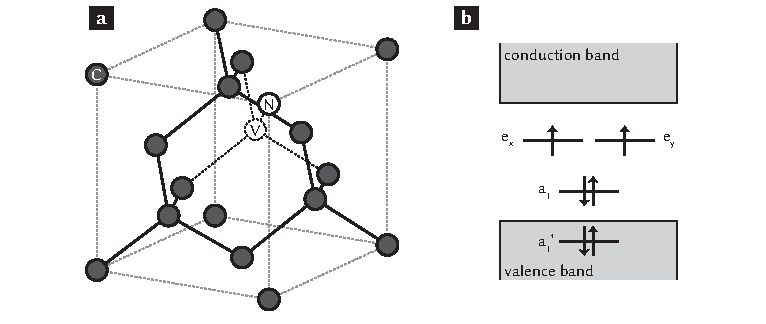
\includegraphics{figure_NV-structure-bernien}
	\caption{\label{fig:tam-fig1-nvstruct} \textbf{Crystal and electronic structure of the NV center} Figure from \cite{Bernien__2014}(a) The Nitrogen-Vacancy center defect is formed by a substitutional nitrogen atom (N) and a missing atom (vacancy, V) at an adjacant position in the diamond lattice (b) The electron occupation of the molecular orbitals in the electronic ground state, following Pauli's exclusion principle. The molecular orbitals are a linear combination of hybridised $sp^3$-orbitals. They are found by using the $C_{3v}$-symmetry of the NV center, taking into account the Coulomb interaction of the diamond nuclei and the lattice electrons with the electrons in the orbitals.}
\end{figure*}

In the electronic ground state, the 6 electrons occupy the molecular orbitals as shown in Fig. \ref{fig:tam-fig1-nvstruct}b. Excluding electron-electron interactions, the electronic ground-, ($^2a^2e$) and excited ($^1a^3e$) state are spin degenerate. This degeneracy is lifted by the Coulomb interaction between the electrons which leads to spin triplet (S = 1) ground-, and excited states ($^3A_2$ and $^3E$ respectively) as well as multiple intermediate spin singlet levels. The $^3A_2$ to $^3E$ transition energy of 1.945 eV lies in the optical regime (637 nm), well within the bandgap of diamond (5.5eV). Since all experimental techniques in this thesis aim to control the NV center in the spin triplet manifold, we will not discuss the singlet levels in further detail. For a more detailed discussion of the electronic structure of the NV-center we refer to a recent review of Doherty \textit{et al} \cite{Doherty_PhysicsReports_2013}.

\begin{figure*}
	\centering
	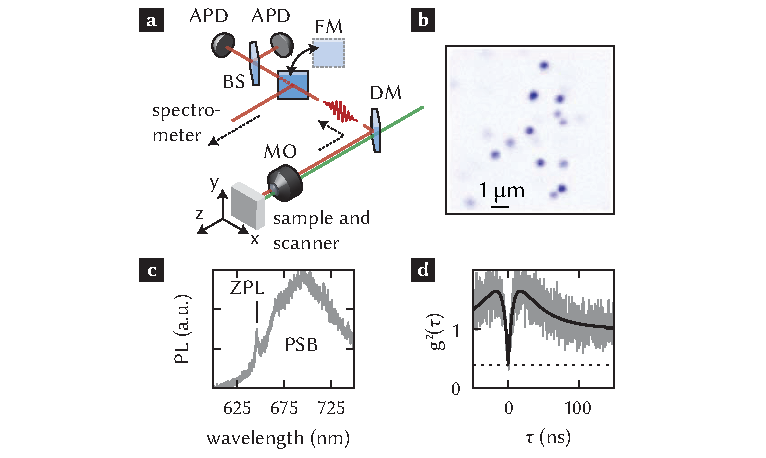
\includegraphics{figure_single_NVs-bernien}
	\caption{\label{fig:tam-fig2-nvstruct} \textbf{Detection of single NV centers} Figure from \cite{Bernien__2014}(a) Confocal microscope setup. The NV centers are excited by focussing a green (532 nm) excitation laser onto the sample using a microscope objective (MO). The sample is mounted on a piezo-stage allowing three-dimensional scans. The emission is spectrally filtered using a dicroic mirror (DM) and via a mechanically switchable mirror (FM) sent either to a spectrometer or to a beamsplitter (BS) followed by two APDs in a HBT-configuration. (b) Confocal scan of a bulk diamond sample. The intensity is plotted as a function of the stage position in \textit{x} and \textit{y}. Blue is higher intensity. (c) Emission spectrum of a single NV center with the zero phonon line at 637 nm and the phonon sideband at higher wavelengths. (d) Second-order autocorrelation function, with $\tau$ the delay between detection events of different detectors. The solid-line is a fit using a three-level model, including dark counts. The slow decay is associated with the decay from the singlet levels.}
\end{figure*}

We identify NV centers in bulk diamond at room-temperature in a home-build confocal microscope setup (Fig. \ref{fig:tam-fig2-nvstruct}a). By scanning the sample and collecting the fluorescence signal with a single photodiode (APD) we find multiple diffraction limited spots, corresponding to NV centers (Fig. \ref{fig:tam-fig2-nvstruct}b). Here we off-resonantly excite the NV center to a phonon level above the $^3E$ level, which quickly decays non-radiatively to $^3E$. The reflections of the excitation are separated from the fluorescence with a dicroic mirror. The emission spectrum from $^3E$ is show in Fig. \ref{fig:tam-fig2-nvstruct}c. It shows a distinct peak around 637 nm, corresponding to the direct decay from $^3E$ to $^3A_2$ (zero phonon line, ZPL) and a broad sideband corresponding to the decay to a phonon level above $^3A_2$ (phonon side band, PSB). To verify that the signal originates from a single emitter, we measure the second-order autocorrelation function $g^2 (\tau)$ in a Hanbury-Brown-Twiss configuration (Fig. \ref{fig:tam-fig2-nvstruct}d). The low probability of simultaneous photon detection ($g^2 (\tau = 0) < 1/2$) confirms that the signal comes from a single emitter.

\section{Single NV center device}

To enhance the collection and excitation efficiency of the NV center, a solid-immersion lens (SIL) is milled in the diamond using a focused ion beam (FIB) \cite{Hadden__2010,Marseglia__2011,Bernien__2014,Jamali__2014} (Fig. \ref{fig:tam-fig3-device}a). For an NV center in the middle of the SIL, the hemisphere ensures that the emission from the NV center reaches the diamond-air surface at normal incidence. This significantly reduces the loss due to total-internal reflection. For precise placement of the SIL, a pre-characterized NV center is located with respect to 1x1 $\mu$m gold markers that are fabricated on the surface of the diamond using electron beam lithography. The hemisphere structure is then created using a gallium ion beam by milling concentric rings of varying diameter around the position of the NV center. After milling the SILs, the sample is cleaned for 30 minutes in a boiling mixture of equal parts of perchloric, sulforic and nitric acid. This step removes the redeposited material during milling. A small conductive layer of gallium atoms that is implanted during the FIB process is removed by reactive-ion etching in an oxygen-plasma. 
\label{sec:devices}
\begin{figure*}
	\centering
	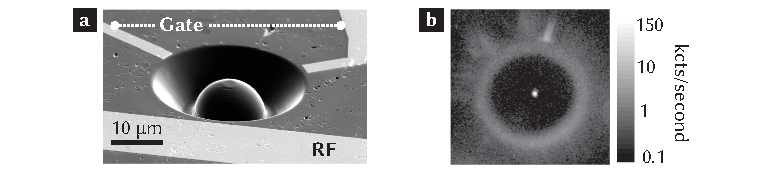
\includegraphics{figure_SIL_finished-bernien}
	\caption{\label{fig:tam-fig3-device} \textbf{} Figure from \cite{Bernien__2014} (a) }
\end{figure*}

A 200 nm thick gold microwave strip line for spin manipulation (Fig \ref{fig:tam-fig7-erabi} and \ref{fig:tam-fig10-nrabi}) and DC gates to DC stark shift the ZPL (see chapter \ref{ch:LDE}) are  fabricated near the SIL using electron beam lithography. Finally a single-layer anti-reflection coating\cite{Yeung__2012} (aluminium oxide) is fabricated on top of the sample to further increase the collection efficiency and reduce the reflection during resonant excitation (see chapter \ref{ch:LDE}).

\section{Addressing the electron excited state}
\label{sec:opticalcontrol}

The spin-orbit and spin-spin interactions introduce a fine splitting to the $^3E$ excited state which can be observed at cryogenic temperatures. The six resulting transitions have a distinct spin character (Fig. \ref{fig:tam-fig4-laserscan}a) and allow for spin-selective optical excitation of the electron. The transitions to the $m_s = 0$ states ($E_x$ and $E_y$) can occur upon absoprtion or emission of a linearly polarized photon, while the four $m_s = \pm 1$ transitions couple to circularly polarized light. The transition frequencies shift when an electric field or strain is applied. For an electric field along the N-V axis this results in an offset to the spectrum, not changing the energy level spacing. A perpendicular electric field affects the difference between the energy levels. As a result, the spectrum of the excited state slightly varies between NV centers due to local differences in strain and electric field. In Fig. \ref{fig:tam-fig4-laserscan}b we show measurements of the spectra of three different NV centres, normalized to have the same parallel strain. The lateral strain is determined from the difference between the transition energies of $E_x$ and $E_y$. The spectra show excellent agreement with the theoretical prediction (dashed lines). The strain typically differs a few tens of GHz between NV centers measured in this thesis.

\begin{figure*}
	\centering
	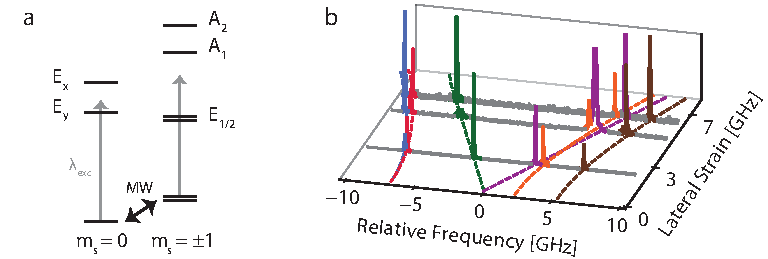
\includegraphics{laserscans}
	\caption{\label{fig:tam-fig4-laserscan} \textbf{Spectrum of the excited state} (a) Energy level diagram of the fine structure of the excited states. There are two levels with spin $m_s = 0$ ($E_x$,$E_y$) and four $m_s = \pm 1$ levels ($A_1$,$A_2$,$E_1$ and $E_2$). At finite strain the degeneracies between $E_x$,$E_y$ and $E_1$,$E_2$ are lifted. (b) The energy spectrum for three different NV centers is measured by varying the frequency of the excitation laser and detecting the fluorescence in the PSB. The observed transitions $E_1$ (blue), $E_2$ (red), $E_y$ (green), $E_x$ (purple), $A_1$ (orange) and $A_2$ (brown) are color coded and agree well with the theoretical prediction (colored dashed lines). For each scan the transition energies $\Delta E_x$ and $\Delta E_y$ are determined to calculate the lateral ($\frac{\Delta E_x-\Delta E_y}{2}$) and parallel ($\frac{\Delta E_y+\Delta E_x}{2}$) strain. The parallel strain is then substracted for each scan. Laser frequency is with respect to 470.4 THz.}
\end{figure*}

To address the spin-selective optical transitions in an experiment, we first verify that the NV center is in the $NV^-$ state and that the lasers are resonant with the desired transitions before each experimental run. During this charge-resonance (CR) check, we simultaneously apply two red lasers and monitor the fluorescence (Fig. \ref{fig:tam-fig4-cr}a). The lasers can only excite the electron spin for the NV center in $NV^-$ and the number of detected photons is highest when one red lasers is resonant with a $m_s = 0$ transition and the other with a $m_s=\pm1$ transition. We therefore compare the signal to a threshold and only continue with the experimental sequence when the threshold is passed (Fig. \ref{fig:tam-fig4-cr}b). When the number of detected photons is below the threshold we apply a green (523 nm) laser, perform another CR check and repeat until success. The green laser can repump the center to $NV^-$ by exciting trapped charges in the environment, but also induces spectral diffusion of the optical transitions since the local electric field is affected by the charge configuration in the environment. As an alternative to the green laser, a yellow laser ($\lambda \approx 575$ nm) can be used to resonantly excite the $NV^0$ zero phonon line \cite{Siyushev_Phys.Rev.Lett._2013}. 

\begin{figure*}
	\centering
	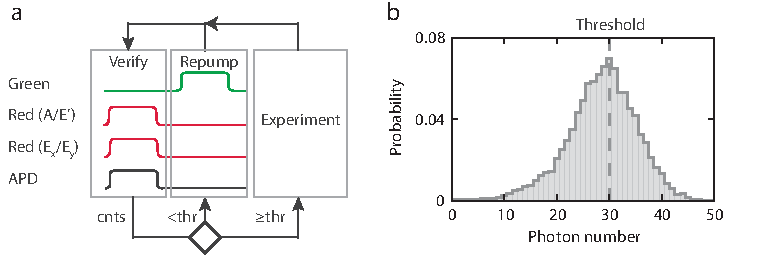
\includegraphics{CR}
	\caption{\label{fig:tam-fig4-cr} \textbf{Verifying the charge state and laser resonances} (a) Schematic of the experimental sequence to verify the charge state of the NV center and the laser resonances. The process is controlled by an ADwin microprocessor which turns on the two red lasers and compares the number of photons detected by the avalanche photodiode (APD) to a predetermined threshold (verify stage). When the number of detected photons is below the threshold a green laser is applied to prepare the $NV^-$ state (repump stage), otherwise the experimental sequence is initiated. (b) Photon number distribution during the verification stage, conditioned on the previous CR check being successful. }
\end{figure*}

The electron spin is initialized by selectively exciting a single transition\cite{Robledo_Nature_2011}: $E_x$ or $E_y$ to prepare $m_s = \pm 1$ or $A_1$/$A_2$/$E'$ to prepare $m_s=0$. The slight spin mixing of the excited states provides an optical pumping mechanism to prepare the opposite spin state (\ref{fig:tam-fig5-SP})a). The fluorescence observed during initialization (\ref{fig:tam-fig5-SP})b) exponentially decreases with the probability that the spin has flipped to a dark state that can not be excited by the pumping laser. The signal is fitted to an exponential decay to extract a lower bound for the preparation fidelity. To ensure that a pure state is prepared (as opposed to a mixture of $m_s = \pm 1$) the electron spin is typically initialized in $m_s = 0$, for this state we find a lower bound of $(99.7 \pm 0.1) \%$.

\begin{figure*}
	\centering
	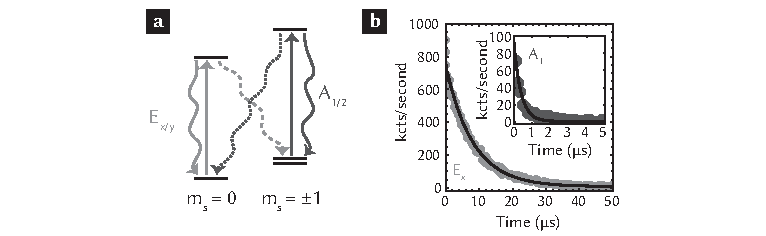
\includegraphics{figure_spinpumping-bernien}
	\caption{\label{fig:tam-fig5-SP} Figure from \cite{Bernien__2014} \textbf{Initialization by spin pumping} (a) Energy levels used to initialize (and readout) the electron spin. We excite transitions with a well-defined spin character of either $m_s = 0$ (bright arrows) or $m_s= \pm 1$ (dark arrows), resulting in spin-conserving optical cycling (indicated by bended solid arrows). Dashed arrows indicate the spin non-conserving decay paths. (b) Observed fluorescence when exciting $E_x$ ($A_1$) with the spin initially prepared in $m_s = \pm 1$ ($m_s = 0$). The signal is fitted to a single exponential with an offset to account for dark counts. From the fit we find a lower limit for the initialization fidelities: $(99.7 \pm 0.1) \%$ for $m_s = 0$ and $(99.2 \pm 0.1) \%$ for $m_s=\pm 1$.}
\end{figure*}

The observed fluorescence upon selective excitation provides a means to detect the electron spin state in a single shot\cite{Robledo_Nature_2011}. To characterize the readout we plot the distribution of photons detected in the PSB collected during a 10 $\mu s$ laser pulse exciting $E_x$ (fig \ref{fig:tam-fig6-ssro}a). The distributions are clearly separated depending on the initial spin state, allowing us to assign $m_s = 0$ to the cases where one or more photons are detected and $m_s = \pm 1$ otherwise. The combined readout and initialization fidelity for $m_s = \pm 1$ ($F_1 = .989 \pm .001$) is reduced by detector dark counts and off-resonant excitation, while for $m_s = 0$ ($F_1 = .956 \pm .003$) the error is governed by the instances where the spin is flipped before a photon is detected. This can be seen in fig \ref{fig:tam-fig6-ssro}b where the readout fidelities are plotted as a function of readout duration. The fidelity for $m_s = 0$ initially increases with readout time and then saturates indicating that the spin has flipped with high probability. The optimal mean readout fidelity ($F_{ro} = \frac{F_0+F_1}{2} = 0.973 \pm 0.002$) is reached after $10 \mu s$.

\begin{figure*}
	\centering
	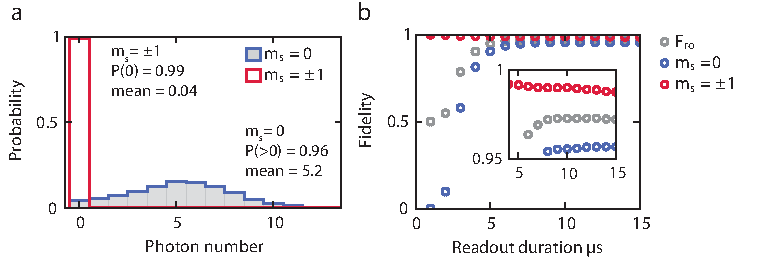
\includegraphics{ssro}
	\caption{\label{fig:tam-fig6-ssro} \textbf{Single shot readout} (a) Histograms of the number of detected photons in the PSB for initial state $m_s = 0$ (blue) and $m_s=\pm 1$ (red) during a 10 $\mu s$ readout on $E_x$. (b) Fidelities for reading out the electron spin state initially prepared in $m_s = 0$ (blue) and $m_s = \pm 1$ (red) as a function of readout duration. The mean readout fidelity is plotted in grey. The inset is a zoom of the region where the optimal mean readout fidelity is reached.}
\end{figure*}

\section{Ground state spin control and coherence}

In the orbital ground state, the $m_s = 0$ and $m_s = \pm 1$ states are separated by the zero-field splitting $D \approx 2.88$ GHz, while an external magnetic field lifts the degeneracy between $m_s = +1$ and $-1$ via the zeeman splitting. The hamiltonian is given by

\begin{equation}
H_{GS} = D^2 S_z + \gamma_e \mathbf{B} \cdot \mathbf{S}
\end{equation}

with $\mathbf{S} =[S_x,S_y,S_z]$,  $S_i$ the pauli spin matrices for a spin-1 particle and $\gamma_e = 2.8$ MHz/G the gyromagnetic ratio of the electron. We define our qubit in the $m_s = 0 :\ket{0}$ and $m_s = -1 : \ket{1}$ states (alternatively the $m_s = + 1$ state can be used to encode $\ket{1}$). The electron spin is manipulated with electron spin resonance techniques by sending an ac current through the stripline generating an oscillating magnetic field at the location of the NV center. At the resonance condition the frequency of the control field matches the energy difference between the $\ket{0}$ and $\ket{1}$ states resulting in coherent Rabi oscillations between those levels as shown in fig \ref{fig:tam-fig7-erabi}. Arbitrary qubit rotations are implemented by calibrating the amplitude (which sets the rabi frequency) and length of the control pulses.


Spin manipulation with ESR techniques. (Fig. \ref{fig:tam-fig7-erabi})

Figure to add: Coherence times $T_2^{*}$, $T_2$ and dynamical decoupling.

\label{sec:groundstatecontrol}
\begin{figure*}
	\centering
	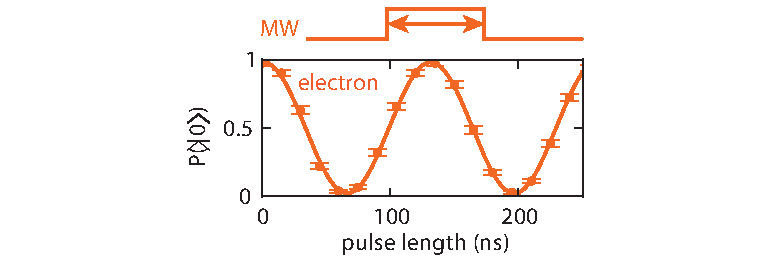
\includegraphics{electron_rabi}
	\caption{\label{fig:tam-fig7-erabi} \textbf{} (a) Coherent qubit rotations of the electron spin are performed by varying the length of a MW pulse. The signal is corrected to account for imperfect readout and initialization. Solid line is a sinusoidal fit from which we determine the Rabi frequency $(7.67 \pm 0.02)$ MHz}
\end{figure*}

%\begin{figure*}
%	\centering
%	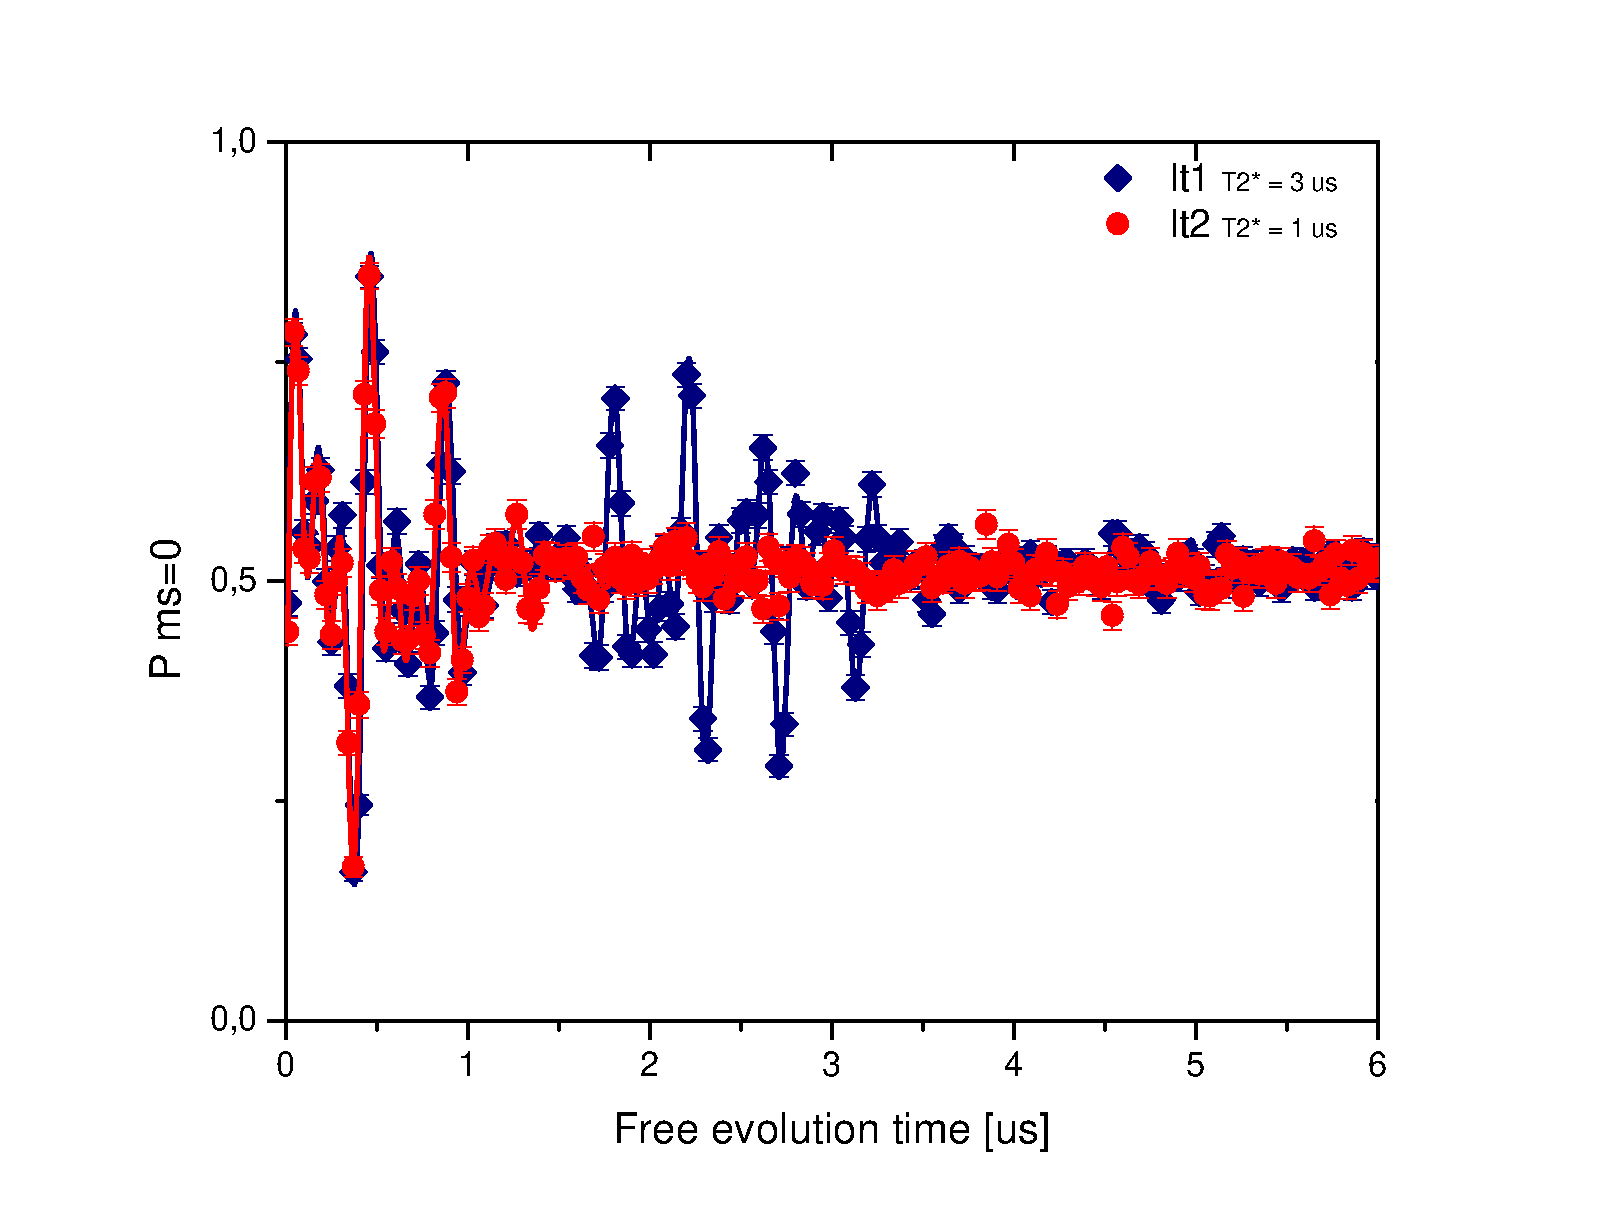
\includegraphics{ramsey-LDE}
%	\caption{\label{fig:tam-fig8-eramsey} \textbf{} (a) }
%\end{figure*}

\begin{figure*}
	\centering
	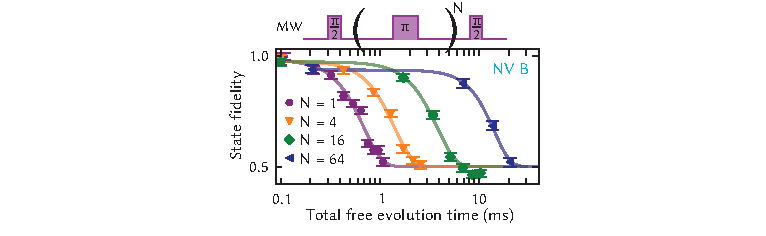
\includegraphics{DD-LDE_bernien}
	\caption{\label{fig:tam-fig9-DD} \textbf{Dynamical Decoupling of the electron spin} (a) }
\end{figure*}

\section{Coupling to nuclear spins}

Hyperfine coupling to nitrogen spin and NMR.

Figure to add: ESR with visible splitting of the $^{14}N$ spin and nuclear rabi
%\label{sec:nuclearspins}
%\begin{figure*}
%	\centering
%	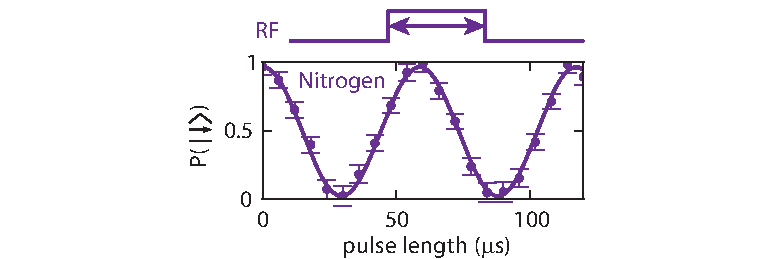
\includegraphics{nitrogen_rabi}
%	\caption{\label{fig:tam-fig10-nrabi} \textbf{} (a) }
%\end{figure*}
%\section{Quantum measurements}


%\section{Methods}



\newpage
\bibliographystyle{../thesis}
\bibliography{tam}




\graphicspath{{./ch_adptv_msmnt_cntrl/figures/}}


\chapter[Manipulating a qubit through the backaction of adaptive measurements]{Manipulating a qubit through the backaction of sequential partial measurements \\ and real-time feedback }
\label{ch:AMC}

\begin{center} 
    \vspace{-1cm} {M.S.~Blok$^*$, C.~Bonato$^*$, M.L.~Markham, D.J. ~Twitchen, V.V. ~Dobrovitski and R.~Hanson} 
\end{center}


{\renewcommand{\thefootnote}{}\footnote{This chapter has been published in
    {\em Nature Physics} \textbf{10}, 189-193 (2014).}\footnote{$^*$ these authors contributed equally to this work}}


\vspace{-0.5cm} 
Quantum measurements not only extract information from a system but also alter its state. Although the outcome of the measurement is probabilistic, the backaction imparted on the measured system is accurately described by quantum theory ~\cite{Guerlin_Nature_2007,Hatridge_Science_2013,Murch_Nature_2013}. Therefore, quantum measurements can be exploited for manipulating quantum systems without the need for control fields~\cite{Ashhab_PhysRevA_2010,Wiseman_NatureNV_2011}. We demonstrate measurement-only state manipulation on a nuclear spin qubit in diamond by adaptive partial measurements. We implement the partial measurement via tunable correlation with an electron ancilla qubit and subsequent ancilla readout~\cite{Brun_PhysRevA_2008,Groen_PRL_2013}. We vary the measurement strength to observe controlled wavefunction collapse and find post-selected quantum weak values~\cite{Brun_PhysRevA_2008,Groen_PRL_2013,Aharonov_PRL_1988,Pryde_PRL_2005,Dressel_ArXiv_2013}. By combining a novel quantum non-demolition readout on the ancilla with real-time adaption of the measurement strength we realize steering of the nuclear spin to a target state by measurements alone. Besides being of fundamental interest, adaptive measurements can improve metrology applications~\cite{Cappellaro_PhysRevA_2012,Higgins_Nature_2007} and are key to measurement-based quantum computing~\cite{Raussendorf_PRL_2001,Prevedel_Nature_2007}.


\clearpage

\section{Introduction}
Measurements play a unique role in quantum mechanics and in quantum information processing. The backaction of a measurement can be used for state initialization~\cite{Robledo_Nature_2011,Riste_PRL_2012}, generation of entanglement between non-interacting systems~\cite{Chou_Nature_2005,Moehring_Nature_2007,Pfaff_NatPhys_2012,Riste_Nature_2013}, and for qubit error detection~\cite{Chiaverini_Nature_2004}. These measurement-based applications require either post-selection or real-time feedback, as the outcome of a measurement is inherently probabilistic. Recent experiments achieved quantum feedback control on a single quantum system~\cite{Riste_Nature_2013, Gillett_PRL_2010,Sayrin_Nature_2011,Vijay_Nature_2012} by performing coherent control operations conditioned on a measurement outcome.

Here, we realize real-time adaptive measurements and exploit these in a proof-of-principle demonstration of measurement-only quantum feedback. Our protocol makes use of partial measurements that balance the information gain and the measurement backaction by varying the measurement strength. We accurately control the measurement strength and the corresponding backaction in a two-qubit system by tuning the amount of (quantum) correlation between the system qubit and an ancilla qubit, followed by projective readout of the ancilla~\cite{Brun_PhysRevA_2008,Groen_PRL_2013}. In general, the backaction of sequential partial measurements leads to a random walk~\cite{Guerlin_Nature_2007,Hatridge_Science_2013,Murch_Nature_2013} but by incorporating feedback, multiple measurements can direct the trajectory of a qubit towards a desired state~\cite{Ashhab_PhysRevA_2010,Wiseman_NatureNV_2011}. Real-time adaptive measurements are a key ingredient for quantum protocols such as one-way quantum computing~\cite{Raussendorf_PRL_2001,Prevedel_Nature_2007} and Heisenberg-limited phase estimation~\cite{Cappellaro_PhysRevA_2012,Higgins_Nature_2007}.

We implement the adaptive partial measurements in a nitrogen vacancy (NV) center in synthetic diamond. We define the system qubit by the nuclear spin of the NV host nitrogen ($\ket{\downarrow}$: $m_I$=0, $\ket{\uparrow}$: $m_I$= -1), and the ancilla qubit by the NV electron spin ($\ket{0}$: $m_S$=0, $\ket{1}$: $m_S$=-1) (Fig.\,\ref{fig:amc-fig1}a). The ancilla is initialized and read out in a single shot with high fidelity using spin-selective optical transitions~\cite{Robledo_Nature_2011}. We perform single-qubit operations on the ancilla by applying microwave frequency pulses to an on-chip stripline.


\section{Variable-strength measurement}
\begin{figure*}
	\centering
	\includegraphics{fig1_twocolumns}
	\caption{\label{fig:amc-fig1} \textbf{Partial measurement of a spin qubit in diamond.} (a) The NV center is a natural two-qubit system where the system qubit is defined by the $^{14}N$ nuclear spin and the ancilla qubit is defined by the electron spin. A solid-immersion-lens is deterministically fabricated on top of the selected NV center to increase the photon collection efficiency. Control fields for single qubit rotations are generated by applying a current to the gold stripline (yellow).  (b) A tunable strength measurement is implemented by a Ramsey-type gate on the ancilla. We plot the probability to measure the state $\ket{0}$  for the ancilla, as a function of interaction time $\tau$, for two system input states $\ket{\downarrow}$ (red) and $\ket{\uparrow}$ (blue). The Bloch-spheres show the state of the system (purple) and ancilla (orange) after the entangling-gate for the different input states (red and blue vectors). The colour bar represents the measurement strength, proportional to $\sin{\theta}$, where $\theta=\frac{A \tau}{2}$. Blue corresponds to a projective measurement and white to no measurement. Solid lines are a  fit to the function $y_0 + e^{-( \frac{\tau}{T_2^*})^2} \cos{(A \tau + \delta)} $. From the phase offset $\delta$ we find the weakest measurement we can perform, corresponding to $\theta = 5^{\circ}$. This is limited by free evolution of the ancilla during the pulses.(see Methods). Error bars depict 68 $\%$ confidence intervals. Sample size is 500 for each data point. }
\end{figure*}

We realize the variable-strength measurement by correlating the system qubit with the ancilla through a controlled-phase-type gate (Fig.\,\ref{fig:amc-fig1}b) that exploits the hyperfine interaction, which (neglecting small off-diagonal terms) has the form $\hat{H}_{hf}=A\hat{S}_{z}\hat{I}_{z}$ (with $A = 2 \pi \times 2.184 \pm 0.002$ MHz and $\hat{S}_{z}, \hat{I}_{z}$ the three-level Pauli z-operators for the electron, nuclear spin respectively).  During free evolution, the ancilla qubit precession is conditional on the state of the system qubit. We choose the rotating frame such that the ancilla rotates clockwise (anti-clockwise) around the z-axis if the system qubit is in $\ket{\uparrow}$ ($\ket{\downarrow}$) and vary the interaction time $\tau$. For $\tau = 0$, there is no correlation between the ancilla and the system, whereas for $\tau = \frac{\pi}{A}$, corresponding to the rotation angle $\theta = 90^{\circ}$, the two are maximally correlated. A subsequent rotation and projective readout of the ancilla then implements a measurement of the system qubit, with a measurement strength that can be accurately tuned by controlling the interaction time $\tau$. A mathematical derivation  can be found in the methods.

We investigate the measurement-induced backaction by preparing an initial state of the system ($\ket{\up},\ket{x}$ and $\ket{y}$) and performing a partial measurement with strength $\theta$, followed by state tomography (Fig.\,\ref{fig:amc-fig2}a). First, we neglect the outcome of the partial measurement, which is mathematically equivalent to taking the trace over the state of the ancilla qubit. In this case the backaction is equivalent to pure dephasing as can be seen by a measured reduction of the length of the Bloch vector (Fig.\,\ref{fig:amc-fig2}b). Next, we condition the tomography on the ancilla measurement yielding state $\ket{0}$ (Fig.\,\ref{fig:amc-fig2}c). We observe that for a weak measurement $(\theta = 5^{\circ})$, the system is almost unaffected, whereas for increasing measurement strength it receives a stronger kick towards $\ket{\uparrow} $(Fig.\,\ref{fig:amc-fig2}c). Crucially, we find that the length of the Bloch vector is preserved in this process, as expected for an initially pure state. This shows that the partial collapse is equivalent to a qubit rotation that is conditional on the measurement strength and outcome and on the initial state. By performing quantum process tomography, we find that both measurement processes agree well with the theoretical prediction (the process fidelities are 0.986 $\pm$ 0.004 and 0.94 $\pm$ 0.01 for the unconditional and conditional process, respectively; see Methods).


\begin{figure}
	\centering
	\includegraphics{fig2_partial_measurement_backaction}
	\caption{\label{fig:amc-fig2} \textbf{Measurement backaction for variable-strength measurement}. (a) We prepare an initial state  of the system ($\ket{\uparrow}$,  $\ket{x}$ and  $\ket{y}$), perform a partial measurement with strength $\theta$, and characterize the measurement backaction on the system by quantum state tomography. Quantum state tomography is implemented by an ancilla-assisted projective measurement, performed with the same protocol, setting $\tau = 229$ ns for $\theta = 90^{\circ}$. The nuclear spin basis rotation is performed with a $\frac{\pi}{2}$ radio-frequency pulse (along either $x$ or $y$). The basis rotation pulse for the tomography is applied before the readout of the ancilla, to avoid the dephasing induced by the state-characterization measurement (see main text). The data is corrected for errors in the readout and initialization of the system qubit, both of which are obtained from independent measurements (see methods). (b,c)  Measurement backaction for a partial measurement of increasing strength, independent of the measurement result for the ancilla qubit (b), or conditioned on the ancilla in  $\ket{0}$ (c). }
\end{figure}

\section{Generalized weak value}
By combining a partial measurement with post-selection on the outcome of a subsequent projective measurement, we can measure the generalized weak value $_{f} \langle I_{z} \rangle$ (conditioned average of contextual values \cite{Dressel_PRL_2010}, see methods) of the nuclear spin in the $z$-basis. In the limit of zero measurement strength ($\theta = 0^{\circ}$), this quantity approximates the weak value \cite{Aharonov_PRL_1988} $W = \frac{\bra{\psi_f} \hat{I}_z \ket{\psi_i}}{\bra{\psi_f} \psi_i \rangle}$ , where $ \psi_i (\psi_f )$ is the initial (final) state of the nucleus and from here we define $\hat{I}_z$ as the Pauli $z$-operator reduced to a two-level system with eigenvalues +1 and $-$1. By post-selecting only on the final states having small overlap with the initial state, $_{f} \langle I_{z} \rangle$ can be greatly amplified to values that lie outside the range of eigenvalues of the measured observable. As shown in Fig.\,\ref{fig:amc-fig3}, by sweeping the angle between the initial and final states we observe up to tenfold amplification ($_{f} \langle I_{z} \rangle = 10 \pm 3$) compared to the maximum eigenvalue of $I_{z}$ ($+1$). This amplification is the highest reported for a solid-state system to date\cite{Groen_PRL_2013}. As predicted \cite{Williams_PRL_2008}, we observe that values of  $_{f} \langle I_{z} \rangle$ lying outside of the range of eigenvalues of $I_{z}$ can be found for any finite measurement strength.

\begin{figure}
	\centering
	\includegraphics{fig3_weak_value}
	\caption{\label{fig:amc-fig3} \textbf{Generalized quantum weak value}. Measurement of a generalized weak value for the nuclear-spin qubit, performed by a partial measurement of strength $\theta$, followed by a strong measurement and post-selection of the state  $\ket{\downarrow}$, as a function of the basis rotation angle $\phi$ of the strong measurement (Fig.\,\ref{fig:amc-fig2}a). Solid lines are simulations using independently determined parameters. The asymmetry in the curve can be explained by asymmetric nuclear spin flips arising during ancilla initialisation by optical excitation of the forbidden transition of $E_{y}$ (see methods). Inset: the generalized weak values as a function of the strength $\theta$ of the partial measurement, setting the basis rotation angle of the strong measurement to the optimal value  $\phi = \frac{\pi}{2} - \theta$. All error bars depict 68 $\%$ confidence intervals. The sample size varies per data point because each data point has different post-selection criterion.}
\end{figure}

\section{QND-measurement of the ancilla qubit}
Using the partial measurements for measurement-based feedback requires reading out the ancilla without perturbing the system qubit. In our experiment the system qubit can dephase during ancilla readout both through a spin-flip of the electron in the course of optical excitation (Fig.\,\ref{fig:amc-fig4}b) and as a result of the difference in the effective nuclear g-factor in the electronic ground- and optically excited state~\cite{Jiang_PRL_2008}. Note that for the characterization of a single partial measurement (Fig.\,\ref{fig:amc-fig2}) we circumvent this dephasing by interchanging the measurement basis rotation and the ancilla readout; this interchange is not possible for real-time adaptive measurements.

\begin{figure*}
	\centering
	\includegraphics{fig4_qnd_electron}
	\caption{\label{fig:amc-fig4} \textbf{Quantum non-demolition measurement of the ancilla qubit} (a) The ancilla is initialized in $\ket{0}$ ($\ket{1}$) by optically pumping the $A_2$ ($E_y$) transition. The ancilla is then read out by exciting the $E_y$ transition for 100 $\mu$s (conventional readout), or until a photon was detected (dynamical-stop readout). Finally, we verify the post-measurement state with a conventional readout. (b) Fidelity of the post-measurement state of the ancilla for conventional readout (left graph) and dynamical-stop readout (right graph). Results are corrected for the infidelity in the final readout.  All error bars depict 68 $\%$ confidence intervals. Sample size per datapoint is 5000 }
\end{figure*}

To mitigate the nuclear dephasing during ancilla readout we reduce the ancilla spin-flip probability using a dynamical-stop readout technique. We partition the optical excitation time in short ($1~ \mu$s) intervals and we stop the excitation laser as soon as a photon is detected, or after a predetermined maximum readout time when no photon is detected (Fig.\,\ref{fig:amc-fig4}a). This reduces redundant excitations without compromising the readout fidelity. In Fig.\,\ref{fig:amc-fig4}b we show the correspondence between pre- and post-measurement states for the two eigenstates of the ancilla. For the state $\ket{0}$ the dynamical-stop readout increases the fidelity ($F = \bra{\psi_i}\rho_m \ket{\psi_i}$, where $\rho_m$ is the density matrix of the system after the ancilla readout) from 0.18 $\pm$ 0.02 to 0.86 $\pm$ 0.02. The latter fidelity is solely limited by the cases where the spin flipped before a photon was detected: we find $F = 1.00 \pm 0.02$ for the cases in which a photon was detected. As expected, the fidelity is high ($F = 0.996 \pm 0.006$) for input state $\ket{1}$ as this state is unaffected by the excitation laser. The dynamical-stop technique thus implements a quantum non-demolition (QND) measurement of the ancilla electron spin with an average fidelity of 0.93 $\pm$ 0.01 for the post-measurement state.

The dynamical-stop readout of the ancilla significantly reduces the dephasing of the nuclear spin qubit during measurement as shown in Fig.\,\ref{fig:amc-fig5}. Starting with the nuclear spin in state $\ket{x} = \frac{\ket{0} + \ket{1}}{\sqrt{2}}$, a conventional readout of the ancilla completely dephases the nuclear spin, leading to a state fidelity with respect to $\ket{x}$ of 0.5. In contrast, the fidelity of the dynamical-stop readout saturates to 0.615 $\pm$ 0.002 (probably limited by changes in the effective g-factor of the nuclear spin). The dynamical-stop readout thus leaves the system in a coherent post-measurement state that can be used in a real-time feedback protocol. 

\begin{figure*}
	\centering
	\includegraphics{fig5_qnd_nuclear_spin}
	\caption{\label{fig:amc-fig5} \textbf{System qubit coherence during ancilla readout}. Coherence of the system qubit state after ancilla readout. For the dynamical-stop protocol we define the ancilla readout time as the predetermined maximum readout time. The graph shows the fidelity of the system with respect to $\ket{x}$ for conventional readout (red) and dynamical-stop readout (blue). The $z$-component of the system is unaffected as shown by the constant fidelity with respect to $\ket{\uparrow}$ (grey). All error bars depict 68 $\%$ confidence intervals. Sample size per datapoint is 2000 }
\end{figure*}

\section{Control by adaptive measurements}
Preserving coherence of the post-measurement state enables a proof-of-principle realization of measurement-only control, by implementing sequential measurements and tuning the strength of the second measurement in real time conditioned on the outcome of the first measurement (Fig.\,\ref{fig:amc-fig6}a). We choose as our target the creation of the state $\ket{\psi} = \cos{(\frac{\pi}{4}+\frac{\theta_1}{2})}\ket{\downarrow}+\cos{(\frac{\pi}{4}-\frac{\theta_1}{2})}\ket{\uparrow}$ from initial state $\ket{x}$ using only partial measurements of $\hat{I}_z$. The first measurement with strength $\theta_1$ will prepare either the desired state, or the state $\ket{\psi_{wrong}} =  \cos{(\frac{\pi}{4}-\frac{\theta_1}{2})}\ket{\downarrow}+\cos{(\frac{\pi}{4}+\frac{\theta_1}{2})}\ket{\uparrow}$ , each with probability 0.5. We adapt the strength of the second measurement $\theta_2$ according to the outcome of the first measurement: we set $\theta_2 = 0$ if the first measurement directly yielded the target state, but if the wrong outcome was obtained we set the measurement strength to

\begin{equation}
\theta_2 = \sin{^{-1}\left[2 \frac{\sin{\theta_1}}{1 + \sin{^2 \theta_1}}\right]},
\end{equation}

such that the second measurement will probabilistically rotate the qubit to the target state (see methods). The total success probability of this two-step protocol is  $p_{suc} = \frac{1}{2}(1 + \cos{\theta_1})$ and a successful event is heralded by the outcome of the ancilla readout. In principle the protocol can be made fully deterministic~\cite{Ashhab_PhysRevA_2010} by incorporating a reset in the form of a projective measurement along the $x$-axis.

To find the improvement achieved by the feedback, we first compare the success probability of our adaptive measurement protocol to the success probability for a single measurement (Fig.\,\ref{fig:amc-fig6}b right panel). The success probability clearly increases with the adaptive protocol and is proportional to the readout fidelity of the $\ket{0}$ state of the ancilla, which is maximum for readout times  \textgreater~25~$\mu$s. The fidelity of the final state (Fig.\,\ref{fig:amc-fig6}b left panel) is limited by the remaining dephasing of the system during readout of the ancilla as shown in Fig.\,\ref{fig:amc-fig5}. This constitutes the trade-off between success probability and state fidelity. 

We show that the increase in success probability is enabled by feedback by comparing the final state fidelity with and without feedback (Fig.\,\ref{fig:amc-fig6}b left panel). In principle the success probability can be increased in the absence of feedback by accepting a certain number of false measurement outcomes at the cost of a reduced fidelity. We calculate the maximum fidelity that can be achieved in this way by performing only the first measurement and increasing the success probability to that of the adaptive protocol using post-selection (grey line in Fig.\,\ref{fig:amc-fig6}b, left panel). We find that the measured state fidelity in the adaptive protocol is above this bound (Fig.\,\ref{fig:amc-fig6}b, green area), which indicates that the adaptive measurement indeed successfully corrects the kickback from the first measurement, thus yielding a clear advantage over open-loop protocols.



We note that, in contrast to pioneering adaptive measurement experiments on photons that only used experimental runs in which a photon was detected at each measurement stage~\cite{Prevedel_Nature_2007}, our protocol is fully deterministic in the sense that the partial measurement always yields an answer. In particular, the data in Fig.\,\ref{fig:amc-fig6} includes all experimental runs and thus no post-selection is performed, as desired for future applications in metrology and quantum computing. 

The performance of the protocol can be further improved by increasing the ancilla readout fidelity (either by improving the collection efficiency or reducing spin-flip probability) and by further reducing the dephasing of the system during readout. A particularly promising route is to use nuclear spins farther away from the NV center (for example carbon-13 spins) that have much smaller hyperfine couplings~\cite{Zhao_NatureNano_2012,Taminiau_PRL_2012,Kolkowitz_PRL_2012} and are more robust against changes in the orbital state of the electron spin.

\begin{figure*}
	\centering
	\includegraphics{fig6_adaptive_protocol}
	\caption{\label{fig:amc-fig6} \textbf{Manipulation of a nuclear spin state by sequential partial adaptive measurements with real-time feedback.} (a) Adaptive measurement protocol. The ancilla qubit is initialized in $\ket{0}$ and the system qubit is prepared in $\ket{x}$. The strength of the second measurement ($\theta_2$) is adjusted according to the outcome of the first measurement. The system is analysed by state tomography at each intermediate step. The result of the tomography is plotted on the bloch spheres (blue vector) and compared with the ideal case (grey vector). (b) Fidelity of the output state with respect to the target state as a function of ancilla readout time (dynamical-stop readout) with feedback (only the cases where the protocol heralds success). The grey line is obtained by performing one measurement and adding negative results to artificially increase the success probability to that of the adaptive protocol (red line in right panel). In the right panel we show the probability that the protocol heralds success for one measurement and for the adaptive protocol.  }
\end{figure*}

Our work is the first experimental exploration of a fundamental concept of control-free control \cite{Jordan_PRB_2006, Ashhab_PhysRevA_2010, Wiseman_NatureNV_2011} . Furthermore, the use of adaptive measurements as presented here can increase the performance of spin-based magnetometers \cite{Cappellaro_PhysRevA_2012, Higgins_Nature_2007}. Finally, our results can be combined with recently demonstrated methods for generating entanglement between separate nitrogen vacancy centre spins \cite{Bernien_Nature_2013, Dolde_NatPhys_2013}. Taken together, these techniques form the core capability required for one-way quantum computing, where quantum algorithms are executed by sequential adaptive measurements on a large entangled 'cluster' state \cite{Raussendorf_PRL_2001, Prevedel_Nature_2007}.

%In conclusion, we implemented sequential partial measurements and showed that by adjusting the measurement strength in real-time we can steer a quantum system towards a desired state. Our work is the first experimental exploration of a fundamental concept in the field of quantum measurement and control~\cite{Wiseman_NatureNV_2011} that may find application in systems where control fields are difficult to generate. Furthermore, the use of adaptive measurements as presented here can increase the performance of spin-based magnetometers~\cite{Cappellaro_PhysRevA_2012,Higgins_Nature_2007}. Finally, our results can be combined with recently demonstrated methods for generating entanglement between separate NV center spins~\cite{Bernien_Nature_2013,Dolde_NatPhys_2013}. Taken together, these techniques form the core capability required for one-way quantum computing, where quantum algorithms are executed by sequential adaptive measurements on a large entangled ‘cluster’ state~\cite{Raussendorf_PRL_2001,Prevedel_Nature_2007}.
\section{Methods}
We use a naturally-occurring nitrogen-vacancy center in high-purity type IIa CVD diamond, with a \textless 111\textgreater-crystal orientation obtained by cleaving and polishing a \textless100\textgreater -substrate. Experiments are performed in a bath cryostat, at the temperature of 4.2 K, with an applied magnetic field of 17 G. Working at low-temperature, we can perform efficient electron spin initialization (F = 0.983 $\pm$ 0.006) and single-shot readout (the fidelity is 0.853 $\pm$ 0.005 for $m_S = 0$ and 0.986 $\pm$ 0.002 for $m_S = -1$) by spin-resolved optical excitation~\cite{Robledo_Nature_2011}. Initialization of the nuclear spin is done by measurement~\cite{Robledo_Nature_2011}, with fidelity  0.95~$\pm$~0.02. Single-qubit operations can be performed with high accuracy using microwave (for the electron) and radio-frequency (for the nucleus) pulses applied to the gold stripline. Note that the single-qubit operations on the nucleus are only used for state preparation and tomography, but not in the feedback protocol. The dephasing time $T_2^*$ is (7.8~$\pm$~0.2)~ms for the nuclear spin and (1.35~$\pm$~0.03)~$\mu$s for the electron spin. 
\newpage
\bibliographystyle{../thesis}
\bibliography{amc}





\graphicspath{{./ch_adptv_msmnt_magnetometry/figures/}}


\chapter[Optimized quantum sensing using real-time adaptive measurements]{ Optimized quantum sensing with a single electron spin using real-time adaptive measurements}
\label{ch:AMM}

\begin{center} 
    \vspace{-1cm} {C.~Bonato$^*$, M.S.~Blok$^*$, H.T. ~Dinani, D.W. ~Berry, M.L. ~Markham, D.J. ~Twitchen  and R.~Hanson} 
\end{center}

{\renewcommand{\thefootnote}{}\footnote{This chapter has been submitted to
    {\em Nature Nanotechnology} (2015).}\footnote{$^*$ these authors contributed equally to this work}}

\vspace{-0.5cm} 
Quantum sensors based on single solid-state spins promise a unique combination of sensitivity and spatial resolution ~\cite{Giovannetti_NatPhoton_2011,Higgins_Nature_2007,Degen_APL_2008,Taylor_NatPhys_2008,Maze_Nature_2008,Balasubramanian_Nature_2008,Balasubramanian_NatMater_2009,Dolde_NatPhys_2011,Acosta_Phys.Rev.Lett._2010,Toyli_PNAS_2013,Ovartchaiyapong_NatCommun_2014,LeSage_Nature_2013,Kaufmann_PNAS_2013,Kucsko_Nature_2013,Shi_Science_2015,Maletinsky_NatNano_2012,Staudacher_Science_2013,Mamin_Science_2013,Tetienne_Science_2014,Kolkowitz_Science_2015}. The key challenge in sensing is to achieve minimum estimation uncertainty within a given time and with a high dynamic range. Adaptive strategies have been proposed to achieve optimal performance but their implementation in solid-state systems has been hindered by the demanding experimental requirements. Here we realize adaptive d.c. sensing by combining single-shot readout of an electron spin in diamond with fast feedback. By adapting the spin readout basis in real time based on previous outcomes we demonstrate a sensitivity in Ramsey interferometry surpassing the standard measurement limit. Furthermore, we find by simulations and experiments that adaptive protocols offer a distinctive advantage over the best-known non-adaptive protocols when overhead and limited estimation time are taken into account. Using an optimized adaptive protocol we achieve a magnetic field sensitivity of $6.1\pm 1.7$ nT Hz$^{-\frac{1}{2}}$ over a wide range of 1.78 mT. These results open up a new class of experiments for solid-state sensors in which real-time knowledge of the measurement history is exploited to obtain optimal performance.


\clearpage

\section{Introduction}
Quantum sensors have the potential to achieve unprecedented sensitivity by exploiting control over individual quantum systems\cite{Giovannetti_NatPhoton_2011,Higgins_Nature_2007}. As a prominent example, sensors based on single electron spins associated with Nitrogen-Vacancy (NV) centers in diamond capitalize on the spin's quantum coherence and the high spatial resolution resulting from the atomic-like electronic wave function \cite{Degen_APL_2008,Taylor_NatPhys_2008}. Pioneering experiments have already demonstrated single-spin sensing of magnetic fields\cite{Maze_Nature_2008,Balasubramanian_Nature_2008,Balasubramanian_NatMater_2009}, electric fields \cite{Dolde_NatPhys_2011}, temperatures\cite{Acosta_Phys.Rev.Lett._2010,Toyli_PNAS_2013} and strain\cite{Ovartchaiyapong_NatCommun_2014}. NV sensors may therefore have a revolutionary impact on biology\cite{LeSage_Nature_2013,Kaufmann_PNAS_2013,Kucsko_Nature_2013,Shi_Science_2015}, nanotechnology\cite{Maletinsky_NatNano_2012,Staudacher_Science_2013,Mamin_Science_2013} and material science\cite{Tetienne_Science_2014,Kolkowitz_Science_2015}. 

\section{D.C. Magnetometry}
A spin-based magnetometer can sense a d.c. magnetic field \textit{B} through the Zeeman shift $E_z=\hbar \gamma B = \hbar 2 \pi f_B$ ($\gamma$ is the gyromagnetic ratio and $f_B$ the Larmor frequency) between two spin levels $\ket{0}$ and $\ket{1}$. In a Ramsey interferometry experiment, a superposition state  $\frac{1}{\sqrt{2}}$($\ket{0}$ + $\ket{1}$), prepared by a $\pi$/2 pulse, will evolve to $\frac{1}{\sqrt{2}}$($\ket{0}$ + $e^{i\varphi}\ket{1}$)   over a sensing time \textit{t}. The phase $\varphi = 2 \pi f_B t$ can be measured by reading out the spin in a suitable basis, by adjusting the phase $\vartheta$ of a second $\pi$/2 pulse.


For a Ramsey experiment that is repeated with constant sensing time \textit{t} the uncertainty $\sigma_{f_B}$ decreases with the total sensing time \textit{T} as 1/(2 $\pi \sqrt{tT}$) (standard measurement sensitivity, SMS).  However, the field range also decreases with \textit{t} because the signal is periodic, creating ambiguity whenever $|2\pi f_B t| > \pi $. This results in a dynamic range bounded as  $f_{B,max}$/$\sigma_{f_B}  \le \pi \sqrt{T/t}$.  Recently, it was discovered that the use of multiple sensing times within an estimation sequence can yield a scaling of $\sigma_{f_B}$ as 1/\textit{T}, resulting in a vastly improved dynamic range: $f_{B,max}$/ $\sigma_{f_B} \le  \pi T $/$ \tau_{min}$, where $\tau_{min}$ is the shortest sensing time used. A major open question is whether adaptive protocols, in which the readout basis is optimized in real time based on previous outcomes, can outperform non-adaptive protocols. While scaling beating the standard measurement limit has been reported with non-adaptive protocols\cite{Waldherr_NatNano_2012,Nusran_NatNano_2012}, feedback techniques have only recently been demonstrated for solid-state quantum systems\cite{Vijay_Nature_2012,Blok_NatPhys_2014,Shulman_NatCommun_2014} and adaptive sensing protocols have so far remained out of reach.


Here we implement adaptive d.c. sensing with a single-electron spin magnetometer in diamond by exploiting high-fidelity single-shot readout and fast feedback electronics (Fig.\,\ref{fig:amm-fig1}). We demonstrate a sensitivity beyond the standard measurement limit over a large field range. Furthermore, we investigate through experiments and simulations the performance of different adaptive protocols and compare these to the best known non-adaptive protocol. Although the non-adaptive protocol improves on the standard measurement limit for sequences with many detections we find that the adaptive protocols perform better when overhead time for initialization and readout is taken into account. In particular, the adaptive protocols require shorter sequences to reach the same sensitivity, thus allowing for sensing of signals that fluctuate on shorter timescales.

\begin{figure*}
	\centering
	\includegraphics{Fig_1_setup}
	\caption{\label{fig:amm-fig1} \textbf{Experiment concept and apparatus.} The adaptive frequency estimation protocol consists of a sequence of initialization, sensing, measurement operations. After each measurement run, the outcome $\mu$ is used to update the estimate of the frequency $f_B$, which is then used to optimize the sensing parameters for the following run. Experimentally, the frequency estimation and adaptive calculation of the phase are performed in real-time by a microprocessor.}
\end{figure*}

Our magnetometer employs two spin levels of a single NV center electron in isotopically purified diamond (0.01 \% $^{13}C$). We exploit resonant spin-selective optical excitation, at a temperature of 8 K, for high-fidelity initialization and single-shot readout\cite{Robledo_Nature_2011} (Fig.\,\ref{fig:amm-fig2}a). Microwave pulses, applied via an on-chip stripline, coherently control the electron spin state. From Ramsey experiments, we measure a spin dephasing time of $T_2^* = (96 \pm 2) \mu$s (Fig.\,\ref{fig:amm-fig2}b). In order to characterize the performance of different sensing protocols in a controlled setting, the effect of the external field is implemented as an artificial frequency detuning, by adding $\varphi = 2 \pi f_B t$ to the phase $\vartheta$  of the final $\pi$/2-pulse. To achieve high sensitivity in a wide field range we use an estimation sequence consisting of \textit{N} different sensing times\cite{Said_Phys.Rev.B_2011,Waldherr_NatNano_2012,Nusran_NatNano_2012,Cappellaro_Phys.Rev.A_2012}, varying as $\tau_n = 2^{(N-n)} \tau_{min}$ ( \textit{n} = 1..\textit{N}). The value of $\tau_{min}$ sets the range; we take $\tau_{min}$ = 20 ns, corresponding to a range |$f_B$| < 25  MHz, equivalent to |\textit{B}| < 0.89 mT for $\gamma = 2 \pi \times 28$ MHz mT$^{-1}$.

\begin{figure*}
	\centering
	\includegraphics{Fig_2_ssro_ramsey}
	\caption{\label{fig:amm-fig2} \textbf{Single shot readout and Ramsey.} (a) The experiment is performed using the states $\ket{0} = \ket{m_s = 0}$,$\ket{1} = \ket{m_s = -1}$ of the  electronic spin of a NV centre in diamond. The electronic spin is readout by resonant optical excitation and photon counting\cite{Robledo_Nature_2011}: detection of luminescence photons corresponds to detection of the $\ket{0}$ state. We plot the probability of detecting a photon after initializing either in $\ket{0}$ or $\ket{1}$. The readout fidelities for the states $\ket{0}$ (outcome 0) and $\ket{1}$  (outcome 1) are $F_0 = 0.88 \pm 0.02$, $F_1 = 0.98 \pm 0.02$, respectively. (b) Each measurement run consists of a Ramsey experiment, in which the phase accumulated over time by a spin superposition during free evolution is measured. The measurement basis rotation is controlled by the phase $\vartheta$ of the final $\pi$/2-pulse. From the measured phase, we can extract the frequency $f_B$, corresponding to an energy shift between the levels $\ket{0}$ and $\ket{1}$ given by an external field (magnetic field, temperature, strain…). Here, to test the performance of different protocols, we set $f_B$ as an artificial detuning, set by the microprocessor by adding $\varphi = 2 \pi f_B t$ to the phase $\vartheta$.}
\end{figure*}

\section{Adaptive frequency estimation protocol}
The key idea of adaptive magnetometry is that for each Ramsey experiment the measurement basis is chosen based on the previous measurement outcomes such that the uncertainty in the frequency estimation is minimized (Fig.\,\ref{fig:amm-fig1}). After every Ramsey experiment, the outcome is used to update a frequency probability distribution $P(f_B)$ according to Bayes’ rule, taking measured values for detection fidelity and coherence time into account (see methods). The current estimate of $P(f_B)$ is then used to calculate the phase $\vartheta$ of the final $\pi$/2-pulse which allows for best discrimination between different possible magnetic field values in the next Ramsey experiment\cite{Cappellaro_Phys.Rev.A_2012}. In our experiment, this process is realized by a microprocessor, which receives the measurement outcome, performs the Bayesian estimate, calculates the  phase $\vartheta$ and subsequently sends a digital signal to a field-programmable gate array (FPGA) to adjust the phase of the final $\pi$/2-pulse accordingly (Fig.\,\ref{fig:amm-fig1}).

To reduce the undesired effects of quantum projection noise and imperfect readout fidelity we perform $M_n$ Ramsey experiments\cite{Said_Phys.Rev.B_2011} for each sensing time $\tau_n$, with  $M_n = G + F (n-1)$. Here \textit{G} and \textit{F} can be chosen to optimize the performance of the protocol. For the short sensing times (large \textit{n}), corresponding to the measurements that make the largest distinction in frequency (and where an error is therefore most detrimental), we  perform the most Ramsey experiments. We will compare several protocols that differ in the strategy of adaptive phase choice. As a first example, we consider a protocol where the phase $\vartheta$ is adjusted each time the sensing time is changed; we name this “limited-adaptive” protocol. 

\begin{figure*}
	\centering
	\includegraphics[height=12.5cm]{Fig_3_protocol}
	\caption{\label{fig:amm-fig3} \textbf{High dynamic-range adaptive magnetometry.} Limited-adaptive protocol, in the case of one Ramsey experiment per sensing time (\textit{G} = 1, \textit{F} = 0). In each step, the current frequency probability distribution $P(f_B)$ is plotted (solid black line), together with conditional probabilities $P(\mu|f_B)$ for the measurement outcomes $\mu$ = 0 (red shaded area) and $\mu$=1 (blue shaded area). After each measurement,  $P(f_B)$ is updated according to Bayes’ rule. The detection phase $\vartheta$ of the Ramsey experiment is set to the angle which attains the best distinguishability between peaks in the current frequency probability distribution $P(f_B)$. Ultimately, the protocol converges to a single peak in the probability distribution, which delivers the frequency estimate.}
\end{figure*}

An example of the working principles of the limited-adaptive protocol is illustrated in Fig.\,\ref{fig:amm-fig3}, for an estimation sequence comprising $N = 3$ sensing times and one measurement per sensing time (\textit{G} = 1, \textit{F} = 0). We start with no information over $f_B$, corresponding to a uniform probability density $P(f_B )$ (solid black line).  For the first Ramsey experiment, the sensing time is set to $4 \tau_{min}$. $P(f_B)$ is updated depending on the measurement outcome. For example, the outcome 1 indicates maximum probability for the values $f_B = \pm 6.25, \pm 18.75$ MHz, and minimum probability for $f_B = 0, \pm 12.5, \pm 25$ MHz. This indeterminacy in the estimation originates from the fact that, for this sensing time, the acquired phase spans the range [-4$\pi$, 4$\pi$], wrapping multiple times around the [-$\pi$, $\pi$] interval. The sensing time is then decreased to $2 \tau_{min}$. Given the current $P(f_B)$ for outcome 1 (black curve), the filter functions that would be applied to $P(f_B)$ after the Bayesian update for detection outcomes 0 and 1 are represented, respectively, by the light red and blue areas. For $\vartheta = - /pi$/2, maximum distinguishability is ensured: outcome 0 would select the peaks around $f_B$ = -6.25, +18.75 MHz, while outcome 1 would select the peaks around $f_B$ = -18.75, +6.25 MHz. The same process is then repeated, decreasing the sensing time to  $\tau_{min}$. The remaining uncertainty, corresponding to the width of the resulting peak in $P(f_B)$, is set by the longest sensing time $4 \tau_{min}$. 

\begin{figure*}
	\centering
	\includegraphics{Fig_4_Pfb_dynamicrange}
	\caption{\label{fig:amm-fig4} \textbf{Frequency dependence of uncertainty.} (a)-(b) Frequency estimate example, for (\textit{G} =  5, \textit{F} = 7). We set a fixed artificial detuning $f_B$ = 2 MHz and run different instances of the limited-adaptive frequency estimation protocol, with increasing \textit{N}. The resulting probability density $P(f_B)$ is averaged over 101 repetitions. (c) Holevo variance as a function of the frequency $f_B$ for \textit{N} = 2, 4 (limited-adaptive protocol, \textit{G} = 5, \textit{F} = 7). We vary $f_B$ by adjusting the phase of the final $\pi$/2-pulse. Solid lines correspond to numerical simulations, performed with 101 repetitions per frequency point and experimental parameters for fidelity and dephasing. Experimental points (triangular shape), were acquired with 101 repetitions each. Error bars (one standard deviation) are calculated by bootstrap analysis.}
\end{figure*}

Figure \,\ref{fig:amm-fig4}b shows the probability density yielded by experimental runs of the limited-adaptive protocol with different numbers of sensing times \textit{N} = 1,3,5,7,9. Here,  $f_B$ = 2 MHz, and each estimation sequence is repeated 101 times, with \textit{G} = 5, \textit{F} = 7. For increasing \textit{N}, the width of the distribution becomes more narrowly peaked around the expected value of 2 MHz, while the wings of distribution are strongly suppressed. 

To verify that the protocol works over a large dynamic range, we measure the uncertainty as a function of detuning $f_B$. To account for the periodic nature of phase we use the Holevo variance $V_H = (|<e^{i2 \pi f_B^{est} \tau_{min}}>|)^2 - 1$ as a measure of the uncertainty. We estimate  $f_B^{est}$ by taking the mean of the probability density $P(f_B)$ resulting from a single run of the protocol. A fixed initial phase ($\vartheta$ = 0 in our experiments) results in a specific dependence of the variance on the magnetic field. For example, for \textit{N} = 2, only four measurement outcomes are possible $\{$ 00, 01, 10, 11 $\}$, corresponding to $f_B$ = 0, -25, -12.5, +12.5 MHz, respectively. These specific detunings can be measured with the highest accuracy since they correspond to measurements of an eigenstate of our quantum sensor at the end of the Ramsey experiment, while for other frequencies larger statistical fluctuations will be found due to spin projection noise. Figure \,\ref{fig:amm-fig4}c shows $V_H$ as a function of detuning for the parameters \textit{G} = 5, \textit{F} = 7. Both the experimental data (dots) and the numerical simulation (solid lines) confirm the expected periodic behavior.

\section{Comparison between adaptive and non-adaptive protocols}
We now use our adaptive sensing toolbox to compare different sensing protocols by investigating the scaling of $\eta^2 = V_H T$, averaged over different detunings, as a function of the total sensing time \textit{T}. First, we will ignore the overhead time due to spin initialization and readout. 

We compare the limited-adaptive protocol to the best known non-adaptive protocol and to an optimized adaptive protocol. In the non-adaptive protocol\cite{Said_Phys.Rev.B_2011,Waldherr_NatNano_2012,Nusran_NatNano_2012}, the readout phase for the $m^{th}$ Ramsey experiment is always set to $\vartheta_{n,m} = \frac{m\pi}{M_n}$  ( \textit{m} = 1..$M_n$). In the optimized adaptive protocol\cite{Hentschel_Phys.Rev.Lett._2010,Hayes_Phys.Rev.A_2014}, the phase $\vartheta$ is updated before each Ramsey and, additionally, a phase $\vartheta_{n,m}^{incr}$ that depends only on the current values of \textit{n},\textit{m} and the last measurement outcome $\mu_{n,m}$, is added. This additional $\vartheta_{n,m}^{incr}$ is determined by a numerical minimization of the Holevo variance, via swarm-optimization techniques, taking experimental parameters into account. A detailed description of all protocols is reported in Section \ref{sec:comparisonprotocols}.

We plot experimental data for the sensitivity scaling for the three protocols in Fig.\,\ref{fig:amm-fig5}a alongside simulations using known experimental parameters. In these graph, the SMS limit corresponds to a constant $V_H T$; any scaling behavior with a negative slope thus improves beyond the SMS.

\begin{figure*}
	\centering
	\includegraphics{Fig_5_scaling}
	\caption{\label{fig:amm-fig5} \textbf{Scaling of sensitivity as a function of total time.} (a) The three protocols are compared by plotting $\eta^2 - V_H T$  as a function of the total sensing time \textit{T} (not including spin initialization and readout). For (\textit{G} = 5, \textit{F} = 2) the non-adaptive protocol (green triangles) is bound to the SMS limit, while for both the limited-adaptive (orange circles) and the optimized adaptive (red triangles) protocols $\eta^2$ scales close to 1/\textit{T}. The sensitivity of the limited-adaptive protocol is, however, worse than the optimized-adaptive one. When increasing the number of Ramsey experiments per sensing time to (\textit{G} = 5, \textit{F} = 7), the non-adaptive protocol (blue triangles) reaches Heisenberg-like scaling, with a sensitivity comparable to the optimized adaptive protocol for (\textit{G}=5, \textit{F}=2). (b) By including spin initialization and readout durations, the superiority of the optimized adaptive protocol (red triangles), which requires less Ramsey runs per sensing time (smaller \textit{F}, \textit{G}) to reach 1/\textit{T} scaling, is evidenced. The optimized adaptive protocol can estimate magnetic fields with a repetition rate of 20 Hz, with a sensitivity more than one order of magnitude better than the non-adaptive protocol. All data are taken with 700 repetitions per data-point. In both plots, error bars corresponding to one standard deviation of the results are obtained using the bootstrap method.}
\end{figure*}


We observe that, for the setting (\textit{G} = 5, \textit{F} = 2), the non-adaptive protocol reaches only the SMS limit, while both adaptive protocols yield $V_H T$ scaling close to 1/\textit{T}. When the number of measurements per interaction time is increased to (\textit{G} = 5, \textit{F} = 7) the non-adaptive protocol also shows sub-SMS scaling (Fig.\,\ref{fig:amm-fig5}a, blue line). We find this behavior to be quite general: both adaptive and non-adaptive protocols can reach 1/\textit{T} scaling, but the adaptive protocols require fewer measurements (see Section \ref{sec:comparisonprotocols}). By comparing the best non-adaptive and the best adaptive protocol, we find that they reach the same sensitivity of (6.1 $\pm$ 1.7) nT Hz$^{-\frac{1}{2}}$ when the longest sensing time reaches $T_2^*$. The non-adaptive protocol however, requires significantly more measurements (611) than the adaptive protocol (221).


The advantage of adaptive measurements becomes clear when the initialization and readout times (overhead) are taken into account (Fig \,\ref{fig:amm-fig5}b). Since the time required to compute the controlled phase is similar to the initialization time, the two operations can be performed simultaneously, with no additional overhead required by the adaptive protocol (Section \ref{ammSI:overhead}). While the two best protocols still achieve similar minimum sensitivities, the optimized adaptive protocol requires significantly less measurement time. At any fixed measurement time, the adaptive protocol estimates the magnetic field more accurately, allowing a higher repetition rate for the estimation sequences. This is advantageous in the realistic situation that the magnetic field to be estimated is not static: in this case, the estimation time is required to be shorter than the timescale of the fluctuations. Our data shows that at an estimation repetition rate of 20 Hz, the non-adaptive protocol can estimate a magnetic field with an sensitivity $\eta$ = (749 $\pm$ 35) nT Hz$^{-\frac{1}{2}}$, while the optimized-adaptive protocol yields $\eta$ = (47 $\pm$ 2) nT Hz$^{-\frac{1}{2}}$.

While the record sensitivity reported here is enabled by single-shot spin readout at low temperature, adaptive techniques can prove valuable also in experiments at room temperature\cite{Nusran_NatNano_2012} where spin-dependent luminescence intensity under off-resonant excitation is typically used to measure the electronic spin. By averaging the signal over multiple repetitions an arbitrarily high readout fidelity can be achieved (\textit{F} = 0.99 for 50,000 repetitions\cite{Nusran_NatNano_2012}). Interestingly, we find that the benefits given by adaptive techniques persist also in case of lower readout fidelities and that the combination of adaptive techniques and optimization of the number of readout repetitions yields a significant improvement (see Section \ref{sec:ammSIRTsens}).

In conclusion, by combining high-fidelity single-shot readout at low temperature with a single electron spin sensor and fast electronics, we achieve an unprecedented d.c. sensitivity of (6.1 $\pm$ 1.7) nT Hz$^{-\frac{1}{2}}$ with a repetition rate of 20 Hz. Another relevant figure of merit for sensors is the ratio between the range and the sensitivity; the best value found in this work ($B_{max}$/$\eta \sim 1.5 \cdot 10^5 $Hz$^{\frac{1}{2}}$) improves on previous experiments by two orders of magnitude\cite{Waldherr_NatNano_2012,Nusran_NatNano_2012}. Furthermore, we found that the best known adaptive protocol outperforms the best known non-adaptive protocol when overhead is taken into account. These insights can be extended to other quantum sensors and to the detection of different physical quantities such as temperature and electric fields. A remaining open question is whether this adaptive protocol is optimal; perhaps further improvements are possible by taking into account the full measurement history. In a more general picture, the adaptive sensing toolbox demonstrated in this work will enable exploration of the ultimate limits of quantum metrology and may lead to practical sensing devices combining high spatial resolution, sensitivity, dynamic range and repetition rate.



\section{Methods}
\subsection{Sample and experimental setup}
We use an isotopically-purified diamond sample, grown by Element Six Ltd., with 0.01 \% $^{13}C$ content. Experiments are performed in a flow cryostat, at the temperature of 8 K. A magnetic field of 12 Gauss is applied to split the energies of the $m_s = \pm 1$ spin states, in order to provide selective spin control by resonant microwave driving. A solid immersion lens is fabricated on top of the NV center by focused ion beam, and covered with an anti-reflective layer, to increase photon collection efficiency.  
The experiment is controlled by an Adwin Gold microprocessor, with 1 MHz clock cycle. The microprocessor updates the frequency estimate based on the measurement outcomes and calculates the controlled phase. The phase is then converted to an 8-bit number, sent to the FPGA. The FPGA outputs an IQ modulated, 30 MHz sinusoidal pulse, with the specified controlled phase, which drives a vector microwave source.

\subsection{Adaptive algorithm}
For the $\ell$-th Ramsey experiment, with outcome $\mu_{\ell}$ (0 or 1), the estimate of the magnetic field is updated according to Bayes rule: $P(f_B | \mu_{1}...\mu_{\ell})\sim P(f_B | \mu_{1} ... \mu_{(\ell-1)}) P(\mu_{\ell} | f_B )$, with a normalizing proportionality factor. $P(\mu_\ell |f_B)$ is the conditional probability of outcome $\mu_\ell$ (0 or 1) given a frequency $f_B$:
\begin{eqnarray*}
P(\mu = 0 | f_B ) &=& \frac{(1+F_0-F_1)}{2} + \frac{(F_0+F_1-1)}{2}  e^{-(\frac{t}{T_{2}^{*}})^{2}} \cos [ 2\pi f_B t + \vartheta ] \\
P(\mu = 1 | f_B) &=& 1 - P(\mu = 0 | f_B)
\end{eqnarray*}
where $t = 2^{N-n} \tau_{min}$. Due to its periodicity, it is convenient to express $P(\mu | f_B)$ in a Fourier series, resulting in the following update rule:

\begin{eqnarray*}
p_k^{\ell} &=& \frac{1 + (-1)^{\mu_{\ell}} (F_{0}-F_{1})} {2} p_{k}^{(\ell - 1)} \\
& & + e^{-(\frac{t}{T_{2}^{*}})^{2}} \frac{(F_{0} + F_{1}) - 1}{4} \left[ e^{i(\mu_{\ell}\pi + \vartheta_{\ell})} p_{k-2^{N-n}}^{(\ell - 1)} + e^{-i(\mu_{\ell}\pi + \vartheta_{\ell})} p_{k + 2^{N-n}}^{(\ell - 1)} \right] \nonumber
\end{eqnarray*}

The Bayesian update is performed using the experimental values $F_{0}$ = 0.88, $F_{1}$ = 0.98 and $T_2^*$ = 96 $\mu$s.
The Holevo variance after each detection, expressed as  $V_H = (2 \pi | p_{2^{N-n+1}}^{(\ell - 1)}|)^{-2}-1$, can be minimized by choosing, at each step, the following controlled phase for the second $\pi$/2-pulse\cite{Cappellaro_Phys.Rev.A_2012}:

\begin{equation}
\vartheta^{ctrl} = \frac{1}{2}  arg \{ p_{2^{N-n+1}} ^{(\ell - 1)} \}
\end{equation}

In the limited-adaptive protocol, this phase is recalculated every time the sensing time is changed. For the optimized-adaptive protocol, the controlled phase is recalculated before every Ramsey experiment and the phase of the second $\pi$/2-pulse is set to $\vartheta = \vartheta_{\ell,m}^{ctrl} + \vartheta_{n,m}^{incr}$, where $\theta_{n,m}^{incr}$is a phase increment that depends on the last measurement outcome\cite{Hayes_Phys.Rev.A_2014}.
To avoid exceeding the memory bounds of the microprocessor, and to optimize speed, we need to minimize the number of coefficients to be tracked and stored. This can be done by determining which coefficients are non-zero and contribute to $p_{2^{N-n+1}}^{\ell - 1}$ and neglecting the rest. Moreover, since the probability distribution is real, $(p_{k}^{(\ell)})^*=p_{-k}^{\ell}$; therefore we only store and process coefficients $p_{k}^{(\ell)}$ with \textit{k} > 0.
For each Ramsey run, in the case ( \textit{G} = 5, \textit{F} = 2), the time taken by the microprocessor to perform the Bayesian update ranges between 80 $\mu$s and 190 $\mu$s. This time is comparable to the spin initialization duration, so both operations can be performed simultaneously, with no additional overhead (see Appendix \ref{ch:AMMappendix}, Section \ref{ammSI:overhead} ).

Further information about the adaptive protocols and experimental techniques is presented in Appendix \ref{ch:AMMappendix}.

\clearpage

\bibliographystyle{../thesis}
\bibliography{amm}

\graphicspath{{./ch_LDE/figures/}}

\chapter[Heralded entanglement and unconditional teleportation between remote qubits]{Heralded entanglement and unconditional teleportation between solid-state qubits separated by three metres}
\label{ch:LDE}

\begin{center} 
    \vspace{-1cm} {H.~Bernien, W.~Pfaff, B.~Hensen,  M.S.~Blok, T.H.~Taminiau, S.B.~van Dam, G.~Koolstra, L.~Robledo, M.J. ~Tiggelman, R.N. ~Schouten, M.~Markham, D.J.~Twitchen, L.~Childress, and R.~Hanson} 
\end{center}

{\renewcommand{\thefootnote}{}\footnote{The results in this chapter have been published in
    {\em Nature} \textbf{497}, 86 (2013) and {\em Science} \textbf{345}, 532 (2014).}}

\vspace{-0.5cm} 
Quantum entanglement between spatially separated objects is a unique resource for quantum information processing and communication. Entangled qubits can be used to establish private information or implement quantum logical gates~\cite{Nielsen__2000,Raussendorf_Phys.Rev.Lett._2001}. Such capabilities are particularly useful when the entangled qubits are spatially separated~\cite{Moehring_Nature_2007,Ritter_Nature_2012,Hofmann_Science_2012}, opening the opportunity to create highly connected quantum networks~\cite{Kimble_Nature_2008} or extend quantum cryptography to long distances~\cite{Duan_Nature_2001,Childress_Phys.Rev.Lett._2006}. Here we present two key experiments towards the realisation of long-distance quantum networks with solid-state quantum registers. Firstly, we have entangled two electron spin qubits in diamond that are separated by a three-metre distance. Our robust entangling protocol is based on local creation of spin-photon entanglement and a subsequent joint measurement of the photons to herald spin-spin entanglement. The resulting shared Bell-pair between the two nodes then enables the unconditional teleportation of a single nuclear spin state by combining a deterministic Bell-state measurement with real-time feed-forward. These results establish diamond spin qubits as a prime candidate for the realization of quantum networks for quantum communication and network-based quantum computing.

% Detection of the photons heralds the projection of the spin qubits onto an entangled state. We verify the resulting non-local quantum correlations by performing single-shot readout~\cite{Robledo2011} on the qubits in different bases. The long-distance entanglement reported here can be combined with recently achieved initialisation, readout and entanglement operations~\cite{Robledo2011,Neumann2010a,Neumann2008,Maurer2012,Pfaff2012} on local long-lived nuclear spin registers, enabling deterministic long-distance teleportation, quantum repeaters and extended quantum networks.

\clearpage

\section{Introduction}

A quantum network can be constructed by using entanglement to connect local processing nodes, each containing a register of well-controlled and long-lived qubits~\cite{Kimble_Nature_2008}. Solids are an attractive platform for such registers, as the use of nano-fabrication and material design may enable well-controlled and scalable qubit systems~\cite{Ladd_Nature_2010}. The potential impact of quantum networks on science and technology has recently spurred research efforts towards generating entangled states of distant solid-state qubits~\cite{Togan_Nature_2010,Gao_Nature_2012,DeGreve_Nature_2012,Bernien_Phys.Rev.Lett._2012,Sipahigil_Phys.Rev.Lett._2012,Patel_NatPhoton_2010,Flagg_Phys.Rev.Lett._2010}.

A prime candidate for a solid-state quantum register is the nitrogen-vacancy (NV) defect centre in diamond. The NV centre combines a long-lived electronic spin (S=1) with a robust optical interface, enabling measurement and high-fidelity control of the spin qubit~\cite{Togan_Nature_2010,Fuchs_Science_2009,Lange_Science_2010,vanderSar_Nature_2012}. Furthermore, the NV electron spin can be used to access and manipulate nearby nuclear spins~\cite{Robledo_Nature_2011,Neumann_Science_2010,Neumann_Science_2008,Maurer_Science_2012,Pfaff_NatPhys_2013}, thereby forming a multi-qubit register. To use such registers in a quantum network requires a mechanism to coherently connect remote NV centres.

\section{Heralded entanglement}\label{sec:HE}

First we demonstrate the generation of entanglement between NV centre spin qubits in distant setups. We achieve this by combining recently established spin initialisation and single-shot readout techniques~\cite{Robledo_Nature_2011} with efficient resonant optical detection and feedback-based control over the optical transitions, all in a single experiment and executed with high fidelity. These results put solid-state qubits on par with trapped atomic qubits~\cite{Moehring_Nature_2007,Ritter_Nature_2012,Hofmann_Science_2012} as highly promising candidates for implementing quantum networks.

Our experiment makes use of two NV spin qubits located in independent low-temperature setups separated by 3 metres (Fig.\,\ref{fig:LDE-fig1-setup}). We encode the qubit basis states $\ket{\up}$ and $\ket{\down}$ in the NV spin sub-levels $\mszero$ and $\msmone$, respectively. Each qubit can be independently read out by detecting spin-dependent fluorescence in the NV phonon side band (non-resonant detection)~\cite{Robledo_Nature_2011}. The qubits are individually controlled with microwave pulses applied to on-chip strip-lines~\cite{Lange_Science_2010}. Quantum states encoded in the qubits are extremely long-lived: using dynamical decoupling techniques~\cite{Lange_Science_2010} we obtain a coherence time exceeding 10$\,$ms (Fig.\,\ref{fig:tam-fig9-DD}, section \ref{sec:elcohtimes}).

\begin{figure}[tp]
	\centering
	\includegraphics{fig1_entanglement_setup}
	\caption{\label{fig:LDE-fig1-setup} \textbf{Experimental setup.} a Each nitrogen vacancy (NV) centre resides in a synthetic ultra-pure diamond oriented in the $\langle 111\rangle$ direction. The two diamonds are located in two independent low-temperature confocal microscope setups separated by 3 metres. The NV centres can be individually excited resonantly by a red laser and off-resonantly by a green laser. The emission (dashed arrows) is spectrally separated into an off-resonant part (phonon side band, PSB) and a resonant part (zero-phonon line, ZPL). The PSB emission is used for independent single-shot readout of the spin qubits~\cite{Robledo_Nature_2011}. The ZPL photons from the two NV centres are overlapped on a fiber-coupled beamsplitter. Microwave pulses for spin control are applied via on-chip microwave strip-lines. An applied magnetic field of 17.5\,G splits the $\mspmone$ levels in energy. The optical frequencies of NV~B are tuned by a d.c. electric field applied to the gate electrodes ((b) scanning electron microscope image of a similar device). To enhance the collection efficiency, solid immersion lenses have been milled around the two NV centres~\cite{Robledo_Nature_2011}. }
\end{figure}

We generate and herald entanglement between these distant qubits by detecting the resonance fluorescence of the NV centres. The specific entanglement protocol we employ is based on the proposal of S. Barrett and P. Kok~\cite{Barrett_Nature_2004}, and is schematically drawn in figure~\ref{fig:LDE-fig1-protocol}. Both centres NV~A and NV~B are initially prepared in a superposition $1/\sqrt{2}(\ket{\up}+\ket{\down})$. Next, each NV centre is excited by a short laser pulse that is resonant with the $\ket{\up}$ to $\ket{e}$ transition, where $\ket{e}$ is an optically excited state with the same spin projection as $\ket{\up}$. Spontaneous emission locally entangles the qubit and photon number, leaving each setup in the state $1/\sqrt{2}(\ket{\uparrow 1}+\ket{\downarrow 0})$, where 1 (0) denotes the presence (absence) of an emitted photon; the joint qubit-photon state of both setups is then described by $1/2(\ket{\uparrow_\text{A}\uparrow_\text{B}}\ket{1_\text{A}1_\text{B}}+\ket{\downarrow_\text{A}\downarrow_\text{B}}\ket{0_\text{A}0_\text{B}}+\ket{\uparrow_\text{A}\downarrow_\text{B}}\ket{1_\text{A}0_\text{B}}+\ket{\downarrow_\text{A}\uparrow_\text{B}}\ket{0_\text{A}1_\text{B}})$. The two photon modes, A and B, are directed to the input ports of a beamsplitter (see Fig.~\ref{fig:LDE-fig1-setup}a), so that fluorescence observed in an output port could have originated from either NV centre. If the photons emitted by the two NV centres are indistinguishable, detection of precisely one photon on an output port would correspond to measuring the photon state $\ket{1_\text{A}0_\text{B}}\pm e^{-i\varphi}\ket{0_\text{A}1_\text{B}}$ (where $\varphi$ is a phase that depends on the optical path length). Such a detection event would thereby project the qubits onto a maximally entangled state $\ket{\psi}=1/\sqrt{2}(\ket{\uparrow_\text{A}\downarrow_\text{B}}\pm e^{-i\varphi}\ket{\downarrow_\text{A}\uparrow_\text{B}})$.
\begin{figure}[tp]
	\centering
	\includegraphics{fig1_entanglement_protocol}
	\caption{\label{fig:LDE-fig1-protocol} \textbf{Protocol.} Entanglement protocol (details in main text), illustrating the pulse sequence applied simultaneously to both NV centres. Both NV centres are initially prepared in a superposition $1/\sqrt{2}(\ket{\up}+\ket{\down})$. A short $2\,$ns spin-selective resonant laser pulse creates spin-photon entanglement $1/\sqrt{2}(\ket{\uparrow 1}+\ket{\downarrow 0})$. The photons are overlapped on the beamsplitter and detected in the two output ports. Both spins are then flipped, and the NV centres are excited a second time. The detection of one photon in each excitation round heralds the entanglement and triggers individual spin readout.}
\end{figure}

Any realistic experiment, however, suffers from photon loss and imperfect detector efficiency; detection of a single photon is thus also consistent with creation of the state $\uu$. To eliminate this possibility, both qubits are flipped and optically excited for a second time. Since $\uu$ is flipped to $\dd$, no photons are emitted in the second round for this state. In contrast, the states $\ket{\psi}$ will again yield a single photon. Detection of a photon in both rounds thus heralds the generation of an entangled state. The second round not only renders the protocol robust against photon loss, but it also changes $\varphi$ into a global phase, making the protocol insensitive to the optical path length difference~\cite{Barrett_Phys.Rev.A_2005} (see \ref{ch:LDEappendix}). Furthermore, flipping the qubits provides a refocusing mechanism that counteracts spin dephasing during entanglement generation. The final state is one of two Bell states $\ket{\psi^\pm}=1/\sqrt{2}(\ket{\uparrow_\text{A}\downarrow_\text{B}}\pm\ket{\downarrow_\text{A}\uparrow_\text{B}})$, with the sign depending on whether the same detector ($+$), or different detectors ($-$) clicked in the two rounds.

\subsection{Implementation}

A key challenge for generating remote entanglement with solid-state qubits is obtaining a large flux of indistinguishable photons, in part because local strain in the host lattice can induce large variations in photon frequency. The optical excitation spectra of the NV centres (Fig.~\ref{fig:LDE-fig2}a) display sharp spin-selective transitions. Here we use the $E_\text{y}$ transition (spin projection $\mszero$) in the entangling protocol and for qubit readout; we use the $A_1$ transition for fast optical pumping into $\ket{\up}$~\cite{Robledo_Nature_2011}. Due to different strain in the two diamonds, the frequencies of the $E_\text{y}$ transitions differ by 3.5$\,$GHz, more than 100 line-widths. By applying a voltage to an on-chip electrode (Fig.~\ref{fig:LDE-fig1-setup}b) we tune the optical transition frequencies of one centre (NV~B) through the d.c. Stark effect~\cite{Bernien_Phys.Rev.Lett._2012,Bassett_Phys.Rev.Lett._2011} and bring the $E_\text{y}$ transitions of the two NV centres into resonance (Fig.~\ref{fig:LDE-fig2}a bottom).

\begin{figure}[tp]
	\centering
	\includegraphics{fig2_ind_photons}
	\caption{\label{fig:LDE-fig2} \textbf{Generating and detecting indistinguishable photons.}
	\textbf{a,} Excitation spectra; frequency relative to 470.4515$\,$THz. By applying a voltage to the gates of NV~B the $E_\text{y}$ transitions are tuned into resonance. 
	\textbf{b,} Dynamical preparation of charge and optical resonance. Top: Preparation protocol. A 10$\,\mu$s green laser pulse pumps the NV into its negative charge state~\cite{Robledo_Nature_2011}. The transition frequencies are probed by exciting the $E_\text{y}$ and $A_\text{1}$ transitions for 60$\,\mu$s. Conditional on surpassing a certain number of photons detected the experiment is started (pass) or preparation is repeated (fail). APD, avalanche photodiode. Bottom: Line-narrowing effect of the preparation shown by the dependence of the decay time of optical Rabi oscillations on preparation threshold. Dashed line indicates lifetime-limited damping~\cite{Robledo_Phys.Rev.Lett._2010}. 
	% For the entanglement experiment we choose a threshold of 45 (20) photons for NV~A (NV~B). 
	\textbf{c,} Resonant optical excitation and detection. The polarisation axis of the detection path is aligned perpendicular to the excitation axis. The dipole axis of the $E_\text{y}$ transition is oriented in between these two axes (inset). Remaining laser light reflection is time-filtered by defining a photon detection window that starts after the laser pulse. 
	\textbf{d,} Two-photon quantum interference using resonant excitation and detection. The $g^{(2)}$ correlation function is obtained from all coincidence detection events of APD~1 and APD~2 during the entanglement experiment (see \ref{ch:LDEappendix}). The side-peaks are fit to an exponential decay; from the fit values, we obtain the expected central peak shape $g_\perp^{(2)}$ (red line) for non-interfering photons. The visibility of the interference is given by $(g_\perp^{(2)}-g^{(2)})/g_\perp^{(2)}$.}
\end{figure}


Charge fluctuations near the NV centre also affect the optical frequencies. To counteract photo-ionisation we need to regularly apply a green laser pulse to re-pump the NV centre into the desired charge state. This re-pump pulse changes the local electrostatic environment, leading to jumps of several line-widths in the optical transition frequencies~\cite{Robledo_Phys.Rev.Lett._2010}. To overcome these effects, we only initiate an experiment if the number of photons collected during a two-laser probe stage (Fig.~\ref{fig:LDE-fig2}b) exceeds a threshold, thereby ensuring that the NV centre optical transitions are on resonance with the lasers (see Fig. \ref{fig:tam-fig4-cr}, section \ref{sec:opticalcontrol}). The preparation procedure markedly improves the observed optical coherence: as the probe threshold is increased, optical Rabi oscillations persist for longer times (see Fig.~\ref{fig:LDE-fig2}b). For high thresholds, the optical damping time saturates around the value expected for a lifetime-limited line-width~\cite{Robledo_Phys.Rev.Lett._2010}, indicating that the effect of spectral jumps induced by the re-pump laser is strongly mitigated.

Besides photon indistinguishability, successful execution of the protocol also requires that the detection probability of resonantly emitted photons exceeds that of scattered laser photons and of detector dark counts. This is particularly demanding for NV centres since only about 3\% of their emission is in the zero-phonon line and useful for the protocol. To minimise detection of laser photons, we use both a cross-polarised excitation-detection scheme (Fig.~\ref{fig:LDE-fig2}c inset) and a detection time filter that exploits the difference between the length of the laser pulse (2$\,$ns) and the NV centre's excited state lifetime (12\,ns) (Fig.\,\ref{fig:LDE-fig2}c). For a typical detection window used, this reduces the contribution of scattered laser photons to about 1\%. Combined with micro-fabricated solid-immersion lenses for enhanced collection efficiency (Fig.~\ref{fig:LDE-fig1-setup}b) and spectral filtering for suppressing non-resonant NV emission, we obtain a detection probability of a resonant NV photon of about $4\times10^{-4}$ per pulse --- about 70 times higher than the sum of background contributions.

The degree of photon indistinguishability and background suppression can be obtained directly from the second-order autocorrelation function $g^{(2)}$, which we extract from our entanglement experiment (see \ref{ch:LDEappendix}). For fully distinguishable photons, the value of $g^{(2)}$ would reach 0.5 at zero arrival time difference. A strong deviation from this behaviour is observed (Fig.~\ref{fig:LDE-fig2}d) due to two-photon quantum interference~\cite{Hong_Phys.Rev.Lett._1987} that, for perfectly indistinguishable photons, would make the central peak fully vanish. The remaining coincidences are likely caused by (temperature-dependent) phonon-induced transitions between optically excited states~\cite{Fu_Phys.Rev.Lett._2009} in NV~A. The visibility of the two-photon interference observed here --- $(80\pm5)$\% for $|dt| < 2.56\,$ns --- is a significant improvement over previously measured values~\cite{Bernien_Phys.Rev.Lett._2012,Sipahigil_Phys.Rev.Lett._2012} and key to the success of the entangling scheme.

To experimentally generate and detect remote entanglement, we run the following sequence: First, both NV centres are independently prepared into the correct charge state and brought into optical resonance according to the scheme in figure~\ref{fig:LDE-fig2}b. Then we apply the entangling protocol shown in figure~\ref{fig:LDE-fig1-protocol} using a 600$\,$ns delay between the two optical excitation rounds. We repeat the protocol 300 times before we return to the resonance preparation step; this number is a compromise between maximising the attempt rate and minimising the probability of NV centre ionisation. A fast logic circuit monitors the photon counts in real time and triggers single-shot qubit readout on each setup whenever entanglement is heralded, i.e. whenever a single photon is detected in each round of the protocol. The readout projects each qubit onto the \{$\ket{\up}$, $\ket{\down}$\} states (Z-basis), or on the \{$\ket{\up} \pm \ket{\down}$, $\ket{\up} \mp \ket{\down}$\} states (X or $-$X basis). The latter two are achieved by first rotating the qubit by $\pi/2$ using a microwave pulse before readout. By correlating the resulting single-qubit readout outcomes we can verify the generation of the desired entangled states. To obtain reliable estimates of the two-qubit state probabilities, we correct the raw data with a maximum-likelihood method for local readout infidelities. These readout errors are known accurately from regular calibrations performed during the experiment (see \ref{ch:LDEappendix}).

\subsection{Demonstration of remote entanglement}

Figure~\ref{fig:LDE-fig3} shows the obtained correlations. When both qubits are measured along Z (readout basis \{Z,Z\}), the states $\psi^+$ and $\psi^-$ (as identified by their different photon signatures) display strongly anti-correlated readout results (odd parity). The coherence of the joint qubit state is revealed by measurements performed in rotated bases (\{X,X\}, \{$-$X,X\}), which also exhibit significant correlations. Furthermore, these measurements allow us to distinguish between states $\psi^+$ and $\psi^-$. For $\psi^+$ the \{X,X\} (\{$-$X,X\}), outcomes exhibit even (odd) parity, whereas the $\psi^-$ state displays the opposite behaviour, as expected. The observed parities demonstrate that the experiment yields the two desired entangled states.

\begin{figure}[tp]
	\centering
	\includegraphics{H_Bernien_fig3}
	\caption{\label{fig:LDE-fig3} \textbf{Verification of entanglement by spin-spin correlations.} Each time that entanglement is heralded the spin qubits are individually read out and their results correlated. The readout bases for NV~A and NV~B can be rotated by individual microwave control (see text). The state probabilities are obtained by a maximum-likelihood estimation on the raw readout results (see \ref{ch:LDEappendix}). Error bars depict 68\% confidence intervals; dashed lines indicate expected results for perfect state fidelity. Data is obtained from 739 heralding events. For $\psi^-$, the detection window in each round is set to 38.4$\,$ns, and the maximum absolute detection time difference $|\delta\tau|$ between the two photons relative to their laser pulses is restricted to 25.6$\,$ns. $\delta\tau=\tau_2-\tau_1$, where $\tau_1$ is the arrival time of the first photon relative to the first laser pulse and $\tau_2$ the arrival time of the second photon relative to the second laser pulse. For $\psi^+$ the second detection window is set to 19.2$\,$ns with $|\delta\tau|<12.8\,$ns, in order to reduce the effect of photo-detector after-pulsing.}
\end{figure}

We calculate a strict lower bound on the state fidelity by combining the measurement results from different bases (see \ref{ch:LDEappendix}):
\begin{equation}\label{eq:LDE_LB}
F = \langle\psi^\pm|\rho|\psi^\pm \rangle \geq \ 1/2(P_{\uparrow\downarrow}+P_{\downarrow\uparrow}+C)-\sqrt{P_{\uparrow\uparrow}P_{\downarrow\downarrow}},
\end{equation}
where $P_{ij}$ is the probability for the measurement outcome $ij$ in the \{Z,Z\} basis (i.e. the diagonal elements of the density matrix $\rho$) and $C$ is the contrast between odd and even outcomes in the rotated bases. We find a lower bound of $(69\pm5)$\% for $\psi^-$ and $(58\pm6)$\% for $\psi^+$, and probabilities of 99.98\% and 91.8\%, respectively, that the state fidelity is above the classical limit of 0.5. These values firmly establish that we have created remote entanglement.

The lower bound on the state fidelity given above takes into account the possible presence of coherence within the even-parity subspace \{$\uu$, $\dd$\}. However, the protocol selects out states with odd parity and therefore this coherence is expected to be absent. To compare the results to the expected value and to account for sources of error, we set the related (square-root) term in Eq. 1 to zero and obtain for the data in figure~\ref{fig:LDE-fig3} as best estimate $F=(73\pm4)$\% for $\psi^-$ and $F=(64\pm5)\%$ for $\psi^+$.

Several known error sources contribute to the observed fidelity. Most importantly, imperfect photon indistinguishability reduces the coherence of the state. The fidelity is further decreased by errors in the microwave pulses (estimated at 3.5\%), spin initialisation (2\%), spin decoherence ($<1$\%) and spin flips during the optical excitation (1\%) (see \ref{ch:LDEappendix}). Moreover, $\psi^+$ is affected by after-pulsing, whereby detection of a photon in the first round triggers a fake detector click in the second round. Such after-pulsing leads to a distortion of the correlations (see for example the increased probability for $\dd$ in figure~\ref{fig:LDE-fig3}) and thereby a reduction in fidelity for $\psi^+$ (see \ref{ch:LDEappendix}). Besides these errors that reduce the actual state fidelity, the measured value is also slightly lowered by a conservative estimation for readout infidelities and by errors in the final microwave $\pi/2$ pulse used for reading out in a rotated basis.

The success probability of the protocol is given by $P_\psi =1/2 \eta_\text{A}\eta_\text{B}$. $\eta_i$ is the overall detection efficiency of resonant photons from NV $i$ and the factor 1/2 takes into account cases where the two spins are projected into $\dd$ or $\uu$, which are filtered out by their different photon signature. In the current experiment we estimate $P_\psi \approx 1.6 10^{-7}$. The entanglement attempt rate is about 20$\,$kHz, yielding one entanglement event per 10 minutes. This is in good agreement with the 739 entanglement events obtained over a time of 158 hours.

Creation of entanglement between distant spin qubits in diamond, as reported here, opens the door to extending the remarkable properties of NV-based quantum registers towards applications in quantum information science. A natural path forward is the incorporation of auxiliary nuclear spin qubits at the local nodes. In the following we discuss a second experiment where the nitrogen spin initialization and decoherence protected gates are combined with an improved entanglement protocol to realize a deterministic Bell-state measurement which enables teleportation between a single nuclear spin and a distant electron spin.

\section{Teleportation}

Teleportation allows quantum information to be faithfully transmitted over arbitrary distances provided the two parties (``Alice'' and ``Bob'') have previously established a shared entangled state and can communicate classically.
In the teleportation protocol ( Fig.~\ref{LDE:fig4} ) Alice is initially in possession of the state to be teleported (qubit 1) which is most generally given by $\ket\psi = \alpha\ket0 + \beta\ket1$. Alice and Bob each have one qubit of an entangled pair (qubits 2 and 3) in the joint state $\ket{\Psi^-}_{23} = (\ket{01}_{23} - \ket{10}_{23})/\sqrt2$. The combined state of all three qubits can be rewritten as
\begin{align}
    \ket\psi_1 \otimes \ket{\Psi^-}_{23} = \frac{1}{2} \big( 
        & \ket{\Phi^+}_{12} \otimes (\alpha\ket1_3 - \beta\ket0_3) \nonumber\\
        + & \ket{\Phi^-}_{12} \otimes (\alpha\ket1_3 + \beta\ket0_3) \nonumber\\
        + & \ket{\Psi^+}_{12} \otimes (- \alpha\ket0_3 + \beta\ket1_3) \nonumber\\
        - & \ket{\Psi^-}_{12} \otimes (\alpha\ket0_3 + \beta\ket1_3)
        \big),
\end{align}
where $\ket{\Phi^\pm} = (\ket{00}\pm\ket{11})/\sqrt2$ and $\ket{\Psi^\pm} = (\ket{01}\pm\ket{10})/\sqrt2$ are the four Bell states. To teleport the quantum state Alice performs a joint measurement on her qubits (qubits 1 and 2) in the Bell basis, projecting Bob's qubit into a state that is equal to $\ket\psi$ up to a unitary operation that depends on the outcome of Alice's measurement. Alice sends the outcome via a classical communication channel to Bob, who can then recover the original state by applying the corresponding local transformation.

Because the source qubit state always disappears on Alice's side, it is irrevocably lost whenever the protocol fails. Therefore, to ensure that each qubit state inserted into the teleporter unconditionally re-appears on Bob's side, Alice must be able to distinguish between all four Bell states in a single shot and Bob has to preserve the coherence of the target qubit during the communication of the outcome and the final conditional transformation. Several pioneering experiments have explored teleportation between remote nodes~\cite{Olmschenk_Science_2009,Nolleke_Phys.Rev.Lett._2013,Krauter_NatPhys_2013} but unconditional teleportation between long-lived qubits~\cite{Awschalom_Science_2013,Devoret_Science_2013,Monroe_Science_2013} has so far only been demonstrated within a local qubit register~\cite{Riebe_Nature_2004,Barrett_Nature_2004,Steffen_Nature_2013}.

\begin{figure*}
    \centering
    \includegraphics{fig4_teleportation_scheme}
    \caption{
    \label{LDE:fig4} 
    \textbf{Teleportation scheme.} 
    General scheme for teleportation. In our experiment Alice and Bob each control a single NV center in a single-crystal CVD-grown diamond by operating an independent cryogenic confocal microscope setup (T = 8\,K for Alice and T  = 4\,K for Bob). 
    % See supplementary methods for details.
    }
\end{figure*}

We demonstrate unconditional teleportation between diamond spin qubits residing in independent setups separated by 3 meters. This result is achieved by fully separating the generation of remote entanglement (the preparation of the teleporter) as from the two-qubit Bell-state measurement and feed-forward (the actual teleportation action). In particular, a photonic channel is used to generate heralded remote entanglement between two nitrogen-vacancy (NV) center electronic spins, while the teleportation protocol solely exploits matter qubits that – unlike photonic qubits – allow for a deterministic Bell-state measurement with current technology. The source state is encoded in a nuclear spin close to one of the NV electron spins after preparation of the teleporter. We preserve the target qubit's coherence by dynamical decoupling while the measurement outcome is forwarded and the final correction pulse is applied. This protocol ensures that the source state is successfully teleported in each of the experimental runs.

Alice and Bob each operate an independent low-temperature confocal microscope setup that addresses a single NV center. The two NV electronic spins (labeled as qubits 2 and 3) are initialized in the non-local entangled state $\ket{\Psi^-}_{23} = (\ket{01}_{23} - \ket{10}_{23})/\sqrt2$ according to the protocol described in~\ref{sec:HE}, with the following improvements: We have further enhanced the efficiency of photon collection from our device through optimization of the SIL fabrication and by adding an anti-reflection coating. Also, we have significantly improved both the spectral stability of the NV center's optical transition and the charge state initialization by resonant re-pumping on the neutral-charge state zero-phonon line~\cite{Siyushev_Phys.Rev.Lett._2013}. As a result we were able to increase the generation rate of the entangled state $\ket{\Psi^-}_{23}$ fivefold to $1/250\, \mathrm s^{-1}$ and improve the entangled state fidelity from 0.73 to an estimated 0.87.

\begin{figure*}
	\centering
    \includegraphics{fig5_Prepare_teleporter}
    \caption{
    \label{fig:LDE-fig5} 
    \textbf{Preparation of the teleporter.}
    (a) Circuit diagram for the periodic measurement-based re-initialization of the nuclear spin (qubit 1) in between remote entanglement generation attempts. Both the probability for success per attempt and the time duration of a single attempt are indicated for the initialization by measurement of qubit 1 and the generation of entanglement between qubits 2 and 3. 
    (b) Measured probability P($\ket1$) to preserve the initialized nuclear spin state $\ket1$ as a function of number of entanglement generation attempts $N_\text{ent}$. A fit (solid line) to a rate-equation model yields a probability of $(0.85 \pm 0.05) \times 10^{-3}$ per entanglement generation attempt that the nuclear spin flips. The dashed line marks the maximum number of attempts before the nuclear spin is re-initialized ($N_\text{ent} = 250$). }
\end{figure*}



The additional qubit in Alice's node --- essential for making the teleportation unconditional --- is provided by the nitrogen-14 nuclear spin of Alice's NV (qubit 1). Before establishing the entanglement link, this nuclear spin is initialized into state $\ket1$ by a projective measurement via the electron spin~\cite{Robledo_Nature_2011}. We reinitialize the nuclear spin after each 250 entanglement attempts in order to preserve its purity (Figs.~\ref{fig:LDE-fig5}a,b). We prepare the source state after establishing remote entanglement, thus avoiding possible dephasing of the source state by repeated optical excitation of the nearby electron~\cite{Jiang_Phys.Rev.Lett._2008,Blok_NatPhys_2014} during entanglement generation. We employ a decoherence-protected gate~\cite{vanderSar_Nature_2012} on Alice's side to set the nuclear spin to the source state $\ket\psi = \alpha\ket0 + \beta\ket1$. This gate combines two nuclear spin rotations with a refocusing pulse on the electron spin such that the entangled state is efficiently preserved for the duration of the gate (Figs.~\ref{fig:LDE-fig6}a). This operation concludes the preparation of the teleporter and the insertion of the source qubit, with the three-qubit system left in the state $\ket\psi_1 \otimes \ket{\Psi^-}_{23} = (\alpha\ket0_1 + \beta\ket1_1) \otimes (\ket{01}_{23} - \ket{10}_{23})/\sqrt2$.

\begin{figure*}
	\centering
    \includegraphics{fig6_circuit_diagram_bell_state_measurement}
    \caption{
    \label{fig:LDE-fig6} 
    \textbf{Deterministic Bell-state measurement (BSM) and real-time feed-forward.}
    (a) Circuit diagram of our implementation. The label `e' (`N') indicates operations acting on the electron spin (nitrogen nuclear spin). To enhance the readout fidelity for the nuclear spin, we perform the mapping to the electron spin via a CNOT and the subsequent electron readout twice. While Alice is performing her BSM Bob applies an XY4 decoupling sequence on his electron qubit. After receiving the BSM outcome from Alice, Bob applies the feed-forward operation $U$ and reads out his qubit. $\pi_{x,y}$ denote rotations around the $x$-axis and $y$-axis, respectively. 
    (b) Calibration of the BSM by inserting the four different Bell states on Alice's side and determining the probability with which the ideal outcome is observed (blue bars). Data is not corrected for imperfect preparation of the input states. Expectations based on independently determined experimental imperfections are shown in orange. Error bars are two statistical s.d.
    }
\end{figure*}


At the heart of unconditional qubit teleportation is a deterministic Bell-state measurement (BSM) by Alice on qubits 1 and 2 that generally involves two steps. First, the four Bell states are mapped onto the four different qubit eigenstates $\ket{i}_1 \ket{j}_2$ by quantum gate operations. In the second step each of the two qubits is read out in a single shot and the two measurement outcomes are sent to Bob. Our implementation of this scheme is shown in Figs.~\ref{fig:LDE-fig6}a. We implement the Bell-state mapping by applying a two-qubit controlled-NOT gate (CNOT) followed by a $\pi/2$ rotation on the nuclear spin using another decoherence-protected gate. Then we read out the electron spin in a single shot (average fidelity $0.963\pm0.005$). Finally we read out the nuclear spin by mapping its state onto the electron spin followed by electron spin readout. The two single-shot readout results give the outcome of the BSM.

We benchmark the BSM by preparing each of the four Bell states as input states in Alice's register (Fig.~\ref{fig:LDE-fig6}b). This procedure yields an uncorrected mean fidelity, given by the probability to obtain the measurement result corresponding to the prepared Bell state, of $0.89\pm0.02$. To gain more insight into the sources of imperfections we compare the data with numerical simulations that use the independently determined infidelities of the nuclear spin initialization, CNOT gate, and electron single-shot readout as input. These simulations predict an average fidelity of 0.9 (Fig.~\ref{fig:LDE-fig6}b), in excellent agreement with the data. Taking known errors in the preparation of the input states into account, we infer a BSM fidelity of $0.93\pm0.02$.

The final challenge for successful unconditional teleportation is to maintain the coherence of Bob's target qubit (qubit 3) during the BSM and feed-forward. In our experiment, Bob's qubit is mostly affected by interactions with the surrounding nuclear spin bath. We counteract this decoherence by applying an XY4 dynamical decoupling sequence~\cite{Lange_Science_2010}. The time between entanglement generation and the triggering of the feed-forward operation based on the BSM outcome is 300\,\textmicro s. For this duration the decoupling protocol preserves the qubit state with an average fidelity of $0.96\pm0.02$.

We first verify that the teleporter is calibrated correctly by applying it to the nominal input state $\ket Y = (\ket0+\ii\ket1)/\sqrt2$ and performing tomography on the state that appears on Bob's side. The reconstructed density matrix (Fig.~\ref{fig:LDE-fig7}B) shows that the target state vector is aligned well with $Y$ and therefore that the reference frames of Alice and Bob are correctly set.

\begin{figure*}
	\centering
    \includegraphics{fig7_teleportation_data}
    \caption {
    \label{fig:LDE-fig7} 
    \textbf{Demonstration of unconditional quantum teleportation between remote qubits.}
    (a) Bloch sphere with the six mutually unbiased basis states that we teleport. $\ket{\pm X} = (\ket0 \pm \ket1)/\sqrt2$, $\ket{\pm Y} = (\ket0 \pm \ii \ket1)/\sqrt2$.
    (b) State tomography after teleportation of the input state $\ket Y$. We determine the density matrix $\rho_\mathrm m$ by measuring the expectation values of the Pauli spin operators, $\langle \sigma_x \rangle$, $\langle \sigma_y \rangle$, $\langle \sigma_z \rangle$, where the required qubit rotations before readout are performed conditional on the BSM outcome. The measured (ideal) entries of the density matrix are $\rho_{00} = 1 - \rho_{11} = 0.52 \pm 0.08 \; (0.5)$ and $\rho_{01} = \rho_{10}^* = 0.05 \pm 0.08 - \ii 0.28 \pm \ii 0.07\; (- \ii 0.5)$, respectively.
    (c) Average teleportation fidelity from the measured fidelities of the six states (blue bars). Sample sizes are (left to right) 54, 89, 73, 49, 52, and 47. Predictions from simulations are shown in orange. Without feed-forward, the target state is completely mixed (white bar). The horizontal line marks the classical limit of $2/3$. Data is not corrected for source state initialization errors. Uncertainties are one statistical s.d. 
    }
\end{figure*}
To prove that our quantum teleporter outperforms any classical communication strategy, we teleport an unbiased set of six basis states $\ket\psi$ (Fig.~\ref{fig:LDE-fig7}A) and determine the fidelity of the teleported state on Bob's side with respect to the ideal input state. In these experiments we use a feed-forward operation that maps the ideal state of qubit 3 onto a qubit eigenstate such that the readout directly yields the teleportation fidelity. Since the feed-forward operation is conditional on the BSM outcome, ignoring the BSM outcome yields a completely mixed state and random outcomes ensuring that no information is transmitted. Without feed-forward we indeed observe an average teleportation fidelity of $\langle F \rangle = 0.50 \pm 0.03$ (Fig.~\ref{fig:LDE-fig7}C). In contrast, including the feed-forward loop we find $\langle F \rangle = 0.77 \pm 0.03$. This value exceeds the classical limit of $2/3$ by more than 3 standard deviations, thus proving the quantum nature of our teleporter. We note that this fidelity presents a lower bound on the actual teleportation fidelity because it does not take into account initialization errors of the source state. Importantly, this result is obtained without any post-selection: each teleportation attempt is included in the data presented here.

We also simulate the outcomes by using independently determined infidelities in the protocol. The only unknown parameter is the fidelity of the entangled state shared by Alice and Bob. We find that our data is well reproduced by the simulations if we assume a fidelity to the ideal Bell state $\ket{\Psi^-}_{23}$ of 0.87 (Fig.~\ref{fig:LDE-fig7}C). The simulations also enable us to quantify the effect of imperfect initialization of the source qubit on the measured fidelities. In this way we estimate the teleportation fidelity to be $\sim 0.86$.

The ability to generate remote entanglement and to control and read out multiple qubits per node as shown in the present teleportation experiment makes NV centers a leading candidate for realizing a quantum network. Our teleportation scheme is both unconditional and scalable to large distances as it can mitigate photon loss by heralding and purification of the distributed entangled state~\cite{Briegel_Phys.Rev.Lett._1998}. In future experiments we aim to supplement our current capabilities with quantum memories that are robust against optical excitation of the electrons, enabling remote entanglement purification and the connection of multiple nodes into the network. A promising route is the use of weakly coupled nuclear spins~\cite{Taminiau_Phys.Rev.Lett._2012,Kolkowitz_Phys.Rev.Lett._2012,Zhao_NatNano_2012} on which multi-qubit quantum control has very recently been demonstrated~\cite{Taminiau_NatNano_2014}. For such nuclear spins, coherence times of over 1 second under optical excitation have been reported~\cite{Maurer_Science_2012}, while the incorporation of NV centers into optical cavities may enable remote entanglement generation on millisecond timescales~\cite{Loncar_MRS_2013}. Furthermore, the entanglement and readout fidelities reported here are sufficient for a violation of a Bell inequality with the detection loophole closed, making NV centers a promising system for realizing a loophole-free Bell test and device-independent quantum key distribution~\cite{Brunner_Rev.Mod.Phys._2014}. 

\clearpage

\bibliographystyle{../thesis}
\bibliography{lde}

\graphicspath{{./ch_C13_dephasing_LDE/figures/}}


\chapter{Analysis of a quantum memory with optical interface in diamond }
\label{ch:CDL}

\begin{center} 
    \vspace{-1cm} {M.S.~Blok$^*$, N.~Kalb$^*$, A.~Reiserer, T.H.~Taminiau and R.~Hanson} 
\end{center}

{\renewcommand{\thefootnote}{}\footnote{This chapter has been accepted for publication in
    {\em Faraday Discussions} (2015).}\footnote{$^*$ these authors contributed equally to this work}}

\vspace{-0.5cm} 

Single defect centers in diamond have emerged as a powerful platform for quantum optics experiments and quantum information processing tasks\cite{Gao_NatPhoton_2015}. Connecting spatially separated nodes via optical photons\cite{Kimble_Nature_2008} into a quantum network will enable distributed quantum computing and long-range quantum communication. Initial experiments on trapped atoms and ions as well as defects in diamond have demonstrated entanglement between two nodes over several meters\cite{Moehring_Nature_2007,Ritter_Nature_2012,Hofmann_Science_2012,Bernien_Nature_2013}. To realize multi-node networks, additional quantum bit systems that store quantum states while new entanglement links are established are highly desirable. Such memories allow for entanglement distillation, purification and quantum repeater protocols that extend the size, speed and distance of the network\cite{Bennett_Phys.Rev.Lett._1996,Campbell_Phys.Rev.Lett._2008,Briegel_Phys.Rev.Lett._1998,Childress_Phys.Rev.Lett._2006}. However, to be effective the memory must be robust against the entanglement generation protocol, which typically must be repeated many times. Here we evaluate the prospects of using carbon nuclear spins in diamond as quantum memories that are compatible with quantum networks based on single nitrogen vacancy (NV) defects in diamond. We present a theoretical framework to describe the dephasing of the nuclear spins under repeated generation of NV spin-photon entanglement and show that quantum states can be stored during hundreds of repetitions using typical experimental coupling parameters. This result demonstrates that nuclear spins with weak hyperfine couplings are promising quantum memories for quantum networks.
\clearpage

\section{Introduction}

Spins associated with the nitrogen-vacancy (NV) center, an atomic defect in diamond, have recently emerged as a promising platform for quantum networks\cite{Gao_NatPhoton_2015,Childress__2013}. The NV-center’s long-lived electron spin state (\textit{S} = 1) can be controlled by magnetic resonance and can be initialized and read out optically. At cryogenic temperatures (< 10 K), coherent optical transitions allow for the generation of spin-photon entanglement\cite{Togan_Nature_2010} and of entanglement between spatially separated NV center electron spins\cite{Bernien_Nature_2013,Pfaff_Science_2014}. 

In addition, the electron spin couples to nuclear spins in the environment through the hyperfine interaction. Control over the host nitrogen spin and over multiple nearby $^{13}C$ spins has been demonstrated\cite{Jelezko_Phys.Rev.Lett._2004,Dutt_Science_2007,Neumann_Science_2008a,Smeltzer_Phys.Rev.A_2009,Fuchs_NatPhys_2011,vanderSar_Nature_2012,Taminiau_Phys.Rev.Lett._2012}. As these nuclear spins can be well isolated from their environments, coherence times of more than one second have been demonstrated\cite{Maurer_Science_2012}, making them interesting candidates for quantum network memories. 

A major challenge for realizing quantum memories based on nuclear spins is to overcome the dephasing that is introduced while using the electron spin as an optical interface to generate spin-photon entanglement. Consider the general case of an entanglement protocol that is inherently probabilistic due to lossy optical channels. The protocol therefore must be repeated many times in order to establish an entanglement link between adjacent network nodes. Whenever the entanglement attempt fails, the electron spin is projected in a random state. A fast and practical solution is to re-initialize the spin by optical pumping after each repetition. Because the exact time at which the electron spin is reset is uncertain (optical pumping is a stochastic process) and the electron-nuclear interaction is always present, the electron reset can cause nuclear spin dephasing (Fig \ref{fig:cdl-fig1}). A promising route to overcome this dephasing of the quantum memory is to use relatively distant $^{13}C$ spins with weak hyperfine couplings, which are less sensitive to fluctuations of the electron spin.  

In this manuscript we explore the storage of quantum states in $^{13}C$ spins during the repeated generation of NV spin-photon entanglement. We first demonstrate a method to directly measure the frequency difference \textit{df} for the electron-state-dependent nuclear spin precessions, which governs the nuclear dephasing (Fig. \ref{fig:cdl-fig1})\cite{Laraoui_NatCommun_2013}. We then analyze the spin-photon entanglement protocol, develop a model to describe the dephasing of nuclear spins, and calculate the fidelity of nuclear spin quantum memories with realistic coupling parameters under many repetitions of the entanglement protocol. 


\section{Control and Characterization of nuclear spins in diamond}
\begin{figure*}
	\centering
	\includegraphics[width=130mm]{Fig1}
	\caption{\label{fig:cdl-fig1} \textbf{The NV-center as a network node including a quantum memory} A single electron spin (orange) is coupled (purple curly arrows) to individual carbon spins (blue) via the magnetic dipole field (black dashed lines) associated with the electron spin. A laser beam (red straight arrow) is used to prepare and read-out the spin state by collecting the florescence (red curly arrow). (a) Scanning electron microscope image of the sample. A solid-immersion lens is fabricated with a focused ion beam in single-crystalline diamond for high collection efficiency. An on-chip gold stripline (bottom) enables microwave-control. (b) Level scheme for the quantum memory ($^{13}C$-spin, \textit{I} = 1/2). The hyperfine coupling introduces energy level splittings ($\omega_0$ and $\omega_1$) that depend on the state of the electron spin, where  $\omega_0$ = (2$\pi$) $\gamma_C B$ with $\gamma_C$ the gyromagnetic ratio of the carbon spin and \textit{B} the magnetic field and $\omega_1$ depends on the hyperfine coupling, which is set by the distance to the electron spin. (c) Relevant ground-state energy levels of the electron spin (\textit{S} = 1). The degeneracy of the $m_s = \pm 1$ states is lifted by applying a magnetic field along the quantization axis of the NV-center. We define the electron spin qubit in the $\ket{0} = m_s = 0$,$\ket{1} = m_s = +1$ manifold. Here $B_z$ = (303 $\pm$ 1) G leading to an energy level splitting $\omega_e \sim$ (2$\pi$) 3.73 GHz. (d) Diagram of the electron spin including the relevant ground-, and excited-state levels. At low temperature the zero phonon line ($\sim$ 637 nm)  exhibits spin-preserving optical transitions that can be addressed selectively. In the experiment, two lasers with different frequency are used to address the E’ transition for electron spin initialization (dashed red) and the $E_y$ transition for readout (fidelity = 0.93(5)) and generating spin-photon entanglement (solid red).}
\end{figure*}

We start by discussing the experimental methods to control the NV center and nearby $^{13}C$  nuclear spins. We then introduce a Ramsey-spectroscopy method to directly determine the frequency df and characterize four candidate $^{13}C$  spins near a single NV-center. These experimental results highlight the universal presence of controllable nuclear spin memories and provide a realistic set of input parameters for the theoretical calculations.

At the heart of the experiment is a single Nitrogen-Vacancy (NV) center in high purity (Type IIa) single-crystal diamond grown by chemical-vapor-deposition. The diamond is held at a temperature of \textit{T} = 4.2 K in a Helium bath cryostat. The diamond has a natural abundance (1.1\%) of $^{13}C$ spins (\textit{I} = 1/2) in an otherwise $^{12}C$ spin-free lattice. The NV electronic spin is polarized and measured optically by spin-selective resonant excitation\cite{Togan_Nature_2010,Tamarat_NewJ.Phys._2008,Robledo_Nature_2011}. To obtain high single-shot readout fidelities, a solid-immersion lens was fabricated on top of the NV center and a single-layer aluminum-oxide anti-reflective coating was deposited\cite{Pfaff_Science_2014} (Fig \ref{fig:cdl-fig1}a). The electronic spin is controlled by microwaves applied through an on-chip line (Rabi frequency: 3.3 MHz).     

We detect and control multiple $^{13}C$ nuclear spins in the spin bath surrounding the NV center using recently developed methods that coherently exploit the electron-nuclear interaction by periodically switching the electron state at well-defined times\cite{Taminiau_Phys.Rev.Lett._2012,Kolkowitz_Phys.Rev.Lett._2012,Zhao_NatNano_2012,Taminiau_NatNano_2014}. We apply sequences of the form $(\tau - \pi - 2\tau - \pi - \tau)^{M/2}$, where $\pi$ denotes a microwave pulse that rotates the electron by 180 degrees, $2\tau$ is the interpulse delay and \textit{M} the total number of $\pi$-pulses. For $\tau$ precisely resonant with the electron-nuclear dynamics, this sequence imprints a phase on the electron spin conditional on the nuclear spin state. 

\begin{figure*}
	\centering
	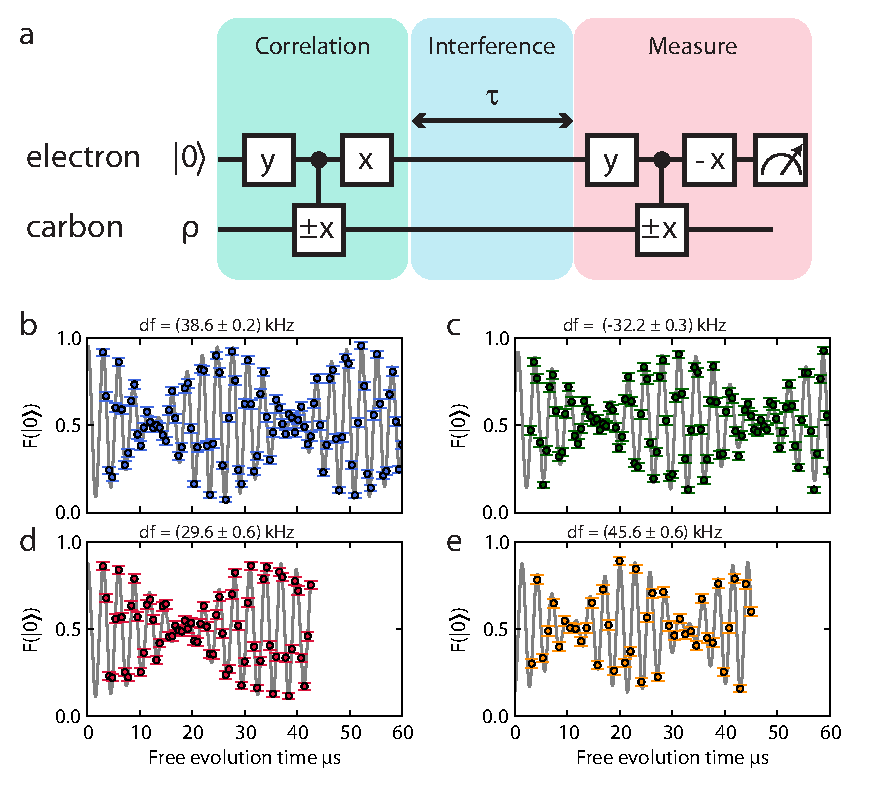
\includegraphics[width=130mm]{Fig2}
	\caption{\label{fig:cdl-fig2} \textbf{Characterization of single $^{13}C$ spins.} (a) Circuit diagram to determine $\omega_0$ and $\omega_1$ of individual $^{13}C$ spins via the electron spin. The conditional gates on the carbon spin are implemented using resonant dynamical decoupling techniques as explained in the main text. Because the evolution of the carbon spin is correlated with an eigenstate of the electron spin during the interference, a coherent signal can be observed even for $\tau \gg T^{*}_{2,electron}$ = (4.18 $\pm$ 0.01) $\mu$s (b)-(e) The resulting interference signal measured for four individual $^{13}C$ spins near a single NV-center. Grey lines are fits to the data with function $F = \frac{A}{2}\cos(\omega_0 \tau +\phi_0) + \frac{B}{2}\cos(\omega_1 \tau + \phi_1)$. We find $\omega_0$ /2$\pi$ = (326.0 $\pm$ 0.2), (325.9 $\pm$ 0.2), (325.1 $\pm$ 0.5), (325.9 $\pm$ 0.4) kHz (b-e), consistent with the gyromagnetic ratio of a $^{13}C$ spin in a field of (303 $\pm$ 1) G.  For the second frequency component we find $\omega_1$ /2$\pi$ = (364.6 $\pm$ 0.1), (293.7 $\pm$ 0.2), (354.7 $\pm$ 0.5), (371.5 $\pm$ 0.4) kHz. The data is taken with 500 repetitions per data point and the error bars correspond to one standard deviation.}
\end{figure*}

Because the hyperfine interaction is determined by the specific position of each nuclear spin relative to the NV center, the resonance condition for $\tau$ is different for each nuclear spin. We can thus characterize the nuclear spin environment\cite{Taminiau_Phys.Rev.Lett._2012} by preparing the electron in a superposition state and measuring the phase that is acquired when sweeping $\tau$. Here we select four individual $^{13}C$ spins to study in more detail, and design controlled gates following Taminiau et al.\cite{Taminiau_NatNano_2014}.

The nuclear spin dynamics are characterized by the nuclear spin precession frequencies $\omega_0$ and $\omega_1$  corresponding to the electron spin being in $m_s = 0$ and $m_s = 1$, respectively (see also Methods). To directly determine the frequencies $\omega_0$,  $\omega_1$ and $df = ( \omega_1 − \omega_0 )/2 \pi$  for each of the four nuclear spins we perform the experimental sequence\cite{Laraoui_NatCommun_2013} shown in Fig. \ref{fig:cdl-fig2}a. The electron is prepared in state $\rho_{0,e} = \ket{0}\bra{0}$, whereas the nuclear spin state is un-polarized (mixed state $\rho_{m.C} = (\ket{0}\bra{0} + \ket{1}\bra{1})/2$ ). The first set of gates correlates the electron state with the X-projection of the nuclear spin state, so that the state is $\rho_{0,e} \otimes \rho_{x,C} + \rho_{1,e} \otimes \rho_{-x,C}$ , with $\rho_{\pm X,C} = \ket{\pm X}\bra{\pm X}$ and  $\ket{\pm X} = (\ket{0}_C \pm \ket{1}_C)/\sqrt{2}$. The controlled nuclear spin rotations are realized by the pulse sequences described above, with $\tau$ resonant for that specific spin. Second, the nuclear spin evolves freely, either with $\omega_0$ or with $\omega_1$, depending on the electron state. Finally the phase accumulation of the nuclear spin is measured by correlating it to the electron spin before reading out the electron spin. 

The beating observed in the signal directly yields the frequency difference df and therefore the additional phase picked up due to the time the electron spent in $m_s = + 1$.   For the four spins we find $df = (29.6 \pm 0.6), (-32.2 \pm 0.3) (38.6 \pm 0.2)$ and $ (45.6 \pm 0.6) $  kHz respectively.  These values show that several nuclear spins with coupling strengths between approximately 20-50 kHz are readily available in diamond samples with a natural abundance of $^{13}C$.

\section{Modeling the dephasing of a carbon spin during entanglement generation}

We analyze the performance of $^{13}C$ spins as quantum memory in the context of  the  heralded entanglement protocol proposed by Barrett and Kok\cite{Barrett_Phys.Rev.A_2005}, which was implemented by Bernien et al.\cite{Bernien_Nature_2013}. The protocol is based on the creation of spin-photon entanglement at both nodes, followed by two-photon interference and measurement of these photons. The protocol is probabilistic since it is susceptible to photon loss. Importantly, successful generation of entanglement is heralded by the detection of the two photons and thus the sequence can be repeated until successful. 

Spin-photon entanglement is created using the following sequence (Fig. \ref{fig:cdl-fig3}a). The electron spin is prepared in state $\ket{0}_e$ by optical pumping (Fig. \ref{fig:cdl-fig1}d). Using microwaves the electron spin is then brought in a coherent superposition. Next, the NV center is optically excited with a short laser pulse that is only resonant if the spin is in state $\ket{0}_e$. Spontaneous emission generates a photon that is entangled with the state of the spin: $\ket{\Psi} = (\ket{0}_e \ket{1}_p +\ket{1}_e \ket{0}_p)/\sqrt{2}$  where $\ket{1}_p$ ($\ket{0}_p$)  denotes the presence (absence) of a photon. The goal is that the nuclear spin memory reliably stores quantum states during many repetitions of this sequence.

 \begin{figure*}
	\centering
	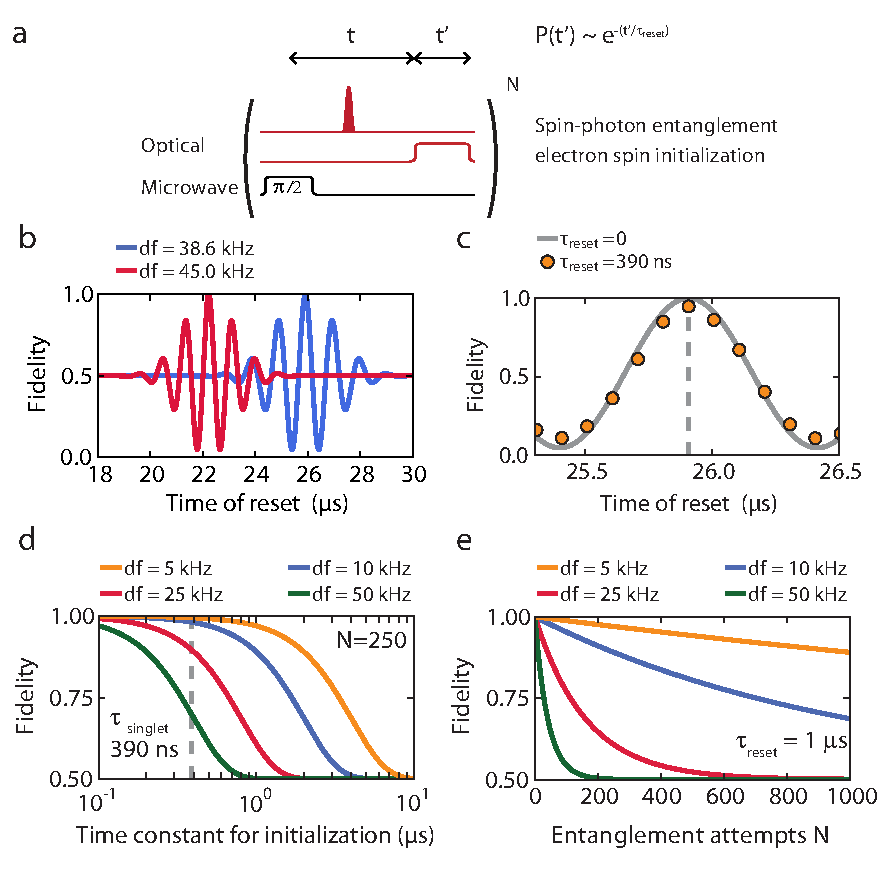
\includegraphics[width=130mm]{Fig3}
	\caption{\label{fig:cdl-fig3} \textbf{Simulations of the dephasing of a $^{13}C$ spin quantum memory while generating entanglement. } (a) Diagram for the protocol to create spin-photon entanglement. (b) Simulations of the fidelity for different $^{13}C$ spins after \textit{N} = 50 repetitions of the protocol, assuming that the reset is instantaneous ($t^{\prime}$ = 0, formula \ref{eq:CDL-deph} of main text). The initial state of a carbon spin can be perfectly preserved by choosing the time between the $\pi$/2-pulse and the reset to \textit{t} = 2$\pi$ /$d \omega$. (c) The effect of the spin pumping process on the fidelity of the memory after \textit{N} = 50 repetitions. Orange dots are a Monte-Carlo simulation where for every electron spin reset, a time $t^{\prime}$ is drawn from an exponential probability distribution with $\tau_{reset}$ = 390 ns. Grey line is a comparison with an ideal reset. $d \omega$ = (2$\pi$) 38.6 kHz. (d) Dependence of the memory fidelity on the characteristic reset time $\tau_{reset}$ using formula \ref{eq:CDL-deph_an}. (e) Dephasing of the memory as a function of entanglement attempts for different coupling strengths, fixing  $\tau_{reset}$ = 1 $\mu$s.}
\end{figure*}



The performance of a quantum memory can be characterized by its ability to store an unknown quantum state $\ket{\psi} = \alpha \ket{0}_C + \beta e^{i \phi}\ket{1}_C$. During the spin-photon entanglement sequences the phase $\phi$ of the nuclear spin state is affected in two ways. First, when the emitted photon is lost (heralding fails), the electron spin state is randomly projected into either $\ket{0}_e$ or $\ket{1}_e$ resulting in nuclear spin evolutions with $\omega_0$ or $\omega_1$, respectively. Second, before the next repetition, the electron spin is reset by optical pumping, a stochastic process that introduces a distribution of spin flip times. These two effects are now analyzed separately.

After a single round of optical excitation that generates spin-photon entanglement, the electron spin is projected into an unknown eigenstate if the photon is lost. The carbon spin acquires a phase $d \omega t$ if the electron is projected in $\ket{1}_e$, where $d \omega = 2 \pi df$ and \textit{t} the time at which the reset is applied. When this process is repeated \textit{N} times, the number of times \textit{k} that the electron is projected in $\ket{1}_e$ is given by a binomial distribution and the final state fidelity \textit{F} of the carbon spin state is given by:

\begin{equation}\label{eq:CDL-deph}
F = \frac{1}{2} + \frac{1}{2^{N+1}} \sum_{k=0}^{N} \binom{N}{k} \cos \lbrack k d \omega t \rbrack
\end{equation}

where the electron spin reset is taken to be instantaneous and we only consider the initial memory state is $\ket{\psi} = (\ket{0}_C + \ket{1}_C/\sqrt(2)$, which is most sensitive to dephasing. Fig. \ref{fig:cdl-fig3}b shows the calculated fidelity as a function of the time \textit{t}, for two carbon spins that were identified in Fig. \ref{fig:cdl-fig2}. For each carbon spin there is a unique condition at \textit{t} =2$\pi$ /$d \omega$, for which the phase is independent on the electron state resulting in \textit{F} = 1. Note that in the full entanglement protocol\cite{Bernien_Nature_2013,Barrett_Phys.Rev.A_2005} an electron $\pi$-pulse is applied between rounds of excitation, so that this phase difference can be cancelled for all \textit{t}. 


In reality the reset of the electron spin by spin pumping is a stochastic process involving multiple transitions to the optically excited state as well as mixing between multiple excited states. Here we model the dynamics of this process as an exponential distribution  $e^{- \frac{ t^{\prime} } {\tau_{reset} } }$  with a characteristic time $\tau_{reset}$.  In Fig. \ref{fig:cdl-fig3}c we compare the results of a monte-carlo simulation that includes the probabilistic reset time $t^{\prime}$ for $\tau_{reset}$ = 390 ns with the curve of equation \ref{eq:CDL-deph}. As expected the same behavior is observed, but the maximum fidelity is reduced since the stochastic reset leads to dephasing of the carbon spin. 

To analyze the effect of the electron spin reset on the nuclear spin in detail we now assume that  \textit{t} = 2$\pi$ $d\omega$ which allows us to derive an analytical expression for the fidelity of the carbon spin (see methods for the derivation of this result): 

\begin{equation}\label{eq:CDL-deph_an}
F = \frac{1}{2} + \frac{1}{2^{N+1}}\left(1 + e^{-\frac{1}{2}\tau_{reset} ^2 d\omega^2}\right)^N.
\end{equation}

In Fig. \ref{fig:cdl-fig3}d we plot the resulting memory fidelity after 250 entanglement repetitions versus the reset constant $\tau_{reset}$, for different values of \textit{df}. Although for an instantaneous reset ($\tau_{reset} \to 0$) the state can be perfectly preserved, a finite uncertainty in the reset time constant reduces the fidelity, with the effect being stronger for higher coupling strengths df. A natural lower limit to the reset time $\tau_{reset}$ is the slowest decay rate involved in the spin pumping process. For the NV center this is expected to be the singlet lifetime $\tau_{singlet} \approx$ 390 ns\cite{Doherty_PhysicsReports_2013}.  For this value, Fig. \ref{fig:cdl-fig3}d predicts that for coupling strengths of \textit{df} < 10 kHz the state can be preserved with a fidelity of > 98 \% even after 250 entanglement attempts. 

The reset constants currently reported in the literature are approximately 1 $\mu$s \cite{Bernien_Nature_2013}. In Fig. \ref{fig:cdl-fig3}e we plot the fidelity as a function of number of entanglement attempts for $\tau_{reset}$ = 1 $\mu$s. These calculations predict that 25 repetitions of the entanglement protocol will yield a fidelity of 90.3 \% for the lowest coupling strength found in Fig. \ref{fig:cdl-fig2}, which would already provide significant speed advantages in establishing entanglement links\cite{Campbell_Phys.Rev.Lett._2008}. For coupling strengths \textit{df} < 10 kHz, hundreds of repetitions become feasible. Such lower coupling strengths are available in isotopically purified diamonds\cite{Maurer_Science_2012}.

We emphasize that the model presented here does not include the detailed excited state dynamics of the spin pumping process. We expect that averaging over rapid spin flips and time spent in states with zero spin projection during these dynamics will further reduce actual dephasing. We therefore expect that our analysis sets a lower bound for the number of possible repetitions.

We have modelled the dephasing of nuclear spins quantum memories coupled to an NV electron spin that is repeatedly used to establish spin-photon entanglement. We find that nuclear spins with weak hyperfine couplings (20-50 kHz) are readily available in natural abundance diamonds. Our analysis shows that these spins can be used to store quantum states during 25 entanglement attempts with a fidelity of 90.3 \%, while nuclear spins in isotopically purified samples with coupling strengths below 10 kHz can even enable hundreds of repetitions. These results demonstrate that nuclear spins with weak hyperfine coupling strengths are promising quantum memories for quantum networks providing a route towards entanglement distillation and quantum repeaters.

\section{Methods}
We take the limit of $\gamma_C B \gg A_{\perp}$ (with $A_{\perp}$  the hyperfine component perpendicular to the static magnetic field) such that the eigenstates of the $^{13}$C-spin are independent of the electron and the only net effect of the electron-carbon coupling is that the carbon acquires a phase depending on the state of the electron. Choosing the rotating frame of the carbon resonant with the energy splitting for the electron in $\ket{0}_e$, the carbon state will acquire a phase $e^{id\omega t}$ for the electron in $\ket{1}_e$ (with $d \omega$ = 2$\pi$ \textit{df}) and does not evolve otherwise.

We derive an expression for the maximally achievable memory fidelity. The scheme of Fig 3a is repeated \textit{N} times. Phase errors occur if the electron spin has to be reinitialized by pumping it to another spin state. During every execution of the protocol, the electron spin is projected into $\ket{0}_e$ or $\ket{1}_e$ with equal probability. The probability for \textit{k} repumping events is then given by a binomial distribution

\begin{equation}
P_{ek} = \frac{1}{2^N}\binom{N}{k}
\end{equation}

Every time the electron is reset from $\ket{1}_e$ into $\ket{0}_e$ the memory spin will pick up a random phase $\delta \theta = d \omega (t^{\prime} - \tau_{reset})$ which is given by the difference between energy levels of the carbon spin conditional on the electron spin $d \omega$ and the deviation $(t^{\prime} - \tau_{reset})$ from the mean repumping time. The overall acquired phase for \textit{k}  repumping events is then the sum of the individual random phases. The fidelity with the initial memory state after \textit{N} repetitions is thus given by

\begin{equation}
F_k = \frac{1}{2}\left(1+\cos \left[\sum_{k=0}^N \delta \theta_k\right]\right)
\end{equation}

Under the assumption that the distributions for all repumping events are independent the problem can be seen as a random walk in accumulated repumping time. Each step of this random walk is then exponentially distributed around the mean repumping time $\tau_{reset}$. The probability distribution of the summed repumping time is given by\cite{Akkouchi_CCMS_2008}

\begin{equation}
P(t^{\prime}) = \frac{t'^{k-1}}{\tau_{reset}^k(k-1)! }e^{-t^{\prime}/\tau_{reset}} \approx \frac{1}{\sqrt{2\pi}\sigma}e^{-\frac{(t^{\prime}-\mu)^2}{2\sigma^2}}
\end{equation}


where we use the central limit theorem to approximate this distribution by a normal distribution with width $\sigma = \tau_{reset} \sqrt{k}$ and mean $\mu = \tau_{reset} k$ , as we are interested in solutions for a large number of repumping events. The expected fidelity after \textit{N} experimental runs is calculated by summing over the probability distributions for the electronic state and the corresponding accumulated repumping time

\begin{eqnarray}
F_N & = & \sum_{k=0}^N  P_{ek} \int F_k\, P(t^{\prime})\, dt^{\prime} \nonumber \\
& = & \frac{1}{2} + \frac{1}{2} \sum_{k=0}^N P_{ek} e^{-\frac{1}{2}k\tau_{reset}^2 d \omega^2} \nonumber \\
& = & \frac{1}{2} + \frac{1}{2^{N+1}}\left(1 + e^{-\frac{1}{2}\tau_{reset}^2 d \omega^2}\right)^N.
\end{eqnarray}

\newpage
\bibliographystyle{../thesis}
\bibliography{cdl}



\graphicspath{{./ch_carbon_dephasing_purified/figures/}}


\chapter{Storing a quantum state during optical excitation of a quantum network node}
\label{ch:CDP}

\begin{center} 
    \vspace{-1cm} {M.S.~Blok, K. ~van Bemmelen, N.~Kalb, A.~Reiserer, T.H.~Taminiau and R.~Hanson} 
\end{center}

\vspace{0.5cm} 

The ability to locally store a quantum state in a quantum network node while establishing entanglement with a distant node is a crucial prerequisite for implementing entanglement distillation, purification and quantum repeater protocols\cite{Bennett_Phys.Rev.Lett._1996,Campbell_Phys.Rev.Lett._2008,Briegel_Phys.Rev.Lett._1998,Childress_Phys.Rev.Lett._2006}. For quantum network nodes based on NV centers in diamond, nearby $^{13}$C-spins are a prime candidate for such a quantum memory. The challenge is that these nuclear spins have a constant coupling to the optically active electron spin, resulting in possible dephasing of the stored state when the electron is reset multiple times as required for generating remote entanglement. In chapter \ref{ch:CDL} we discussed an analytical model to describe this process and found that nodes with low electron-nuclear coupling strength and fast electron reset are expected to provide the best performance. Here we present preliminary experimental results to test our model in an isotopically purified sample where $^{13}$C-spins with coupling strengths of < 1 kHz can be located and controlled. We find that multiple resets of the electron spin indeed induce dephasing of the nuclear-spin quantum memory and that this process can be suppressed by reducing the electron reset time. While the data qualitatively agrees with our model, the observed dephasing rate is faster than predicted indicating that we are limited by an additional decoherence process. Nonetheless our results show that a $^{13}$C-spin allows for the storage of a quantum state during 200 repetitions with very little loss of fidelity ($99 \%$ fidelity with initial state).
\clearpage

Here we investigate the ability of a weakly coupled $^{13}$C-spin to store a quantum state while optically addressing the electron spin to generate remote entanglement (as presented in chapter \ref{ch:LDE}). Since this protocol \cite{Barrett_Phys.Rev.A_2005,Bernien_Nature_2013} is inherently probabilistic it must be repeated many times until success, requiring the electron spin to be reset before each repetition. Because the exact time of our reset method is uncertain (the optical pumping is a stochastic process) and electron-nuclear interaction is constant, this can induce dephasing of the nuclear spin memory. From the simulations presented in chapter \ref{ch:CDL} we conclude that this dephasing process can be suppressed by using relatively distant $^{13}$C-spins with low hyperfine coupling and implementing a fast reset that minimizes the time-uncertainty. To locate distant $^{13}$C-spins we use an isotopically purified diamond (0.01 $\%$ $^{13}$C) and show that we can control nuclear spins with a hyperfine coupling constant in the order of $\sim$ 200 Hz. We characterize the reset timescale by varying the time and the power of the repumping laser pulse. Finally we measure the dephasing of the nuclear spin as a function of number of times that the electron spin is reinitialized.

\section{Controlling a weakly coupled $^{13}$C-spin in isotopically purified diamond.}

We detect weakly coupled $^{13}$C-spins in the vicinity of an NV center via the electron spin using dynamical decoupling spectroscopy\cite{Taminiau_Phys.Rev.Lett._2012,Zhao_NatNano_2012,Kolkowitz_Phys.Rev.Lett._2012}. In Fig. \ref{fig:cdp-fig1}a we vary the time between $N = 128$ equally spaced $\pi$-pulses on the electron initially prepared in an equal superposition and plot the probability of recovering $m_s = 0$ after a final $\pi$/2-pulse. The observed periodical collapses\cite{Childress_Science_2006} are well explained by the interaction of the electron spin with a $^{13}$C-spin bath in a magnetic field of 22.7 $G$. We align the magnetic field along the quantization axis of the NV-center by minimizing the average of the $m_s = 0 \rightarrow -1$ and $m_s = 0 \rightarrow +1$ transitions. From these measurements we find a magnetic field $B_z = (22.5 \pm 0.1) $ G and $B_x = (2.4 \pm 2) $ G.

In a higher resolution measurement around the second collapse (Fig. \ref{fig:cdp-fig1}b) we observe two additional resonances associated with single $^{13}$C-spins. The location and shape of these resonances are determined by the hyperfine parameters of the carbon spin\cite{Taminiau_Phys.Rev.Lett._2012}. By comparing the data with simulations of the electron-nuclear interaction we estimate hyperfine constants of $A_{\parallel,C} = 220$ Hz and $A_{\perp,C} = 200$ Hz ($A_{\parallel,C} = -1.02$ kHz and $A_{\perp,C} = 190$ Hz) as plotted in red (green). In comparison, previous experiments have demonstrated control of strongly coupled $^{13}$C-spins with interaction strengths between $\sim$ 100 - 1 MHz \cite{Jelezko_Phys.Rev.Lett._2004,Dutt_Science_2007,Pfaff_NatPhys_2013,Neumann_Science_2008} and weakly coupled nuclear spins in the order of 50-30 kHz \cite{Taminiau_NatNano_2014} in natural abundance samples. In isotopically purified samples, manipulation of a strongly coupled 2.6 kHz $^{13}$C-spin was demonstrated\cite{Maurer_Science_2012}.

 \begin{figure*}
	\centering
	\includegraphics[width=130mm]{Fig1}
	\caption{\label{fig:cdp-fig1} \textbf{} (a) Dynamical Decoupling spectroscopy of the $^{13}$C-spin bath. Grey lines are the expected collapses of the signal due to interaction with the $^{13}$C-spin bath. They occur at $\tau_k = \frac{\pi(2k-1)}{2\omega_L}$, with $k = 1,2,3...$ the order of the resonance and $\omega_L$ the larmor frequency of the $^{13}$C spins.(b) Two $^{13}$C-spins can be identified, red (green) line is a simulation of the resulting signal for the interaction with a single spin with hyperfine constants of $A_{\parallel,C} = 220$ Hz and $A_{\perp,C} = 200$ Hz ($A_{\parallel,C} = -1.02$ kHz and $A_{\perp,C} = 190$ Hz), plotted in red: carbon 1 (green: carbon 2). (c) Free induction decay of carbon 1 with and without repetitive reset }
\end{figure*}

We control an individual $^{13}$C-spin by applying $\pi$-pulses to the electron spin and by choosing the time between the pulses on resonance with the electron-nuclear coupling \cite{Taminiau_Phys.Rev.Lett._2012,Taminiau_NatNano_2014}. This results in a rotation of the nuclear spin conditional on the initial electron spin state, hence by choosing the initial state of the electron we can construct one-, and two-qubit gates. The $^{13}$C spin is initialized and measured by entangling the electron and nuclear spin and subsequent readout of the electron spin. In Fig. \ref{fig:cdp-fig1}c we show a Ramsey measurement of carbon 1. By measuring the precession frequency of the carbon spin depending of the electron spin state we find the frequency difference $df = (227 \pm 6)$Hz. This parameter is expected to be relevant for the nuclear spin dephasing rate upon repetitive reset of the electron spin as discussed in chapter \ref{ch:CDL}. The free induction decay of the nuclear spin is measured for the electron spin in an eigenstate (Fig. \ref{fig:cdp-fig1}c right panel) and when the electron spin is reset every $\sim$ 12 $\mu$s (Fig. \ref{fig:cdp-fig1}c left panel). By comparing the resulting decoherence times $T_{decay}$, we find that repetitive reset of the electron spin reduces the coherence time roughly with a factor of 50. From equation \ref{eq:CDL-deph_an} we find the product of the frequency difference $df$ and the reset time $\tau_{reset}$ to set the timescale of dephasing. We therefore now characterize the optical spin-pumping process of the electron.



\section{Fast optical reset of the electron spin.}

To measure the time required to reset the electron spin we prepare $m_s= -1$ and plot the probability to prepare $m_s = 0$ after applying an optical pulse on the $E^{\prime}$ transition for a variable time (Fig. \ref{fig:cdp-fig2}a). We find that the data can be fitted to a double exponential function, consistent with previous measurements of the fluorescence during optical repumping on $E_y$ and $A_1$\cite{Bernien_Nature_2013}. This indicates that the spin pumping process involves transitions to multiple levels in the excited state, such as the meta-stable singlet state. In Fig. \ref{fig:cdp-fig2}b we plot the largest of the two time constants obtained from the fits in Fig. \ref{fig:cdp-fig2}a as a function of laser power. For low laser power the reset time is likely to be limited by the excitation rate to the excited state. Increasing the laser power significantly reduces the reset time until it saturates around 200 ns, which could indicate that here the spin pumping is limited by the lifetime of the meta-stable singlet state \cite{Doherty_PhysicsReports_2013}.

For a 500 nW repump pulse we find that the electron spin can be reset within a microsecond, with a characteristic time constant $\tau_{reset} = (220 \pm 27) $ ns. Apart from reducing dephasing of the nuclear spin due to electron spin flips, this also allows for an increased entanglement generation rate since the repetition rate of the experiments presented in chapter \ref{ch:LDE} was limited by the 5 $\mu$s repump pulse. However in figure $\ref{fig:cdp-fig2}$ the electron spin is reset once, while the heralded entanglement protocol requires repetitive initialization steps. We find that for repetitive electron initialization with a 500 nW pulse there is a significant probability to ionize the NV center after several hundreds of repetitions. We therefore now analyze the carbon dephasing for a maximum laser power of 100 nW where no significant ionization is observed.

 \begin{figure*}
	\centering
	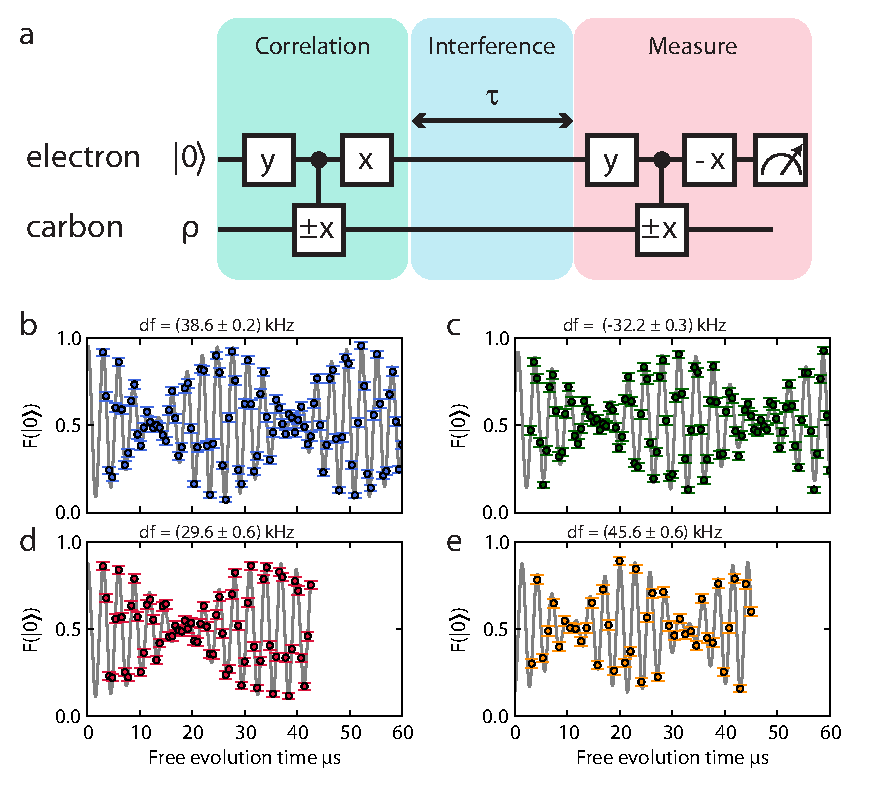
\includegraphics[width=130mm]{Fig2}
	\caption{\label{fig:cdp-fig2} \textbf{Reset of the electron spin} (a) Measurement of the timescale of the reset process. Plotted is the probability of preparing $m_s = 0$ after preparing $m_s = -1$ as a function of repump time and power. Solid lines are fits to the function $S = o - A e^{-\frac{x-x_o}{\tau_{reset}}}-(1-A) e^{-\frac{x-x_o}{\tau_{reset,2}}}$ (b) Largest of the two fitted time constant of the reset process as a function of reset power.}
\end{figure*}

\section{Dephasing of a carbon spin upon optical excitation of the electron spin.}

 We demonstrate the robustness of the carbon spin quantum memory by measuring its ability to store a coherent quantum state while performing the local operations for generating heralded entanglement on the electron spin (Fig. \ref{fig:cdp-fig3}). We prepare carbon spin 1 in a maximum superposition $\ket{\psi}=(\ket{0}_C + \ket{1}_C)/\sqrt{2}$ and perform state tomography after a variable number of protocol repetitions (sequence on electron spin is ($\pi/2 - \pi -$ reset)$^N$, see Fig. \ref{fig:LDE-fig1-protocol}). We omit the two optical $\pi$-pulses to generate spin-photon entanglement. We expect their influence on the carbon spin to be negligible since they effectively perform a measurement of the electron spin which in this case can be incorporated into the reset.
 \begin{figure*}
	\centering
	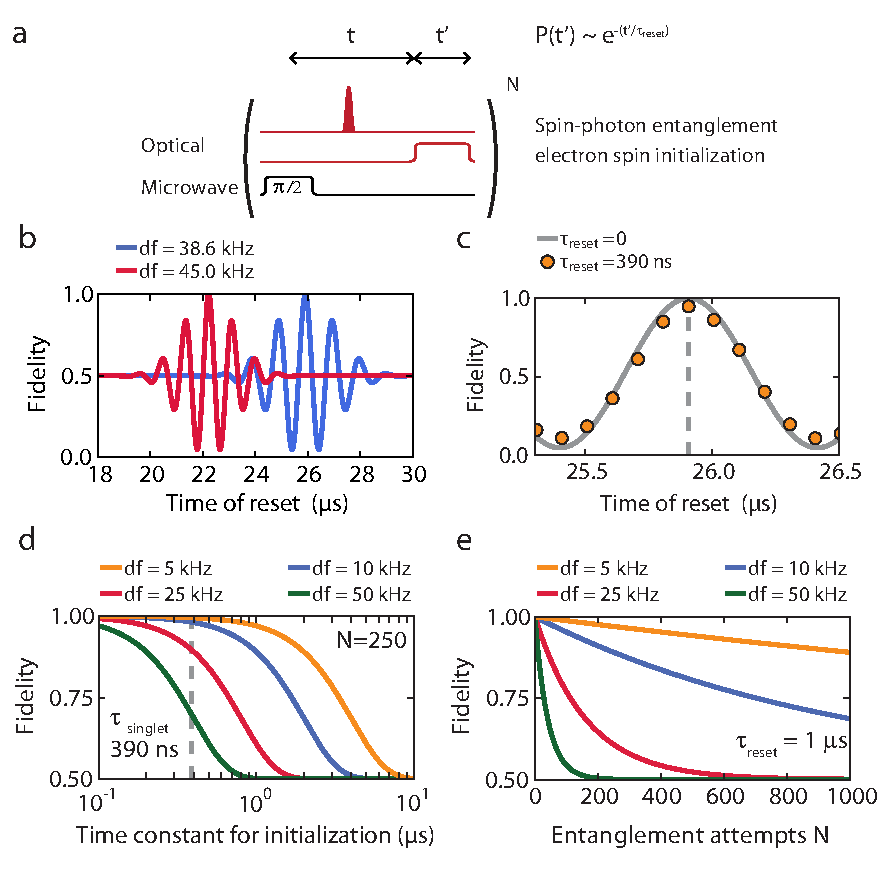
\includegraphics[width=130mm]{Fig3}
	\caption{\label{fig:cdp-fig3} \textbf{} (a) Tomography of carbon spin 1 initially prepared in a superposition as a function of number of repetitions of the heralded entanglement protocol. The repumping pulse is applied for 20 $\mu$s with a power of 100 nW, the time before and after the microwave $pi$-pulse is 200 ns. (b) Dephasing of the carbon spin for different repumping powers, with the same repump time and interpulse delay as in (a). Inset: the decay constants obtained from a fit to the data in (b) as a function of $\tau_{reset}$ for that laser power. }
\end{figure*}

In Fig. \ref{fig:cdp-fig3}a we show that after 200 repetitions the initial state is almost perfectly recovered for 100 nW repump power ($\tau_{reset} = (870 \pm 100)$ ns). The oscillation in the XY-plane of the Bloch sphere is due to the larmor precession of the carbon spin. In a realistic protocol where the number of required repetitions is probabilistic, this oscillation can be correct with real-time feedback. We therefore take the quadratic sum of the expectation values $<X>_C$ and $<Y>_C$ as a figure of merit and find that this quantity is preserved with a fidelity of $(99 \pm 1) \%$ after 200 repetitions.

Strikingly when we plot the full decay curve (Fig. \ref{fig:cdp-fig3}b) we find that the signal is best fitted with a Gaussian as opposed to an exponential function as expected from equation \ref{eq:CDL-deph_an}. Furthermore, while the measured decay constants for variable reset duration (inset of \ref{fig:cdp-fig3}b) can be fitted to the model, they are two orders of magnitude smaller than expected from the independently measured reset time and coupling constant. Since the decoherence rate is also faster than the intrinsic $T_2^{*}$ of the carbon spin, we conclude that the electron reset induces an additional decoherence process that is not included in our model. One hypothesis is that the perpendicular component of the hyperfine interaction ($A_{perp}$, neglected in chapter \ref{ch:CDL}) induces dynamics that lead to a $T_1$-type of decay. This can be verified by measuring the decay of an eigenstate of the carbon spin upon repumping the electron spin. Secondly the model simplifies the spin pumping process which in reality involves multiple transitions in the excited state. 

These experiments establish weakly coupled carbon spins as promising candidates for a memory in a quantum network node based on NV centers. Although further measurements are required to understand the limiting decoherence mechanism, the ability to store a quantum state for hundreds of repetitions can significantly improve the rate at which remote entanglement is established. These results show that in an isotopically purified diamond it is possible to preserve the coherence of a carbon spin during 200 repetitive resets of the electron spin. This is the maximum number of consecutive attempts to generate remote entanglement in previous experiments with NV centers\cite{Bernien_Nature_2013,Pfaff_Science_2014}. However, in protocols that aim to improve the entangling rate by using a quantum memory, the overhead associated with gates on the memory needs to be taken into account. Finding an optimal carbon spin for a quantum memory therefore poses a trade-off between its robustness against optical excitation of the electron spin and the gate-time, since the minimum time required to perform a gate between the nuclear spin and the electron spin is inversely proportional to the coupling strength. Furthermore, all errors in preparing and storing a state in the carbon spin will propagate to the resulting remote entanglement fidelity and therefore the carbon manipulation needs to be improved. In future work the incorporation of a quantum memory in a local node could be combined with the experiments presented in chapter \ref{ch:LDE} to demonstrate entanglement purification\cite{Campbell_Phys.Rev.Lett._2008} and eventually quantum repeaters \cite{Briegel_Phys.Rev.Lett._1998}.

\clearpage
\bibliographystyle{../thesis}
\bibliography{cdp}




\graphicspath{{./ch_conclusion_and_outlook/figures/}}

\chapter{Conclusions and outlook}
\label{ch:conclusion}

\begin{center} 
    \vspace{-1cm} {M.S. ~Blok} 
\end{center}

Future quantum technologies have the potential to have great impact on the fields of computation, communication and metrology. The work presented in this thesis capitalizes recently developed low temperature control techniques of the NV center in diamond to study quantum measurements and implement real-time feedback protocols. This transition from open-loop control to feedback control experiments will aid the development of diamond-based quantum technologies. In this chapter we give an overview of the main results and conclusions and provide an outlook for future research directions.
\clearpage

\section{Summary}
The results of this thesis can be summarized as follows.
\begin{itemize}

  \item A variable-strength measurement of the nitrogen spin of an NV center can be implemented via the electron spin. The backaction of sequential variable-strength measurements can be used to manipulate the nitrogen spin when digital feedback is incorporated.

  \item The advantage of adaptive frequency estimation protocols using the electron spin of a NV center is that fewer measurements are required to reach the same sensitivity compared to the best non-adaptive protocols. When overhead is included in the analysis this results a more accurate estimation at any fixed measurement time.

  \item Two electron spins in spatially separated diamonds can be entangled by performing a joint measurement of photons originating from the two NV centers. 

  \item Remote entanglement between two NV centers established via an heralded protocol can be used to unconditionally teleport the state of a nuclear spin to a distant electron spin.

  \item Weakly-coupled carbon spins in an isotopically purified diamond can maintain their coherence even after 200 repetitive resets of the electron spin.
  
\end{itemize}

This thesis reports the first experiments with spins in diamond where measurement outcomes are used as input for subsequent control operations thereby closing the loop between measurement and control. Furthermore they establish NV centers as a leading platform for building quantum networks.  Other systems are of course being developed in parallel and like spins in diamond each has their advantages and disadvantages. Recent advances include generation of remote entanglement between trapped ions \cite{Moehring_Nature_2007} and atoms\cite{Hofmann_Science_2012,Ritter_Nature_2012} and atomic ensembles\cite{Chou_Nature_2005} and the implementation of real-time feedback protocols using superconducting circuits\cite{Vijay_Nature_2012,Riste_Nature_2013} and photons \cite{Gillett_Phys.Rev.Lett._2010,Sayrin_Nature_2011}. The following sections will provide an outlook for future research directions with NV centers in diamond.

\section{Quantum Information Processing with NV centers in diamond}
A scalable solution for implementing quantum information technology with NV centers remains a long-term goal and making predictions of how this technology can be developed unavoidably contains some speculation. However it is possible to identify short-term challenges and provide possible solutions to overcome them. The demands on the system will depend on the application. A quantum computer will probably require a vast amount of physical qubits, while a big challenge for a quantum internet lies in entangling nodes with a relatively small amount of qubits over large distances. I will first discuss the challenge of locally scaling up the number of qubits and then proceed to connecting remote quantum nodes.

One challenge that can be overcome using real-time feedback is to protect quantum states against errors. A promising way to deal with noisy operations is to redundantly encode a logical qubit in multiple physical qubits and detect errors by measuring joint properties of the physical qubits without destroying the logical state. When an error is detected it can be corrected with real-time feedback based on the outcome of the multi-qubit measurements. This measurement based quantum error correction has recently been implemented using three weakly coupled $^{13}$C-spins and the quantum non-demolition measurement of the electron spin presented in chapter \ref{ch:AMC} to correct for one type of error\cite{Cramer_arXiv_2015}. The next step is to increase the number of encoding qubits to protect against arbitrary errors and to improve the gate fidelities to reach the scalability threshold. Higher gate fidelity could be achieved using asymmetrical dynamical decoupling sequences\cite{Casanova_arXiv_2015} or via numerical optimization \cite{Liu_NatCommun_2013,Dolde_NatCommun_2014}. Using dynamical decoupling spectroscopy techniques it has been demonstrated that six individual carbons can be identified\cite{Taminiau_Phys.Rev.Lett._2012}. It is still an open question how many carbon spins can be controlled with the electron spin. However it seems impractical to control a large amount of carbon spins via a single electron spin because all operations need to be applied sequentially and optimizing gates will become increasingly difficult for larger systems.

A promising way to engineer a scalable system is to adopt a modular approach where individual nodes consisting of one electron spin and a few nuclear spins are entangled using the optical interface. A recent proposal to implement the surface code using this quantum network architecture showed that the error thresholds of the entanglement generation can be reasonably high (10\%) if the local error rates for initialization, control and measurement are in the order of a percent\cite{Nickerson_NatCommun_2013}. For this approach the heralded entanglement protocol as presented in chapter \ref{ch:LDE} would have to be improved, given the current entanglement rate of 1/250 s$^{-1}$. To this end the NV center can be placed in a fiber-based micro cavity to enhance the photon collection efficiency and the emission in the zero phonon line via the Purcell effect\cite{Kaupp_Phys.Rev.A_2013,Albrecht_Phys.Rev.Lett._2013,Janitz_arXiv_2015}. When a highly connected quantum network is realized it would also lend itself for performing measurement-based quantum computing\cite{Raussendorf_Phys.Rev.Lett._2001,Benjamin_Laser&Photon.Rev._2009} where highly entangled graph states are first created and then the computation is performed by adaptive measurements.

To increase the separation between nodes in a quantum network for quantum communication one needs to overcome the optical losses. For photons emitted in the zero phonon line (wavelength 637 nm) the attenuation in an optical fiber is in the order of 12 dB/km. In a recent result entanglement over a distance of 1.3 km between two NV centers has been demonstrated\cite{Hensen_arXiv_2015}. In this experiment the entanglement rate was severely reduced by losses in the fiber. One way to overcome this is to downconvert the photons to telecom wavelength as was recently demonstrated with quantum dot emission\cite{DeGreve_Nature_2012,Zaske_Phys.Rev.Lett._2012}. Furthermore by employing weakly coupled nuclear spins as memories, entanglement purification\cite{Campbell_Phys.Rev.Lett._2008} and quantum repeater protocols\cite{Briegel_Phys.Rev.Lett._1998} can improve the efficiency of probabilistic entanglement generation.

\section{Single spin sensors}
Employing NV centers in diamond as quantum sensors \cite{Taylor_NatPhys_2008,Schirhagl__2014} has gained a lot of interest since the electron spin is sensitive to many physical quantities like as temperature\cite{Acosta_Phys.Rev.Lett._2010,Toyli_PNAS_2013}, strain\cite{Ovartchaiyapong_NatCommun_2014} and electric and magnetic fields\cite{Taylor_NatPhys_2008,Dolde_NatPhys_2011} with very high spatial resolution. There are several methods to bring the NV center close to the sample. The use of shallow NV centers in bulk diamond has enabled the detection of Johnson noise\cite{Kolkowitz_Science_2015} and spin waves\cite{vanderSar_NatCommun_2015} as well as the magnetic field of biological samples\cite{LeSage_Nature_2013}. Alternatively an NV center can be embedded at the end of a sharp tip that is scanned across the sample\cite{Balasubramanian_Nature_2008,Maletinsky_NatNano_2012,Rondin__2012,Pelliccione_Phys.Rev.Applied_2014,Haberle_NatNano_2015}. Finally NV centers in 
 nanocrystals with a size of a few nanometer can be used and it has been shown that they can be inserted into living cells\cite{Kucsko_Nature_2013}. A severe limitation of shallow NV centers is that surface effects can significantly deteriorate the stability of NV centers since nearby charge can lead to a conversion to NV$^-$ and magnetic noise reduces the coherence times of the spins. It was recently shown that a combination of surface treatment and annealing can improve the optical stability of shallow NV centers in bulk diamond\cite{Chu_NanoLett._2014}.

\section{Fundamentals of quantum mechanics}

Bell \cite{Hensen_arXiv_2015}
reality of wavefunction \cite{Pusey_NatPhys_2012}
weak measurements \cite{Aharonov_Phys.Rev.Lett._1988} toin coss \cite{Ferrie_Phys.Rev.Lett._2014} contextuality \cite{Pusey_Phys.Rev.Lett._2014}
gravitational collapse (\cite{Diosi_PhysicsLettersA_1987}, \cite{Penrose_Phil.Trans.R.Soc.Lond.A_1998}) exp with NV (\cite{Wezel_Proc.R.Soc.A_2012})

\bibliographystyle{../thesis}
\bibliography{conclusions}

\appendix

%\graphicspath{{./ch_adptv_msmnt_magnetometry_SI/figures/}}

\chapter[Adaptive sensing protocols]{Adaptive sensing protocols}
\label{ch:AMMappendix}

\section{Comparison of sensing protocols: numerical simulations}
\label{sec:comparisonprotocols}
In the following, the performances of different single-qubit frequency estimation protocols will be compared through numerical simulations. We will describe and analyse three main sensing algorithms, defined using a pseudo-code in Fig. \ref{fig:ammA1} and Fig. \ref{fig:ammA2}: the limited-adaptive, non-adaptive and optimized-adaptive protocols.

In order to achieve high dynamic range, each estimation sequence consists of \textit{N} different sensing times, multiples of the shortest sensing time $\tau_{min}$ = 20 ns: $\tau_n = 2^{N-n}$ $\tau_{min}$ (n = 1 .. \textit{N}).

After each Ramsey, the electron spin is measured: the result of each detection is indicated in the pseudo-code by the \textbf{Ramsey ($\vartheta$, $\tau$) }function. The input parameters of this function are the sensing time $\tau$ and the phase $\vartheta$ of the second $\pi$/2 pulse. In the simulation code, this function generates a random value $\mu$ ($\mu$ = 0,1), using the python library \textit{numpy.random}, chosen according to the probability distribution [$p_0$, $p_1$ = 1 - $p_0$], where:

\begin{equation}
p_0 = P(0|f_B) = \frac{1+F_0-F_1}{2}+\frac{F_0+F_1-1}{2}e^{-(\frac{\tau}{T_2^*})^2} \cos{[2\pi f_B \tau + \vartheta]}
\end{equation}

$F_0$,$F_1$  are, respectively the readout fidelities for $m_s = 0$ and $m_s = 1$. In the following simulations we use the values: $F_0$ = 0, 0.75, 0.88 or 1.00 ($m_s = 0$), $F_1$  = 0.993 ($m_s$ = 1), $T_2^*$ = 5 $\mu$s  or 96 $\mu$s.

For each Ramsey experiment (indexed here by the label $\ell$), the detection result $\mu_{\ell}$  is used to update the estimation of the magnetic field using Bayes rule: $P(f_B|\mu_1... \mu_{\ell}) \sim P(f_B|\mu_1...\mu_{\ell -1}) P(\mu_{\ell}|f_B)$. This is indicated in the pseudo-code by the function \textbf{Bayesian\textunderscore update (res, $\vartheta$, $\tau$)}.
Due to its periodicity it is convenient to express P($f_B$) in a Fourier series, resulting in the following update rule:

\begin{eqnarray}
p_k^{(\ell)} &=& \frac{1 + (-1)^{\mu_{\ell}}(F_0-F_1)}{2}p_k^{(\ell-1)}\\
\nonumber
& &+e^{-(\frac{\tau}{T_2^*})^2} \frac{(F_0+F_1)-1}{4}[e^{i(\mu_{\ell}\pi+\vartheta_{\ell})}p^{\ell-1}_{k-2^{N-n}}+e^{-i(\mu_{\ell}\pi+\vartheta_{\ell})}p^{\ell-1}_{k+2^{N-n}}]
\end{eqnarray}


Given the periodic nature of phase, the uncertainty is better estimated using the Holevo variance $V_H = (|<e^{i 2 \pi f_B \tau_{min}} >|)^{-2}-1 = ( 2 \pi|p_{(2^{N-n+1}}^{(l-1)} |)^{-2}-1$. The Holevo variance can be minimized by choosing the controlled phase \cite{Cappellaro_Phys.Rev.A_2012}:

\begin{equation}
\vartheta^{ctrl} = \frac{1}{2}\arg\{ p_{2^{N-\ell+1}}^{(\ell - 1)}\}
\end{equation}

One Ramsey experiment per sensing time does not allow to reach the Heisenberg-like scaling since the resulting probability distribution, despite being strongly peaked around the expected value, has very large wings with non-zero probability of outlier outcomes. Outliers, although occurring infrequently, can significantly alter the estimate statistics. While this is true for perfect readout ($F_0$ = $F_1$ = 1) the algorithm performance is  reduced even further by imperfect readout \cite{Said_Phys.Rev.B_2011}. A solution to these problems is to perform $M_n$ Ramsey measurements for each interaction time\cite{Said_Phys.Rev.B_2011}, with $M_n = G + F(n-1)$. 
\begin{figure*}
	\centering
	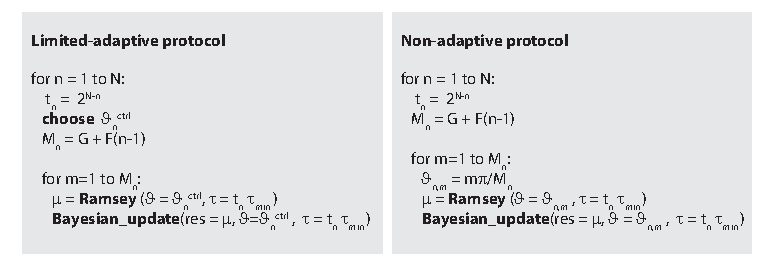
\includegraphics[width=12cm]{algorithms_1}
	\caption{\label{fig:ammA1} \textbf{Pseudo-code for the non-adaptive and limited-adaptive protocols.}}
\end{figure*}

For each protocol it is crucial to find the optimal values for \textit{F} and \textit{G}, given the experimental readout fidelities $F_0$ and $F_1$. The relevant figure of merit is the sensitivity $\eta$, defined as $\eta^2 = V_H T$.
Simulations are performed by running the protocol for 315 different values of the frequency $f_B$, over 315 repetitions for each value. The detection phase $\vartheta$ of the Ramsey is initially set to zero.

\begin{figure*}
	\centering
	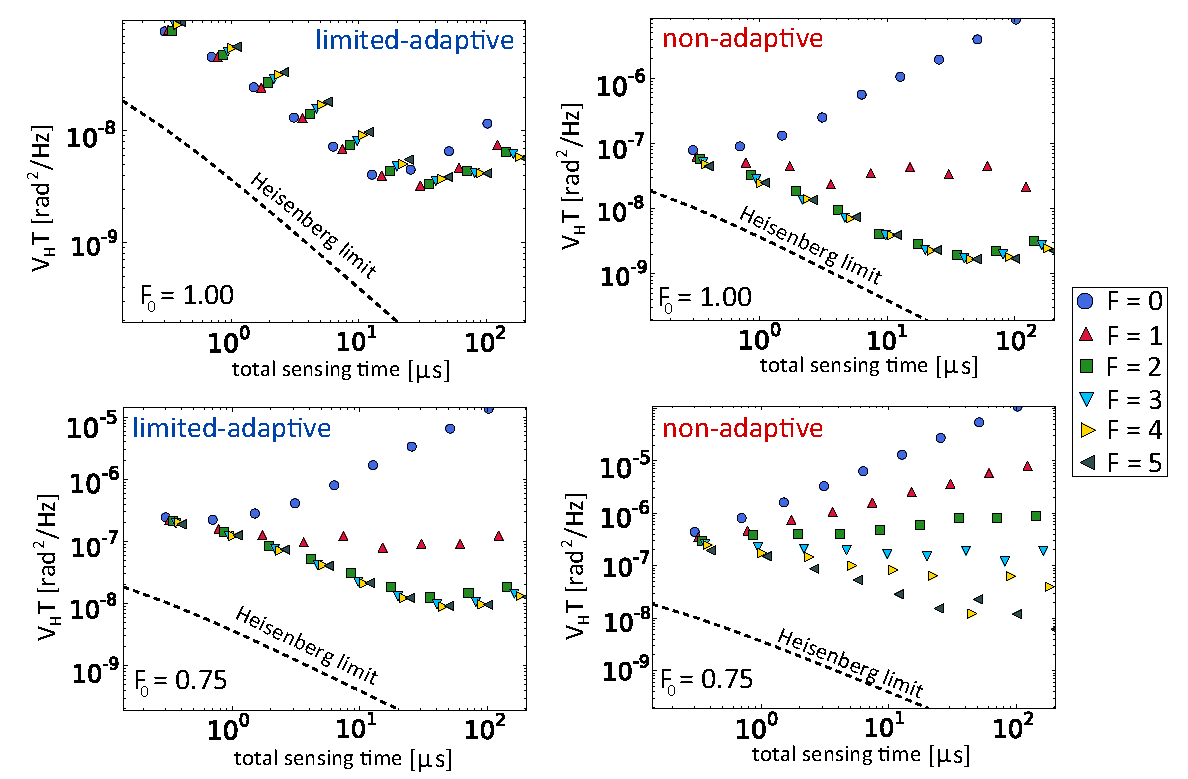
\includegraphics[width=12cm]{fig_S1}
	\caption{\label{fig:ammS1} \textbf{Non-adaptive vs limited-adaptive protocol}. Simulations comparing the limited-adaptive and non-adaptive protocols for $G = 5$, for different values of $F$, with $T_2^* = 5\mu$s. On the top row, perfect readout fidelity ($F_0 = 1$), on the bottom row, $F_0 = 0.75$. The shaded areas correspond to uncertainties (one standard deviation, calculated by a bootstrap technique). Note that the sensitivity is not further improved after the limit of $T_2^*$  is reached (total sensing time $T \sim 10\mu$s).
	}
\end{figure*}

\subsection{Limited-adaptive vs non-adaptive protocols.} 
The limited-adaptive protocol \cite{Cappellaro_Phys.Rev.A_2012} is described by the pseudo-code in Fig. \ref{fig:ammA1} (left). The controlled phase $\vartheta^{ctrl}$ is updated every time the sensing time is changed. 
In this section, the performance of the limited-adaptive protocol will be compared to the non-adaptive protocol described by Said et al. \cite{Said_Phys.Rev.B_2011} and demonstrated experimentally by Waldherr et al. \cite{Waldherr_NatNano_2012} and Nusran et al. \cite{Nusran_NatNano_2012}. The pseudo-code for the non-adaptive protocol is reported in Fig. \ref{fig:ammA1} (right). In this case, the phase of the Ramsey experiment is not updated in real-time based on the estimation of magnetic field given by the previous measurement outcomes, but its value is swept between 0 and $\pi$ according to predefined values. If, for a given sensing time, $M_n$ Ramsey experiments are performed, the Ramsey phase is increased at each step by $\pi$/$M_n$.


A comparison of the sensitivity as a function of sensing time \textit{T} for different values of \textit{F} (fixing \textit{G} = 5) is shown in \ref{fig:ammS1}. The data-points correspond to estimation sequences with increasing \textit{N} (\textit{N=} 2..10). The total sensing time \textit{T}, for each estimation sequence, is calculated as:

\begin{equation}
T=\tau_{min}[G(2^N -1)+ F(2^N - N - 1)]
\end{equation}

In top row of \ref{fig:ammS1} the sensitivities for the adaptive and non-adaptive protocols are compared in the case of perfect readout fidelities. In this case, the adaptive protocol follows a Heisenberg-like scaling already for \textit{F} = 0, even though the minimum sensitivity can only be reached for \textit{F} = 1. On the other hand, the non-adaptive protocol requires at least \textit{F} = 2 to reach Heisenberg-like scaling. On the bottom row, we compare the sensitivities for reduced readout fidelity ($F_0$ = 0.75). Here, the adaptive protocol reaches HL-scaling for $F\geq2$, while the non-adaptive protocol can only get close to it with $F=5$. 
It is important to stress that, in both cases, there is a big improvement when $M_n$ is a function of $n$ ($F>0$) compared to the case where $M_n$ is independent of $n$ ($F=0$). In other words, it is beneficial to repeat more often Ramsey experiments with shorter sensing time. The reason is two-fold: on one end they contribute less to the total sensing time, on the other end they are related to larger frequencies which, if estimated wrong, would give a larger error.

\begin{figure*}
	\centering
	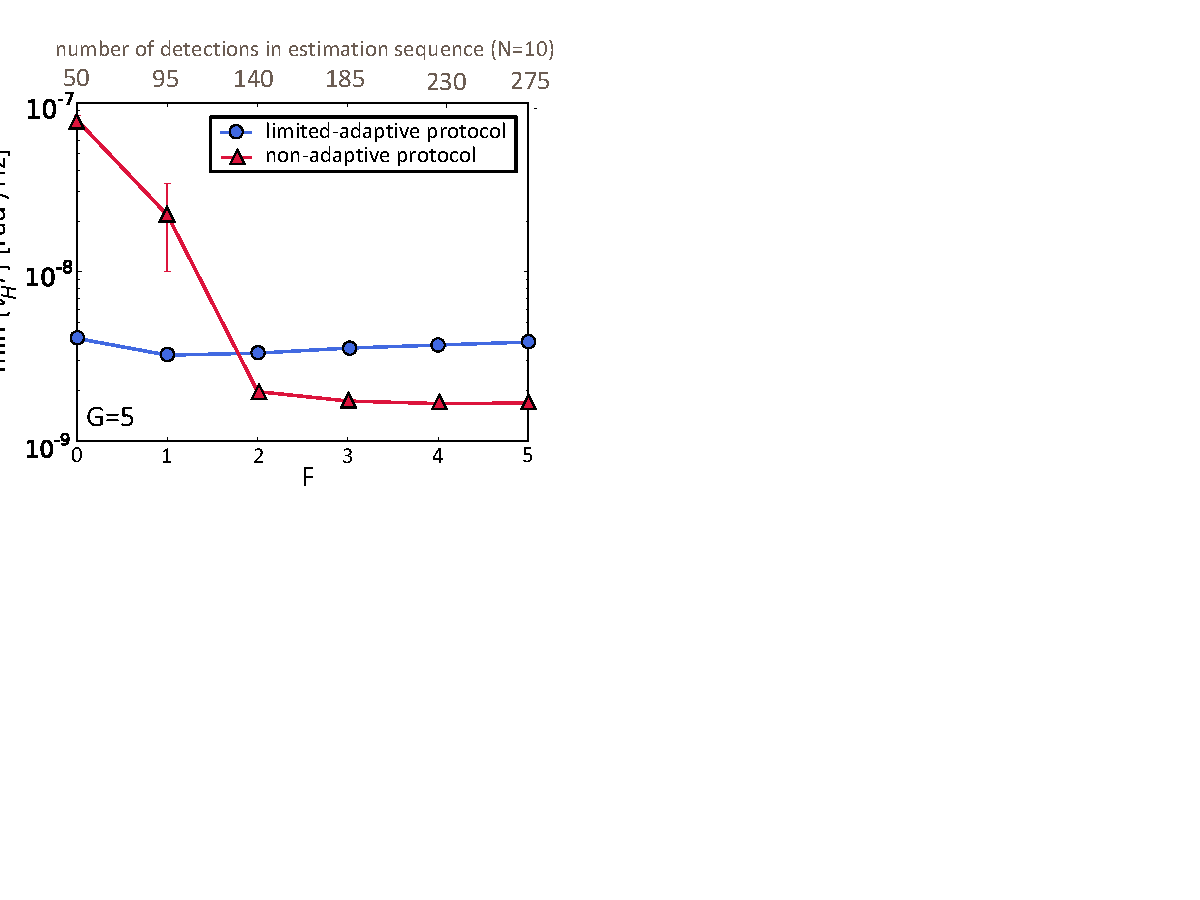
\includegraphics[width=6cm]{fig_S2}
	\caption{\label{fig:ammS2} \textbf{Simulation results for the best achieved sensitivity, comparing the limited-adaptive and non-adaptive protocols as a function of F}. Here, we assume perfect readout fidelity ($F_0=1$) and $T_2^* = 5\mu$s. On the top x-axis, the total number of Ramsey experiments in the estimation sequence for $N = 10$ is reported. Error bars, corresponding to one standard deviation, are calculated by bootstrap.
	}
\end{figure*}

Comparison between protocols is easier when plotting only the minimum sensitivity vs $F$. This is shown in Fig. \ref{fig:ammS2} for perfect readout fidelity $F_0=1$. We find that for $F<2$, the limited-adaptive protocol outperforms the non-adaptive protocol. This is expected since in this region only the limited-adaptive protocol exhibits Heisenberg-like scaling. However, once the non-adaptive protocol achieves Heisenberg-like scaling ($F\geq2$) it reaches a lower sensitivity.

On the scale at the top of Fig. \ref{fig:ammS2}, the number of Ramsey runs corresponding to an estimation sequence with $N = 10$ different sensing times is reported. By increasing $F$, the number of Ramsey experiments increases as:

\begin{equation}
R_N = GN + \frac{FN(N-1)}{2}
\end{equation}

For perfect readout fidelity, the limited-adaptive protocol reaches HL-scaling for $F=0$: therefore it only requires $R_N = 50$ Ramsey runs in the estimation sequence. On the other hand, the non-adaptive requires $F=2$, i.e. $R_N = 140$ Ramsey runs. Each Ramsey comprises an initialization/measurement duration, labelled as `overhead', not included in the plots (where we only take the sensing time into account). In practice, it is however necessary to minimize the total time of the sequence (including overhead), so that protocols that achieve Heisenberg-like-scaling with smaller $F$ (and therefore less detections $R_N$) are to be preferred as discussed in the main text (Fig. \ref{fig:amm-fig5}).


A striking result is the fact that once the non-adaptive protocol reaches Heisenberg-like-scaling it achieves a better sensitivity than the limited-adaptive one. Since non-adaptive protocols are a particular case of the most general class of adaptive protocols, this indicates that the limited-adaptive protocol is not optimal and that protocols with better performance must exist.

\subsection{Optimized adaptive protocol. }
\begin{figure*}[h!]
	\centering
	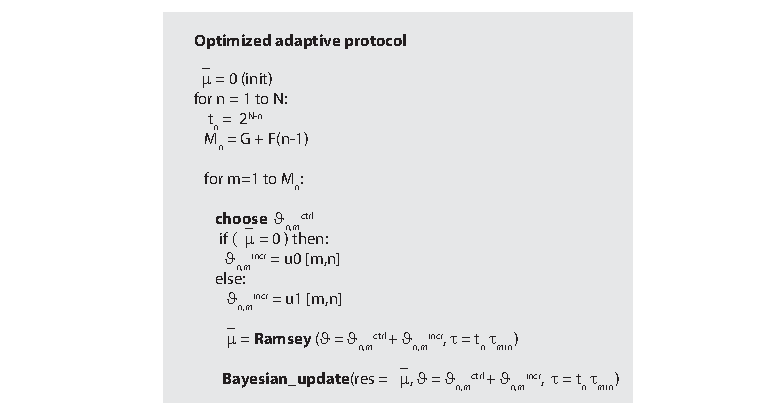
\includegraphics{algorithms_2}
	\caption{\label{fig:ammA2} \textbf{Pseudo-code for the optimized adaptive protocol.}}
\end{figure*}
In order to improve the performance of the limited-adaptive protocol, we consider two modifications:\\

Firstly, the controlled phase is estimated not only when changing sensing time, but before each Ramsey measurement (\textit{full-adaptive} protocol). The improvement achieved with this modification can be observed in Fig. \ref{fig:ammS3}, where we compare simulations for controlled phase updated only when changing sensing time and before each Ramsey. In the left plot, we compare the sensitivity, for increasing number of measurements $N$ ($N=2..10$) in the case ($G=3$,$F=0$). Both protocols scale better than the standard quantum limit only for the first few data-points (until $N>4$). However, the absolute sensitivity of the full-adaptive protocol is a factor two better. In the central plot, the same curves are displayed for ($G=3$,$F=5$). For these parameters, Heisenberg-like scaling is maintained until the coherence time limit is reached. Again, the full-adaptive protocol is better than the limited-adaptive for all $N$. In the right plot, we show the minimum achieved sensitivity for both protocols, as a function of $F$. In all cases the full-adaptive protocol outperforms the protocol which updates the optimal phase only when changing the sensing time. Additional simulations (not shown) for different values of $G$, or imperfect readout fidelity, confirm the improvements gained by the full-adaptive strategy. \\
\begin{figure*}
	\centering
	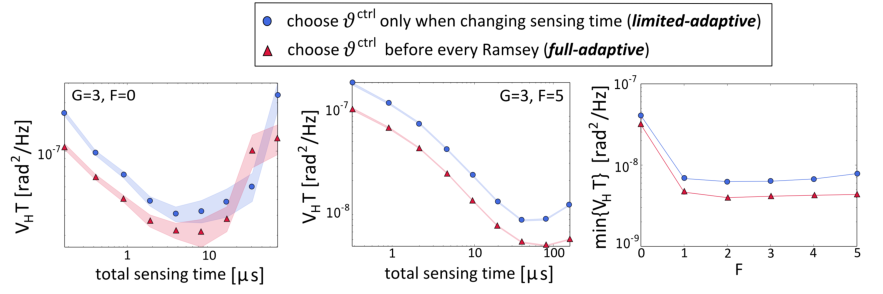
\includegraphics[width=12cm]{fig_S3_new}
	\caption{\label{fig:ammS3} \textbf{Comparison adaptive protocols} Adaptive protocols: simulation results comparing sensitivities obtained when updating the controlled phase only when changing sensing time (blue) and updating it before each Ramsey (red). We assume perfect readout fidelity and $T_2^* = 5\mu$s. Shaded areas represent error bars corresponding to one standard deviation (bootstrap method). 
	}
\end{figure*}
The second modification was suggested by A. J. Hayes and D. W. Berry \cite{Hayes_Phys.Rev.A_2014}. They proposed a protocol where the detection phase of the Ramsey experiment is $\vartheta_{(n,m)} = \vartheta_{(n,m)}^{ctrl} + \vartheta_{(n,m)}^{incr}$. A phase increment $\vartheta_{(n,m)}^{incr}$, dependent only on the last measurement outcome, is added to the controlled phase $\vartheta_{(n,m)}^{ctrl}$. The phase increment is obtained by numerically optimizing the final variance in frequency estimation for the specific experimental parameters through a \textit{swarm optimization} procedure\cite{Hayes_Phys.Rev.A_2014,Hentschel_Phys.Rev.Lett._2010,Bratton__2007}. In the pseudo-code this step is represented by the functions u0, u1. \\

The optimized adaptive protocol, described in Fig. \ref{fig:ammA2}, combines phase increments with update of the controlled phase before each Ramsey. A comparison between the minimum sensitivity achieved by the limited-adaptive, non-adaptive and optimized-adaptive protocols is reported in Fig. \ref{fig:ammS4}. The optimized adaptive protocol appears to perform always at least as good as the best between the limited-adaptive and the non-adaptive protocols. For lower values of $F$, the non-adaptive protocol fails to reach HL-scaling, while both adaptive ones do. For higher values of $F$, both the non-adaptive and the optimized adaptive reach the minimum sensitivity. Note that, for a readout fidelity $F_0 = 0.88$, while the optimized adaptive protocol reaches HL-scaling for ($G = 5$,$F = 2$) the non-adaptive one needs at least $F = 4$.


\begin{figure*}
	\centering
	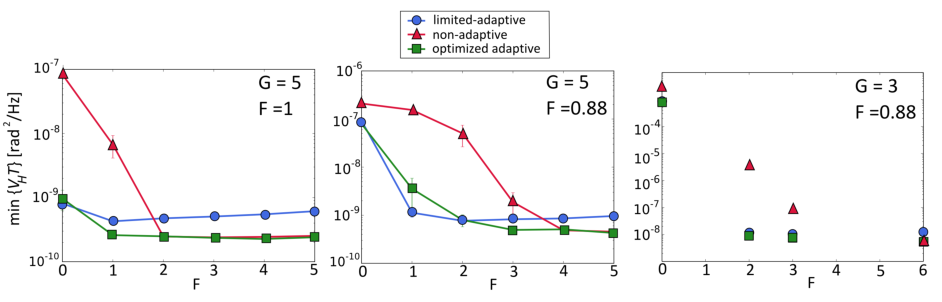
\includegraphics[width=12cm]{fig_S4_new}
	\caption{\label{fig:ammS4} \textbf{Comparing all protocols.} Simulations comparing the best achieved phase sensitivities for different protocols ($G = 5$ left and central plots, $G = 3$ for the plot on the right). We assume $T_2^* = 96\mu$s. The optimized adaptive protocol performs always at least as well as the non-adaptive protocol. For a fixed value of $G$, the optimized adaptive protocol reaches the best sensitivity for a smaller value of $F$.
	}
\end{figure*}
\section{Application to room-temperature sensing.}
\label{sec:ammSIRTsens}
\begin{figure*}
	\centering
	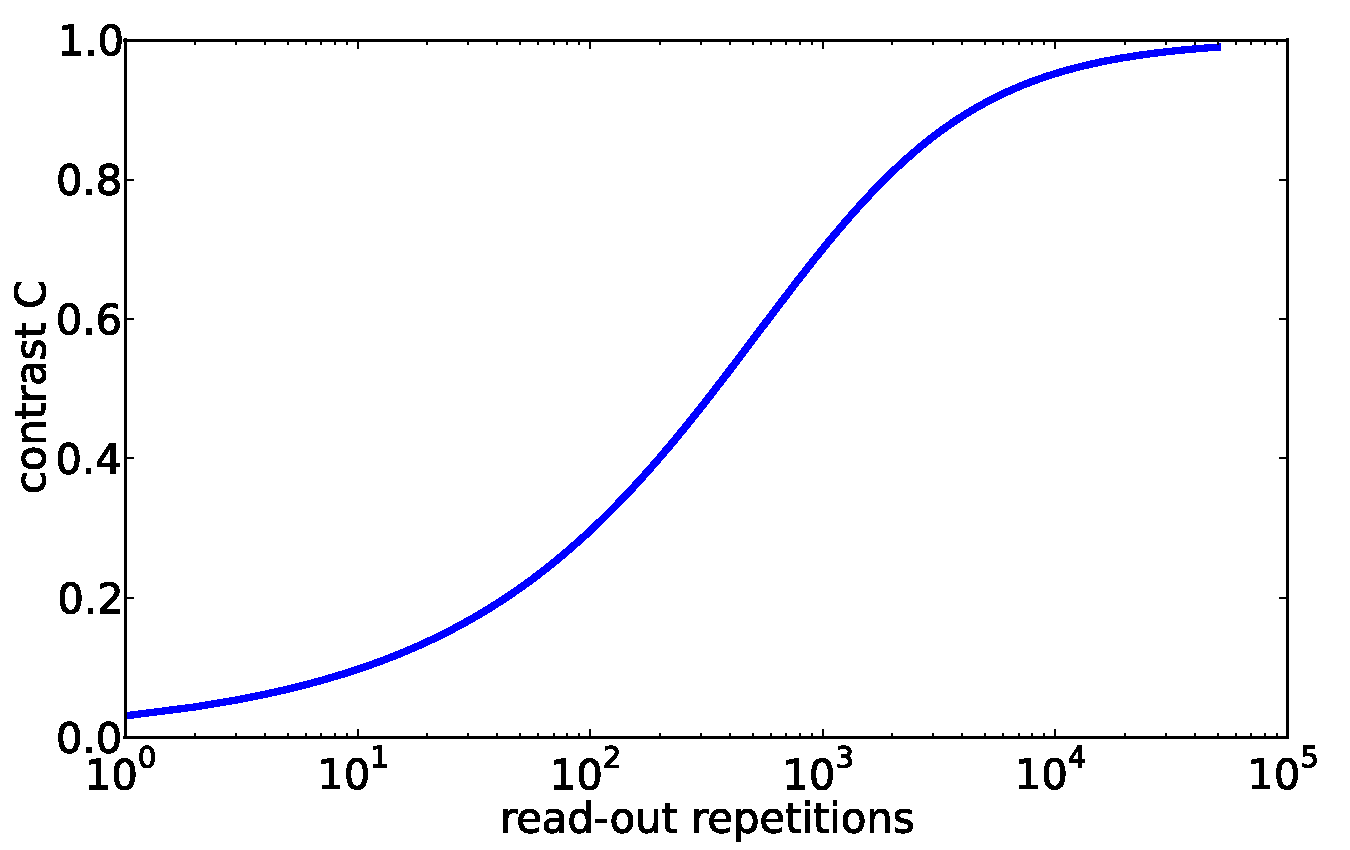
\includegraphics[width=6cm]{fig_S5}
	\caption{\label{fig:ammS5} \textbf{Contrast for room-temperature readout} Effective readout fidelity as a function of readout repetitions, for measurements at room-temperature (no single-shot readout).
	}
\end{figure*}

At room-temperature, the spin-selective optical transitions within the zero-phonon line are not spectrally-resolvable and therefore single-shot spin initialization and readout by resonant optical excitation is not possible. Instead, the readout exploits the small difference in luminescence intensity by off-resonant optical excitation (in the green) when the electron spin is in $m_s = 0$, compared to $m_s = 1$. In the following, we will use numbers from Nusran et al. \cite{Nusran_NatNano_2012}, that report $\alpha_0 = 0.031$ photons per shot when the electron is in $m_s = 0$, $\alpha_1 = 0.021$ photons per shot when the electron is in $m_s = 1$.  Since one shot is not enough to perfectly distinguish between the two states, room-temperature experiments are repeated $R$ times. The resulting signal level is then, respectively, $\alpha_0 R$ and $\alpha_1 R$. The contrast $C$ for a single repetition scales as \cite{Taylor_NatPhys_2008}:

\begin{equation}
\frac{1}{C} = \sqrt{1+\frac{2(\alpha_0 + \alpha_1)}{(\alpha_0-\alpha_1)^2R}}
\end{equation}

\begin{figure*}
	\centering
	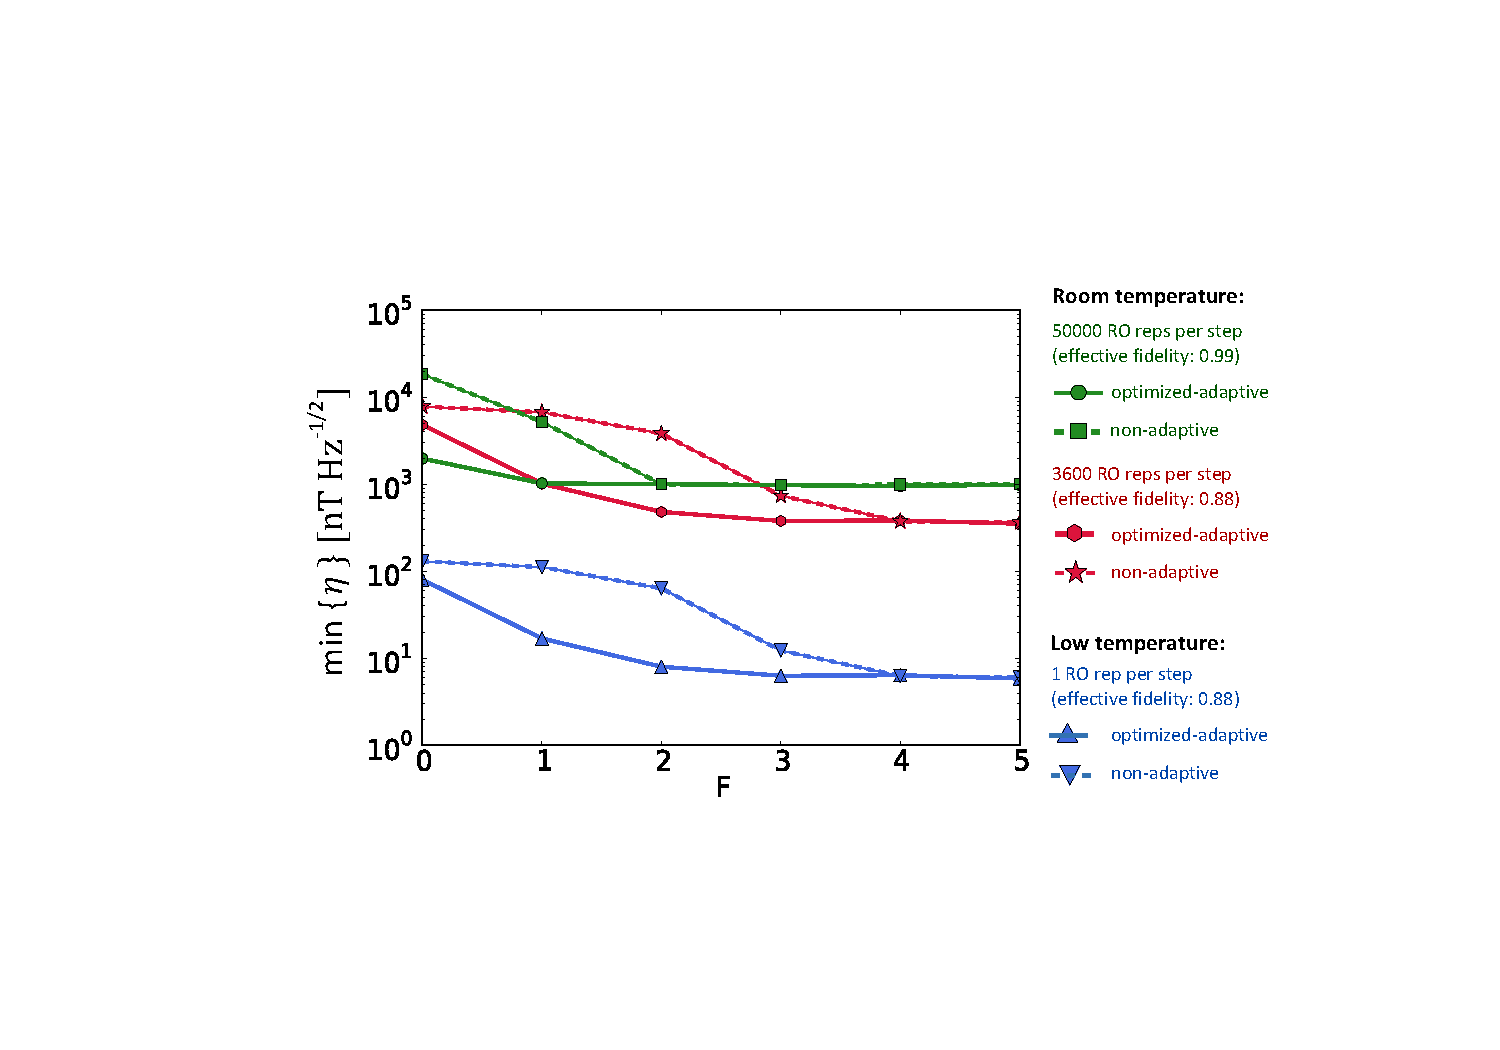
\includegraphics[width=12cm]{fig_S6}
	\caption{\label{fig:ammS6} \textbf{Adaptive protocol for room-temperature} Simulations comparing the minimum magnetic field sensitivity (in nT Hz$^{-\frac{1}{2}}$) for the optimized adaptive and the non-adaptive protocols at room-temperature and low-temperature ($T_2^* = 96 \mu$s, $N = 10$, $G = 5$). 
	}
\end{figure*}
This contrast $C$ is related to the fidelity with which the two states can be distinguished and, since luminescence detection is shot-noise limited, the error scales at the standard quantum limit as $R^{-\frac{1}{2}}$. Nusran et al. achieve a fidelity of 0.99, in their experiment \cite{Nusran_NatNano_2012}, by using 50000 readout repetitions per step. The achieved contrast as a function of readout repetitions is plotted in Fig \ref{fig:ammS5}.
A contrast $C = 0.75$ can be achieved with $R = 1350$ repetitions, while $R = 3600$ repetitions are needed for $C = 0.88$, significantly less than the repetitions (50000) needed for almost perfect readout ($C = 0.99$). 
In the simulations in Fig. \ref{fig:ammS6}, for consistency with previous results, we assume asymmetric readout fidelity ($F_1 = 0.993$,$F_0 = C+(1-F_1)$), based on the contrast $C$ achieved with a given number of readout repetitions. The asymmetry of the readout fidelity can be controlled at will by choosing the threshold in photo-counts distinguishing $m_s = 0$ from $m_s = 1$.

Simulation results show that, at room temperature, the use of 50000 repetitions can achieve a sensitivity of $\eta \sim 1$ $\mu$T Hz$^{-\frac{1}{2}}$, either using the adaptive or non-adaptive protocols. However, using 3600 repetitions per step (with a lower effective readout fidelity), a better sensitivity $\eta \sim 0.4$ $\mu$T Hz$^{-\frac{1}{2}}$ can be reached. Moreover, for $F = 2$, the performance of the optimized-adaptive protocol with 3600 readout repetitions per step surpasses both the performance of the non-adaptive for the same conditions and the performance of the protocols with 50000 repetitions per step. For $F \geq 4$ adaptive and non-adaptive reach the same sensitivity: however, as discussed above and in the main text, a smaller value of $F$ allows a higher repetition rate of the estimation sequence.

This suggests the possibility that adaptive sensing, which reaches Heisenberg-limited scaling for a reduced number of measurements even in situation of lower fidelity, may be advantageous for room-temperature sensing, compared to non-adaptive protocols.
Simulations confirm the superior performance of the protocol in the case where single-shot readout is available, enabling sensitivities on the order of a few nT Hz$^{-\frac{1}{2}}$, as demonstrated experimentally by the data reported in the main text.


\section{Experimental techniques}

Microwave (MW) signals to drive the NV centre electron spin are generated by a Rohde Schwarz SMB100A source, with IQ modulation.  To create the two $\pi$/2 pulses for each Ramsey experiment, the MW source output frequency is modulated (single-sideband modulation) by two pulses with rectangular envelope and 30 MHz carrier frequency. The first pulse is generated directly by an AWG (Arbitrary Waveform Generator, Tektronix AWG5014), the second by a field-programmable logic array (FPGA). The FPGA receives the value for the phase $\vartheta$ chosen by the control microprocessor (ADwin Gold) and generates the modulation pulse with the proper IQ parameters, with timing triggered by the AWG. The value for the phase $\vartheta$ is specified as an 8-bit integer (256 levels), leading to a resolution of 1.4 degrees (0.025 radians).
Due to the hyperfine coupling to the host $^{14}$N spin, the electron spin transition is split into three frequency-separated lines. As discussed in Section \ref{sec:ammMW}, these three lines are addressed separately by three Ramsey experiments, realized by driving the electron spin at the three frequencies. This is achieved by an additional frequency modulation, imposed to the vector source by the AWG. The microprocessor (Adwin Gold) manages the sequence  of control pulses (optical and microwave) and counts the luminescence photons during spin readout. Moreover, it performs the Bayesian update of the probability density distribution $P(f_B)$ and chooses the proper controlled phase and phase increments. 

\subsection{Bayesian estimation with microprocessor}
\label{ammSI:overhead}
The microprocessor code for Bayesian update minimizes the number of coefficients $p_k$ (Eq. S-E2) to be tracked and stored, to avoid exceeding the memory bounds of the microprocessor, and to optimize speed. We only use the coefficients which are known to be non-zero and contribute to the choice of the controlled phase $\vartheta$, neglecting the rest. Since the probability distribution is real ($p_k^* = p_{-k}$), we can further reduce the computational requirements by only storing the coefficients for $k>0$. Considering all this, the number of coefficients that needs to be processed, at each step $n$, is on the order of $M = G+F(n-1)$.

\begin{table}[]
\centering
\begin{tabular}{ccccc}
\hline
\multicolumn{1}{l}{\textbf{N}} & \multicolumn{1}{l}{\textbf{\begin{tabular}[c]{@{}l@{}}initialization\\ time {[}ms{]}\end{tabular}}} & \multicolumn{1}{l}{\textbf{\begin{tabular}[c]{@{}l@{}}sensing\\ time {[}ms{]}\end{tabular}}} & \multicolumn{1}{l}{\textbf{\begin{tabular}[c]{@{}l@{}}readout\\ time {[}ms{]}\end{tabular}}} & \multicolumn{1}{l}{\textbf{\begin{tabular}[c]{@{}l@{}}computational\\ time {[}ms{]}\end{tabular}}} \\ \hline
\rowcolor[HTML]{C0C0C0} 
\textbf{5}  & 9.0 & 0.004 & 1.80 & 4.0 \\
\textbf{7}  & 15.4 & 0.018 & 3.08  & 8.0  \\
\rowcolor[HTML]{C0C0C0} 
\textbf{8}  & 19.2 & 0.035 & 3.84 & 10.8  \\
\textbf{9}  & 23.4 & 0.071 & 4.68 & 13.9 \\
\rowcolor[HTML]{C0C0C0} 
\textbf{10} & 28.0 & 0.140 & 5.60  & 17.6 \\
\textbf{12} & 38.4 & 0.573 & 7.68  & 26.8  \\ \hline
\end{tabular}
\caption{\textbf{Temporal budget of the estimation protocol.} Total time, measured by the internal microprocessor clock, spent by the optimized-adaptive protocol in different tasks within the whole estimation sequence. The computational time (i.e. the time spent by the processor in performing the Bayesian update), is similar to that spent on spin initialization. Given that initialization and Bayesian update can be performed simultaneously, the computational time represents no additional overhead. }
\label{tab:ammtable_overhead}
\end{table}
In the case ($G = 5$, $F = 2$), the time spent by the microprocessor in the Bayesian update after each Ramsey experiment increases linearly from 80 $\mu$s (for $n = 2$) to 190 $\mu$s (for $n = 12$). This time is comparable with the spin initialization duration (200 $\mu$s). In Table \ref{tab:ammtable_overhead} we show the total times associated with sensing, initialization, and computation of the Bayesian estimate. While in this work we performed the initialization and the Bayesian estimate sequentially, both operations can be performed simultaneously. In this way the real-time Bayesian estimation, a crucial prerequisite for the adaptive technique, does not add any temporal overhead to the protocol. In future implementations, the Bayesian estimation could be implemented with a dedicated FPGA, instead of a general-purpose microprocessor, which would allow a further reduction of the calculation time.

\subsection{Microwave pulses and coupling to the $^{14}$N spin}
\label{sec:ammMW}
When using the electron spin of the NV center as a sensor in a Ramsey interferometry experiment, the coupling to its host $^{14}$N nuclear spin has to be taken into account. The hyperfine interaction ($\hat{H}_{hf}=A_{hf} \hat{S}_z \hat{I}_z$, neglecting small off-diagonal terms) effectively splits the electron spin $m_s = 0 $ to $m_s = -1$ transition in three lines (Fig. \ref{fig:ammS7}b).  Although these three lines can be addressed simultaneously by selecting a Rabi frequency larger than the coupling strength, the phase acquired during free evolution will depend on the state of the $^{14}$N spin. This creates ambiguity in the frequency estimation protocol, since the aim is to sense only the change in energy levels introduced by the Zeeman shift induced by the applied magnetic field, not the coupling to the $^{14}$N spin.

To circumvent this problem, we perform three sequential Ramsey sequences where, in each sequence, the microwave pulses are resonant with one of the three $m_s = 0$ to $m_s = -1$ transitions and the acquired phase only depends on the Zeeman shift. We choose the Rabi frequency (140 kHz) such that the pulses in each sequence only address selectively one of the three transitions. In Fig. \ref{fig:ammS7}, we show that we can perform Rabi oscillations selectively on the Nitrogen spin. Here the microwave pulses only drive the electron spin $m_s = 0$ to $m_s = -1$ transition if they are on resonance, thus for the $^{14}$N spin in a mixed state, a contrast of 1/3 is expected. Full contrast is recovered when the three pulses are applied sequentially (Fig. \ref{fig:ammS7}c).

\begin{figure*}
	\centering
	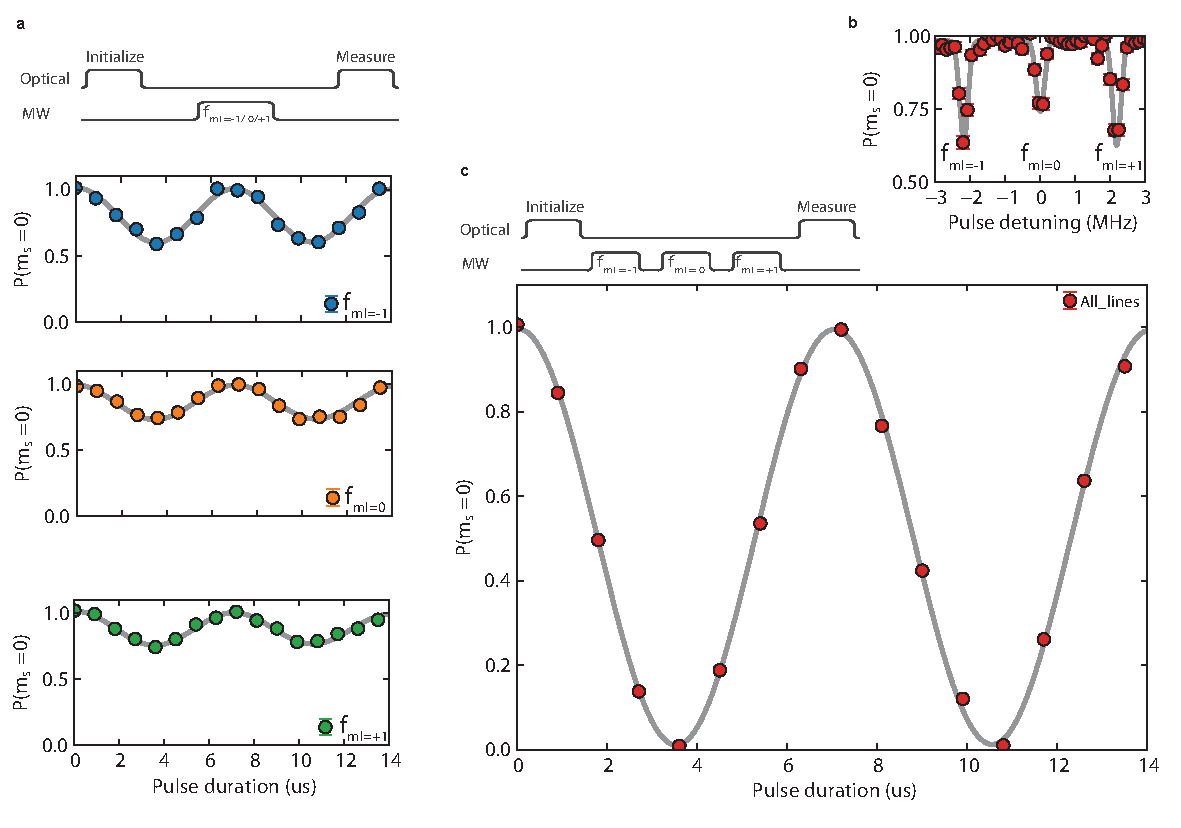
\includegraphics[width=12cm]{Rabi_diff_hf_lines}
	\caption{\label{fig:ammS7} \textbf{Electron spin driving.} a) Rabi oscillations of the electron spin conditional on the state of the  nitrogen spin ($^{14}$N , $I = 1$). We tune the frequency of the microwave pulses in resonance with one of the three $m_s = 0$ to $m_s = -1$ transitions, corresponding to the nitrogen spin being either in $m_I = -1 , 0$ or $+1$ (top, middle bottom) and vary the length of the pulse. From a sinusoidal fit (grey line) we find Rabi frequencies of  (144, 140 and 142 $\pm$ 2 kHz) respectively b) Energy level spectrum for the electron $m_s = 0$ to $m_s = -1$ transition. We initialize the electron spin in $m_s = 0$ and then vary the frequency of a microwave pulse with fixed length. The pulse detuning is with respect to a reference frequency of 2.845334 GHz.  The spectrum shows three lines owing to the hyperfine interaction with the $^{14}$N spin with $|A_{hf}| = 2\pi x (2.185  \pm 0.006)$ MHz. c) Rabi oscillation of the electron spin unconditional on the state of the nitrogen spin. We apply three sequential microwave pulses each on resonance with one of the hyperfine lines. From the sinusoidal fit (grey line) we find a Rabi frequency of $(142 \pm 3)$ kHz.}
\end{figure*}

We note that this method requires the electron transition energies and therefore the static magnetic field to be known within the bandwidth of the pulses ($\sim$ 140 kHz). This is not a problem for our implementation, where the effect of an external field is implemented as an artificial detuning by adjusting the phase of the final $\pi$/2 pulse. When estimating a real magnetic field possible solutions would be to initialize the nitrogen spin, adjust the frequency estimation protocol to allow for sensing of multiple frequencies with fixed offset or adjust the interaction times such that the phase acquired during free evolution is independent of the state of the nitrogen spin ($2 \pi = \tau A_{hf}$).

\subsection{NV charge state and optical resonance pre- and post-selection.}
Due to environmental charge noise, the optical transitions of the NV centre shift in frequency on a range larger than the linewidth. Moreover, resonant excitation can result in ionization of the NV$^-$ charged state into the neutral NV$^0$ state.
Before each estimation sequence, we check that the centre is in the NV$^-$ state, with optical transitions resonant with the excitation lasers. We turn both the initialization and readout lasers (on transitions E’ and $E_y$, respectively) for 150 $\mu$s and count luminescence photons. Only if the luminescence photo-counts are larger than a given threshold (40 counts), the estimation sequence is started (charge and optical resonance pre-selection). We take the absence of luminescence photo-counts as an indication that the centre is ionized into the NV$^0$ state: the correct charge state is restored by resonant optical excitation of the NV$^0$ transition at 575 nm.
An estimation sequence can consists of a large series of Ramsey experiments, with spin initialization and readout. Ionization of the defect or large frequency shifts of the optical transitions during the sequence results in incorrect spin readout and errors in the magnetic field estimation. Therefore, we perform a new check of the charge and optical resonance conditions at the end of the estimation sequence and consider it as a valid estimation only if more than 10 luminescence photo-counts are detected (charge and optical resonance post-selection).
In the histograms in Fig. \ref{fig:ammS8}, we report an example of the number of rejected runs for 225 repetitions of the estimation sequence. While the average number of rejections in the post-selection process is around 50\%, we have a consistent fraction of events (75/252) with no rejections, and other runs with 80\% failure rate. This large spread is due to the fact that the data was taken in long automated measurement session during nights, with infrequent optimizations of the experimental parameters (like spatial overlap of laser beams on the NV centre). We believe that the percentage of rejected runs can be drastically reduced by optimizing the experimental settings and procedures.
\begin{figure*}
	\centering
	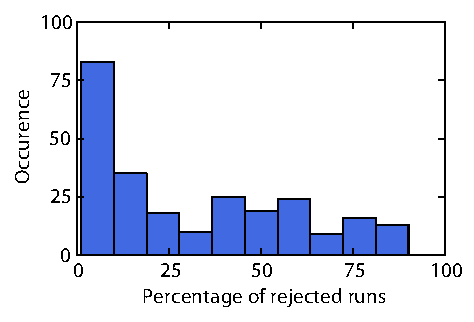
\includegraphics{Failed_CR_checks}
	\caption{\label{fig:ammS8} \textbf{Charge resonance statistics.} Histograms of the percentage of rejected runs in charge and optical resonance post-selection.}
\end{figure*}
\bibliographystyle{../thesis}
\bibliography{amm_appendix}

\graphicspath{{./ch_adptv_msmnt_cntrl_SI/figures/}}


\chapter{Implementation of partial measurements}
\label{ch:AMCappendix}

\def\bra#1{\left<#1\right|}
\def\ket#1{\left|#1\right>}
\def\dm#1{\left|#1\right> \left<#1\right|}


\section*{Levels and Hamiltonian}
The NV center forms a natural two qubit system: the electron spin serves as the ancilla qubit, while the system qubit is implemented on the spin of the NV nitrogen atom. The relevant levels are plotted in Fig. \ref{fig:levels}: the full level scheme can be found in the Supporting Online Material of Pfaff \textit{et al}. \cite{Pfaff_NatPhys_2012}.\\
The electron spin is given by the collective spin of the the six unpaired electrons of the negatively-charged state of the center, which constitute a spin $S=1$ system. The $m_s=0$ state is separated from the $m_s=\pm1$ states by the zero-field splitting ($D = 2.878 \pm 0.001$ GHz). The $m_s=-1$ and $m_s=+1$ states are split by $ 98$ MHz by an external magnetic field ($B = 17.5 G$). The ancilla qubit is defined by the $m_s=0  (\ket{0})$ and $m_s=-1  (\ket{1})$ states. Electron spin rotations are performed by microwave pulses, with a Rabi frequency of $ 7.67$ MHz. The probability to excite the $m_s=+1$ spin state when driving microwaves is negligible. The electron spin coherence time has been measured to be $T_2^* = (1.35 \pm 0.03)$ $\mu$s by a Ramsey experiment.\\
The NV's nitrogen atom ($^{14}N$) carries $I=1$ spin and the system qubit is defined by the $m_I = -1 (\ket{\Uparrow})$ and $m_I=0 (\ket{\Downarrow})$ levels, separated in frequency by $\Omega_N = |Q| + g_N \mu_N B \sim 2 \pi \times 5$ MHz, where $Q$ is the nuclear quadrupole splitting $Q = -2\pi \times 4.98 $ MHz. The hyperfine interaction between the electron and nuclear spin has the form $\mathcal{\hat{H}}_{hf} \sim A_z \hat{I}_z \hat{S}_z$ (neglecting small off$-$diagonal terms), which further splits the nuclear levels by an amount $A_z = -2\pi \times 2.184 \pm 0.002$ MHz when the electron is in the $m_s=-1$ manifold.
Nuclear spin rotations are performed by radio-frequency pulses, with a Rabi frequency of $17$ kHz. The nuclear spin coherence time has been measured by a Ramsey experiment to be $T_2^* = 7.8 \pm 0.3$ ms (Fig. \ref{fig:nuclearSpin}).\\

\begin{figure} [h]
\centering
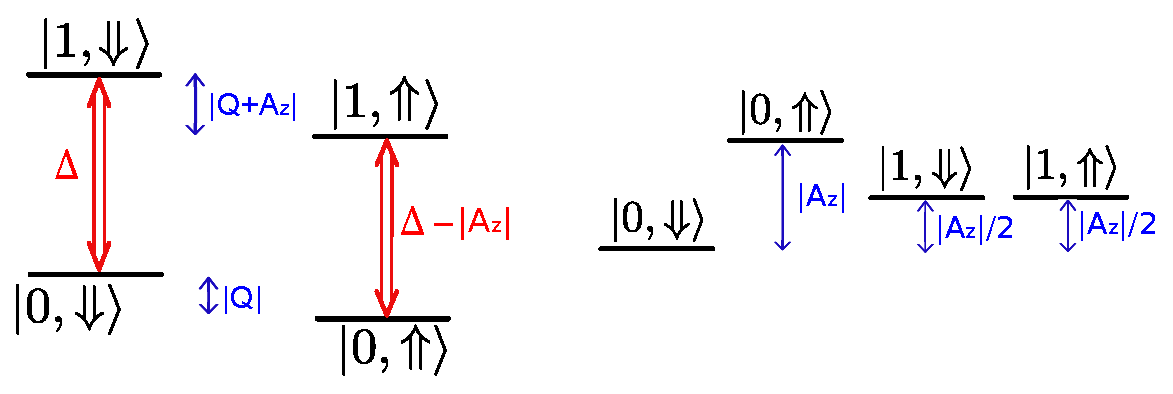
\includegraphics [width = 12 cm]{SOM/fig01_levelScheme.eps}
\caption{\textit{ On the left, scheme of the relevant energy levels for the electron and nuclear spin qubits. On the right, level energies in a doubly-rotating reference frame, rotating at frequency $\omega_e = \Delta-|A_z|/2$ for the electron spin, and $\omega_n = |Q+A_z|$ for the nuclear spin.}}
\label{fig:levels}
\end{figure} 


The Hamiltonian of the system is $\mathcal{\hat{H}}=\mathcal{\hat{H}}_0 +\mathcal{\hat{H}}_{drive}$, with:
\begin{equation}
 \mathcal{\hat{H}}_0 = -|Q| \dm{0, \Uparrow} + \Delta \dm{1, \Downarrow}+(\Delta-|Q+A_z|)\dm{1, \Uparrow}
\end{equation}
and:
\begin{equation}
 \mathcal{\hat{H}}_{drive} = \Omega_{MW} (t)  \hat{S}_{x} \otimes \mathbb{\hat{1}}_N  + \Omega_{RF} (t) \ket{1}\bra{1} \otimes \hat{I}_x + \mbox{h. c.}
 \label{Eq:ham0}
\end{equation}
where $\Delta= D -g_e \mu_eB = 2.8288 \pm 0.0002$  GHz and $\hat{S}_i$, $\hat{I}_i$ are respectively the Pauli operators for the electron spin and the nuclear spin. \\

The Hamiltonian in Eq. \ref{Eq:ham0} is time-dependent and state evolution has, in general, no analytical solution. In order to simplify the problem, we apply the rotating-wave approximation \cite{Slichter__1996}, using a doubly-rotating frame: one rotating at the driving frequency for the electron spin, and the other one at the driving frequency for the nuclear spin. We set the microwave  frequency ($\omega_e = \Delta-|A_z|/2$) such that it is detuned by $|A_z|/2$ from both hyperfine transitions and the RF-field is on resonance with the nuclear spin transition in the $m_s=-1$ electron spin manifold ($\omega_N = |Q+A_z|$). Applying the unitary transformation $\hat{U} = e^{-i \left( \omega_N \mathbb{\hat{1}}_e \times \hat{I}_z + \omega_e \hat{S}_z \times \mathbb{\hat{1}}_N \right) t}$ and retaining the secular terms, the Hamiltonian, in the basis $\{ \ket{0, \Downarrow}, \ket{0, \Uparrow}, \ket{1, \Downarrow}, \ket{1, \Uparrow}  \}$, becomes:

\begin{equation}
\mathcal{\hat{H}'} = \left[
\begin{array}{cccc}
0 & 0 & \Omega^*_{MW} & 0\\
0 & |A_z| & 0 & \Omega^*_{MW}\\
\Omega_{MW} & 0 & |A_z|/2 & \Omega^*_{RF}\\
0 & \Omega_{MW} & \Omega_{RF} & |A_z|/2
\end{array}
\right]
\label{eq:H0_RWA}
\end{equation}

The energy levels, in the rotating-wave approximation, are shown on the right side of Fig. \ref{fig:levels}. We define the positive quantity $A$ to be $A = |A_z|$ in the rest of the Supplementary Information.

\section*{Qubit initialization}
\label{sec:qubitinit}
The electron spin is initialized in the $m_s=0$ state by optical spin-pumping with a fidelity $0.983 \pm 0.006$ \cite{Robledo_Nature_2011}. We use the forbidden transition of $E_{y}$ which is detuned by $\Delta$ from the spin-preserving $E_{y}$-transition. This transition is well suited for a reset of the electron spin during the protocol, since flip-flops with the nuclear spin are suppressed due to selection rules. \\

\begin{figure} [h]
\centering
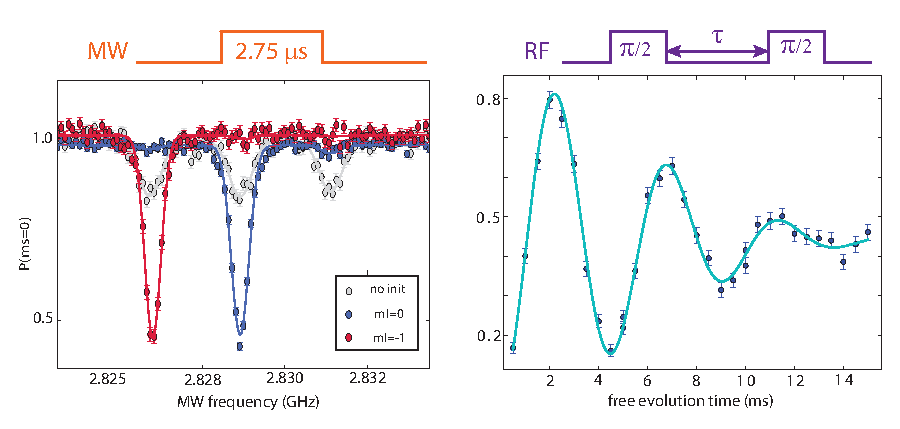
\includegraphics [width = 12 cm]{SOM/fig02_nuclearSpin_v2.eps}
\caption{\textit{On the left, nuclear spin initialization. The nuclear spin is initially unpolarized (gray): the ESR spectrum for the $m_s=-1 \leftrightarrow 0$ transition shows three hyperfine lines, corresponding to $m_I=-1,0,+1$. By measurement-based initialization (MBI) \cite{Pfaff_NatPhys_2012} we can initialize the spin in any of the nuclear spin states (blue/red). On the right, nuclear spin Ramsey. The nuclear spin is initialized by MBI after which the free evolution time $\tau$ between two $\pi/2$-pulses is varied. The solid line is a fit to the function $y_0 + e^{-(\frac{\tau}{T_{2}^{*}})^2}\cos{(\omega_{det} \tau + \phi )}$ from which we find the dephasing time $T_2^* = 7.8 \pm 0.2$ ms.}}
\label{fig:nuclearSpin}
\end{figure} 

The nuclear spin is initialized by measurement \cite{Pfaff_NatPhys_2012} as shown in Fig. \ref{fig:nuclearSpin}. We prepare the electron spin state in $\left| m_s=\pm 1 \right \rangle$ by spin-pumping on the $E_{y}$ transition. We apply a selective microwave $\pi$-pulse ($f_{rabi} = 181.8$ kHz) to the electron, on resonance with one of the three hyperfine lines. We then read-out the electron spin state, by exciting the $E_y$ transition. In case of photon detection, the electron state is projected to $m_s=0$, and the nuclear spin is projected on the state that was addressed by the microwave pulse.
During the selective microwave pulse, the electron spin undergoes significant dephasing, reducing the success probability, but not the initialization fidelity of the nuclear spin. The measured initialization fidelity is $0.95 \pm 0.02$, obtained from the fitting the heigth of the peaks in Fig. \ref{fig:nuclearSpin}  and the success probability is around $0.07$. The success probability is determined by $p = p_{m_s=-1} \cdot p_{m_I=-1} \cdot p_{e-flip} \cdot p_{phot}$, where the relevant parameters are:
\begin{itemize}
 \item $p_{m_s=-1} \sim 0.5$ is the probability to spin pump the electron spin in $m_s=-1$ (in the remaining cases it's in $m_s = +1$).
 \item $p_{m_I=-1} \sim 1/3$ is the population of the desired state $m_I=-1$ for an initially unpolarized nuclear spin.
 \item $p_{e-flip} \sim 0.6$ is the success probability of nuclear-dependent electron spin rotations.
 \item $ p_{phot} \sim 0.6-0.8$ is the probability to detect a photon when reading-out the $m_s=0$ state, limited by the collection of the optical system and the finite photon detection efficiency.
\end{itemize}


\section* {Nucleus-independent electron spin rotations}
\label{sec:uncond_rot_MW}
The maximum Rabi frequency we achieve in the setup is $\sim 8$ MHz (Fig. \ref{fig:rabi}). Given the hyperfine splitting of 2.184 MHz, these pulses introduce off-resonant driving errors that limit the weakest measurement we could achieve to $\theta = 15$ degrees ($C = 0.27$, see equation \ref{eq:concurrence}). To overcome this problem, we use CORPSE pulses \cite{Cummins_PRA_2003}, a composite pulse sequence designed to compensate for off-resonance errors. The weakest measurement we achieve with the CORPSE pulses is $\theta_{min} = 5$ degrees, corresponding to $\tau = 12$ ns (obtained from a fit of the Ramsey fringes in Fig. \ref{fig:amc-fig1}b of the main text)

\begin{figure} 
\centering
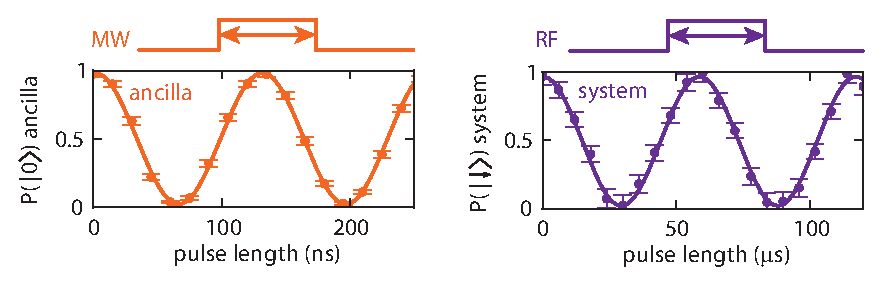
\includegraphics [width = 12 cm]{SOM/rabi.eps}
\caption{\textit{Coherent single-qubit rotations of the electron spin ancilla qubit (orange) and the nuclear spin system qubit (purple) are performed by varying the length of a MW (RF) pulse. Solid lines are sinusoidal fits from which we determine the Rabi frequency  $7.67 \pm 0.02$ MHz / $17.07 \pm 0.01$ kHz).}}
\label{fig:rabi}
\end{figure} 

\section*{Electron-independent nuclear spin rotation}
\label{sec:uncond_rot_RF}
For quantum state tomography and for weak-value measurements, we need to be able to perform nuclear spin rotations, unconditional on the electron spin state. This is not trivial if the electron and nuclear spins are entangled.
In particular, when the electron is in the $\left| m_s=-1 \right \rangle$ state, the splitting between $\left| \Downarrow \right \rangle$ and $\left| \Uparrow \right \rangle$ is $\omega_N^{(-1)} = |Q+A_z| = 2\pi \times 7.164$ MHz, while when the electron in the $\left| m_s=0 \right \rangle$ state, $\omega_N^{(0)} = |Q| = 2\pi \times 4.98$ MHz. Given that the Rabi frequency of the nuclear spin is much smaller than the hyperfine interaction, the simple use of a hard $\pi$-pulse, as done for the electron, does not work. \\
We implemented the unconditional nuclear spin rotation using the scheme depicted in Fig. \ref{fig:RF}a. First we apply an RF pulse (RF-1) at $\omega_N^{(-1)}$, to rotate the nuclear spin when the electron spin is in the $\left| m_s=-1 \right \rangle$ manifold. We then apply a hard $\pi$-pulse to the electron and apply a second RF pulse (RF-2) at the same frequency $\omega_N^{(-1)}$.\\
As explained in Section \ref{sec:theory} (Eq. \ref{eq:state}), the partial measurement introduces a phase shift to the system qubit that depends on the measurement strength. The phase shift is proportional to the interaction time $\tau$ of the measurement. In order to characterize the phase shift, we used the following protocol:
\begin{itemize}
 \item we set the pulse length of RF-1 and RF-2 corresponding to a $\pi/2$ pulse ($T_{RF-1/2} = 14.6 \mu$s)
 \item we only apply the RF-1 pulse and sweep the phase of RF-1 for different values of $\tau$. Fitting the resulting sinusoidal signal, we recover the phase offset $\varphi_0^{(RF-1)} (\tau)$
 \item we then set the amplitude of RF-2 to the value corresponding to a $\pi/2$-pulse and without RF-1 apply a $\pi$-pulse on the electron followed by RF-2. We then sweep the phase of RF-2 for different values of $\tau$ and fit the sinusoid to reconstruct the phase offset $\varphi_0^{(RF-2)} (\tau)$
\end{itemize}
The values of the phase offsets as a function of $\tau$ for RF-1 and RF-2 ($\varphi_0^{(RF-1)} (\tau)$ and $\varphi_0^{(RF-1)} (\tau)$) are plotted in Fig. \ref{fig:RF}b. These values can be used to make sure that the resulting entangled nuclear-electron state has the correct phase when performing quantum state tomography (projections along $x$ and $y$ with a $\pi/2$-pulse along the corresponding axis and projection along $z$).\\
Furthermore, care should be taken that in general, while applying the first RF pulse (which rotates the nuclear spin by an angle $\Phi$ conditioned on the electron being in $\left| m_s=-1 \right \rangle$), the nuclear spin in the electron $ m_s=0$ manifold will undergo free-evolution, acquiring an additional phase shift proportional to the temporal length of the pulse (therefore to $\Phi$). Therefore, we need to characterize this phase offset for all situations different from a $\pi/2$-pulse. This was done by fixing $\tau$ and sweeping the phase of RF-2 for different value of the length of the RF-1 pulse ($T_{RF-1}$). After fitting the resulting sinusoidal oscillation, we retrieved the extra phase offset $\varphi_2 (\Phi)$ to RF-2 such that it is applied in the correct rotating frame. 

\begin{figure} [h]
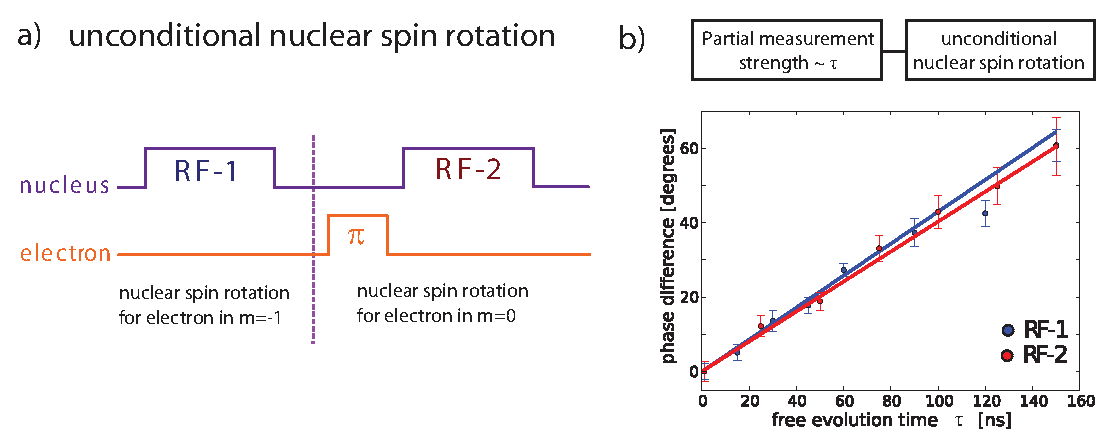
\includegraphics [width = 12 cm]{SOM/fig03_RFpulses_v2.eps}
\caption{\textit {On the left, pulse sequence for unconditional nuclear spin rotation. On the right, phase of the nuclear spin as a function of the free evolution time $\tau$, for the two electron-spin manifolds ($m_S=-1$ and $m_S=0$).}}
\label{fig:RF}
\end{figure} 



\section*{Partial measurements with controlled strength: Theory}
\label{sec:theory}
The protocol starts by initializing the nucleus in $\ket{\psi_N} = \frac{1}{\sqrt{2}} \left( \ket{\Downarrow}+\ket{\Uparrow} \right)$ and the electron in $\ket{\psi_e} = \ket{0}$.\\
The tunable-entangling gate consists of three steps. First, a $\pi/2$-pulse is applied around $x$ to the electron spin, creating the equal superposition state:
\begin{equation}
\left| \psi \right \rangle = \frac{1}{2} \left( \left| 0 \right \rangle - i \left| 1 \right \rangle \right) \left( \left| \Downarrow \right \rangle +\left| \Uparrow \right \rangle\right)
\end{equation}
Then the system undergoes free evolution of a variable time $\tau$ (according to the Hamiltonian in Eq. \ref{eq:H0_RWA}):
\begin{equation}
\ket{ \psi} = \frac{1}{2} \left \lbrace e^{0i} \ket{ 0, \Downarrow } + e^{-i A \tau} \ket{ 0, \Uparrow } - i  e^{-i A \tau/2} \ket{ 1, \Downarrow } - i  e^{-i A \tau/2} \ket{ 1, \Uparrow} \right \rbrace
\end{equation}
A second electron $\pi/2$-pulse, now around $y$, creates the state:
\begin{equation}
\left| \psi \right \rangle = \frac{1}{2} \left\lbrace \left| 0 \right \rangle \left[ \beta_+ (\tau) \left| \Downarrow \right \rangle + i e^{i A\tau/4} \beta_-(\tau) \left| \Uparrow \right \rangle \right] + e^{i\pi /2} \left| 1 \right \rangle \left[ \beta_-(\tau) \left| \Downarrow \right \rangle + i e^{i A\tau/4} \beta_+(\tau) \left| \Uparrow \right \rangle \right] \right\rbrace
\label{eq:state}
\end{equation}
where $\beta_{\pm} = \cos(\pi/4 \pm  A \tau/4)$. We define $\theta$ as $\theta= A \tau/2$, and the measurement strength as $\sin\theta$.\\
For $\theta=0$ ($\tau = 0$), the electron and nuclear spins are in a separable state:
\begin{equation}
\left| \psi (\tau=0) \right \rangle = \frac{1}{2} \left( \left| 0 \right \rangle +i \left| 1 \right \rangle \right) \left[ \left| \Downarrow \right \rangle +  i \left| \Uparrow \right \rangle \right]
\end{equation}
and a measurement of the electron spin gives no information about the state of the nuclear spin.
On the other hand, for $\theta = 90$ degrees (corresponding to $\tau = \pi/A = 229$ ns), the electron and nuclear spins are in a maximally-entangled state:
\begin{equation}
\left| \psi (\tau=\pi/A) \right \rangle = \frac{1}{\sqrt{2}} \left[ \left| 0, \Uparrow \right \rangle -i \left| 1, \Downarrow \right \rangle \right]
\end{equation}
and a measurement of the electron spin results in a projective measurement of the nuclear spin. Performing the electron-spin read-out by resonantly exciting the $E_y$ optical transition (therefore probing the population of the $\left| m_s=0 \right \rangle$ state) we project the nuclear spin on the $\left| m_I = -1 \right \rangle$ ($\ket{\Uparrow}$) state when a photon is detected and on the $\left| m_I = 0 \right \rangle$ ($\ket{\Downarrow}$) state when no photon is detected.\\
In the intermediate cases, $0<\tau<\pi/A$, the concurrence of the state as a function of $\tau$ is given by:
\begin{equation}
 C (\tau) = \sin\theta=\sin \left( A \tau/2 \right) 
\label{eq:concurrence}
\end{equation}
if $\ket{\psi_N}$ is initialized in $\ket{x}$. The value of C corresponds to the strength of the measurement performed on the system qubit.\\
Note from Eq. \ref{eq:state} that a $\tau$-dependent phase shift $\varphi = + A \tau/4$, unconditional on the electron spin, is imposed on the nuclear spin state after the measurement, as a result of the variable free evolution time. We compensate by adjusting the phase of the final RF pulse (see Section \ref{sec:uncond_rot_RF} for details).\\
The nuclear spin density matrix, unconditioned on the result of the electron spin measurement, can be derived by tracing over the electron spin, resulting in:
\begin{equation}
 \rho_{uncond} = \frac{1}{2}
 \left[
% \begin{center}
\begin{array}{cc}
1 & \cos^2 ( A \tau/2)\\
\cos^2 ( A \tau/2) & 1
 \end{array}
% \end{center}
 \right]
\label{eq:uncondRho}
 \end{equation}
Increasing the measurement strength, the initial pure state becomes increasingly mixed, resulting in a completely mixed state for $\theta = 90$ degrees.\\
 Conditioning on measuring the electron spin in the state $\ket{0}$, the nuclear spin state is:
\begin{equation}
 \rho_0 = \frac{1}{2}
 \left[
% \begin{center}
\begin{array}{cc}
1+\sin ( A \tau/2) & \cos^2 ( A \tau/2)\\
\cos^2 ( A \tau/2) & 1-\sin(A \tau/2)
 \end{array}
% \end{center}
 \right]
 \label{eq:condRho}
\end{equation}
Now, the resulting state remains pure, but it is increasingly rotated towards $\ket{\Uparrow}$ for increasing measurement strength. 

\section*{Characterization of the partial measurements}
\label{sec:charpartialmsmnt}
The partial measurement was characterized by performing quantum state tomography, as explained in the main text. In Fig \ref{fig:backaction}, we plot the elements of the density matrix of the nuclear spin after the partial measurement as a function of the measurement strength, for three different input states $\{ \ket{\Uparrow}, \ket{x}, \ket{y} \}$. On the upper row we do not take the measurement outcome of the electron into account, while on the lower row we show the data conditioned on the detection of a photon (ancilla projected to $\ket{0}$).\\
When we condition on a measurement result for the ancilla, the operation on the system qubit is a projection with increasing strength (completely projective along $z$ for measurement strength 1). In the unconditioned case, we observe measurement-induced dephasing.

\begin{figure} 
\includegraphics [width = 12 cm]{SOM/fig04_backAction.eps}
\caption{\textit{Density matrix elements of the states after a partial measurement, as a function of the measurement strength, for three different input states. On the upper row, data not taking the electron spin readout into account. On the lower row, data conditioned on detection of a photon (electron spin projected to $m_s = 0$). Solid lines represent theoretical prediction from Eq. \ref{eq:uncondRho} and Eq. \ref{eq:condRho}}}
\label{fig:backaction}
\end{figure} 


We characterized the collapse process by quantum process tomography \cite{Nielsen__2000}. Results are plotted in Fig. \ref{fig:QPT}. On the upper row, the process matrix for the unconditioned case shows a continuous transition from the identity process to a collapse process consisting of equal contributions of $\mathbb{\hat{1}}$ and $\hat{\sigma}_z$: the absence of off-diagonal terms represents the increasing dephasing. The theoretical process matrix for the unconditioned case is:
\begin{equation}
 \hat{\chi}_{uncond} = \frac{1}{2}
 \left[
\begin{array}{cccc}
1+\cos\theta & 0 & 0 & 0\\
0 & 0 & 0 & 0\\
0 & 0 & 0 & 0\\
0 & 0 & 0 & 1-\cos\theta
 \end{array}
 \right]
\end{equation}
On the bottom row, we plot the process conditioned on the measurement result of the electron spin: this is a non-trace-preserving process, with state-dependent success probability \cite{Bongioanni_Phys.Rev.A_2010}. The theoretical process matrix as a function of $\theta$ is:
\begin{equation}
\hat{\chi}_{cond} = \frac{1}{2}
 \left[
\begin{array}{cccc}
1+\cos\theta & 0 & 0 & \sin\theta\\
0 & 0 & 0 & 0\\
0 & 0 & 0 & 0\\
\sin\theta & 0 & 0 & 1-\cos\theta
 \end{array}
 \right]
\end{equation}
In this case, the process is coherent and the off-diagonal terms are, in general, non-zero. The fidelity between the ideal process matrix and our experimentally reconstructed one is plotted in Fig. \ref{fig:QPT_fid}.


\begin{figure} 
\centering
\includegraphics [width = 12 cm]{SOM/fig05_QPT.eps}
\caption{\textit{ Quantum process tomography for the tunable-strength measurement for different strength values (defined by the value of $\tau$ and the corresponding values for $\theta =  A \tau/2$ and measurement strength $C=\sin\theta$). On the upper row, the real part of the process matrix for the unconditioned case. On the lower row, the process matrix conditioned on a measurement of the ancilla giving the result $\ket{0}$.}}
\label{fig:QPT}
\end{figure} 


\begin{figure} 
\centering
\includegraphics [width = 6 cm]{SOM/fig06_QPTfidelity.eps}
\caption{\textit{ Fidelity of the reconstructed quantum process matrices $\chi_{cond}$ and $\chi_{uncond}$, as a function of the measurement strength ($C = \sin\theta$). The fidelity is calculated with the formula: $F (\chi_{exp}, \chi_{th})  = \mbox{Tr} \left \lbrace \sqrt{\sqrt{\chi_{exp}} \chi_{th} \sqrt{\chi_{exp}}} \right\rbrace^2$ \cite{Bongioanni_Phys.Rev.A_2010}.}}
\label{fig:QPT_fid}
\end{figure} 

\section* {Weak value and conditioned average}
\label{sec:weakvaluecondave}
Given an observable $\mathcal{I}$, the weak value of the associated quantum operator $\hat{I}$, as introduced by Aharonov, Albert and Vaidman \cite{Aharonov_PRL_1988,Kofman_PhysicsReports_2012}, is defined by

\begin{equation}
\label{eq:wv}
 I_W = \frac{ \bra{\psi_f} \hat{I} \ket{\psi_i}}{\left \langle \psi_f | \psi_i \right \rangle }
\end{equation}
This quantity does not depend on the context of the specific measurement, but only on the operator $\hat{A}$ and on the initial and final states (respectively $\left| \psi_i \right \rangle$ and $\left| \psi_f \right \rangle$). For a qubit, with initial state $\ket{\psi_i} = \ket{x}$ and final state $\ket{\psi_f}  = \cos \phi \ket{0} + \sin \phi \ket{1}$, we have $(S_z)_w = \cos 2\phi/(1+\sin 2\phi)$.\\
Given an observable $\mathcal{A}$, one can measure it with a series of operators, which can be projectors $\lbrace \hat{\Pi}_k , \hat{\Pi}_k^2 = \hat{\Pi}_k\rbrace$ or, more generally, POVMs $\lbrace \hat{E}_j = \hat{M}^{\dagger}_j \hat{M}_j \rbrace$. The associated measurement outcomes are, respectively, the eigenvalues $\left \lbrace a_k \right \rbrace$ and the generalized eigenvalues (or contextual values) $\left \lbrace \alpha_j \right \rbrace$ \cite{Dressel_Phys.Rev.Lett._2010}, such that the spectral decomposition of the operator $\hat{I}$ can be written as:
\begin{equation}
 \hat{I} = \sum_j \alpha_j \hat{E}_j = \sum_k a_k \hat{\Pi}_k
\end{equation}


Consider now a sequence of two measurements, $\mathcal{M}_1$ and $\mathcal{M}_2$ and suppose to condition the average of the result of  $\mathcal{M}_1$ to a measurement result for $\mathcal{M}_2$. The generalized weak value (or conditioned average) of the observable is defined as:
\begin{equation}
 _f \left \langle I \right \rangle = \sum_j \alpha_j^{(1)} P(j|f)
\end{equation}
where $\lbrace \alpha_j^{(1)}\rbrace$ are the possible measurement outcomes of $\mathcal{M}_1$ (generalized eigenvalues) and $P(j|f) = p_{jf}/(\sum_j p_{jf})$ is the conditional probability to detect the outcome $\alpha_j^{(1)}$ in the first measurement, given the outcome $\alpha_f^{(2)}$ for the second measurement.\\
Unlike the weak value, the conditioned average encodes information not only about the observable $\mathcal{A}$, but also on the specific measurement context. However, it can be shown \cite{Dressel_Phys.Rev.Lett._2010} that, under certain conditions (namely minimal state disturbance), the dependence on the measurement vanishes. For a pure initial state, a pure POVM and a projective final measurement, it reduces to the weak value of Eq. \ref{eq:wv} .\\
In our case, for a measurement operator $\hat{E}_j = (1/2) (\mathbb{\hat{1}} \pm \sin\theta \hat{I}_z)$, the generalized eigenvalues are $\pm 1/\sin\theta$ and the conditional average is:
\begin{equation}
\label{eq:cond_avg}
 _f \left \langle I_z \right \rangle = \frac{1}{\sin\theta} \frac{p_{00}-p_{10}}{p_{00}+p_{10}}  = \frac{\cos 2\phi}{1+ \cos \theta \sin 2\phi}
\end{equation}
This quantity reduces to the quantum weak value for $\sin\theta = 0$ and does not diverge for finite measurement strength. Note that from this expression \cite{Williams_PRL_2008,Groen_PRL_2013}, it is possible to observe values lying outside the range of the operator eigenvalues for any finite measurement strength.
\\

\section* {Experimental quantum weak value for a spin qubit}
A measurement of the conditional average $ _f \left \langle I_z \right \rangle$ is performed with the pulse sequence shown in Fig. \ref{fig:amc-fig1}a of the main text, starting from the initial state $\ket{x} = (1/\sqrt{2}) \left( \ket{\Downarrow} + \ket{\Uparrow} \right)$. The scheme consists of a partial measurement (strength $\theta$) followed by a projective measurement in a rotated basis (angle $\phi$), post-selecting on the result of the projective measurement. In the first set of measurements (large panel in Fig. \ref{fig:amc-fig2}d of the main text) we fix the strength of the first measurement and sweep the basis rotation angle $\phi$ before the projective measurement. For the inset of Fig. \ref{fig:amc-fig2}d of the main text we sweep the measurement strength $\theta$ and choose $\phi$ to yield the maximum weak value. \\
We post-select on the measurement outcome $\ket{0}$ for the ancilla read-out (system in $\ket{\Uparrow}$), corresponding to the detection of a photon (electron spin in $m_s=0$). \\
The conditional average can be calculated with the expression in Eq. \ref {eq:cond_avg} where $p_{ij}$ is the probability of outcome $i$ for the ancilla read-out of the partial measurement and measurement outcome $j$ for the ancilla read-out of the projective measurement (assuming perfect readout). From Eq. \ref{eq:state}, we calculate the dependence of $p_{ij}$ on $\phi$ and $\theta$:
\begin{equation}
\label{eq:prob_wm}
  \begin{split}
  p_{11}&=\frac{1}{2} \left[ \beta_-(\theta) \cos\phi + \beta_+ (\theta) \sin\phi \right]^2  \\
  p_{10}&= \frac{1}{2} \left[ \beta_-(\theta) \sin\phi - \beta_+ (\theta) \cos\phi\right]^2 \\
  p_{01}&= \frac{1}{2} \left[ \beta_-(\theta) \sin\phi + \beta_+ (\theta) \cos\phi\right]^2 \\
  p_{00}&=\frac{1}{2} \left[ \beta_-(\theta) \cos\phi - \beta_+ (\theta) \sin\phi \right]^2 
  \end{split}
\end{equation}
where $\beta_{\pm} (\theta) = \cos (\pi/4 \pm \theta/2)$.\\
 
Since our read-out is not perfect, it must be calibrated to take into account the finite detection efficiency and the dark counts. For the state $m_s=0$ we are limited by our detection efficiency ($\sim .80$), while for the $m_s=-1$ read-out we suffer from dark counts. We define $F_i$ as the fidelity of the $m_s=0$ read-out and $G_i$ as the read-out fidelity for $m_s=-1$, in the $i-$th measurement.
Then, given the ideal probabilities $p_{ij}$, the measured fractions $n_{ij}$ are:
 
\begin{equation}
\resizebox{.9\hsize}{!}{$
\left[
\begin{array}{c}
n_{11}\\
n_{10}\\
n_{01}\\
n_{00}
 \end{array}
 \right]=
 \left[
\begin{array}{cccc}
G_1 G_2 & G_1(1-F_2) & (1-F_1)G_2 & (1-F_1)(1-F_2)\\
G_1(1-G_2) & G_1 F_2 & (1-F_1)(1-G_2) & F_2(1-F_1)\\
(1-G_1)G_2 & (1-G_1)(1-F_2) & F_1 G_2 & F_1(1-F_2)\\
(1-G_1)(1-G_2) & (1-G_1)F_2 & F_1 (1-G_2) & F_1 F_2
 \end{array}
 \right]
\left[
\begin{array}{c}
p_{11}\\
p_{10}\\
p_{01}\\
p_{00}
 \end{array}
 \right] $}
\label{ROcor}
\end{equation}
The theoretical curve in Fig. \ref{fig:amc-fig2}d of the main text is calculated without fit-parameters, using the read-out correction of Eq. \ref{ROcor} and assuming an asymmetric spin-flip rate $f= 0.02$ between the first and second read-out. This spin-flip probability arises during the reset of the ancilla by optically exciting the forbidden transition of Ey. The value $f$ is determined from independent measurements. \\


\section*{Partial measurements as probabilistic rotations}
Starting from the state $\ket{\psi_{init}} =  \cos\theta_i \ket{\Downarrow}+ \sin\theta_i \ket{\Uparrow} $, we perform a partial measurement with strength $\theta_m$. With probability $\cos^2\theta$, we obtain the state:
\begin{equation}
 \ket{\psi_0} = \frac{1}{\mathcal{N}_0} \left[ \cos \left( \pi/4 + \theta_m/2 \right) \cos\theta_i \ket{\Downarrow} +  \cos \left( \pi/4 - \theta_m/2 \right) \sin\theta_i \ket{\Uparrow} \right]
\end{equation}
where $1/\mathcal{N}_0$ is the normalization factor. The state, initially at an angle $\theta_i$, is rotated to the angle:
\begin{equation}
 \theta_0 = \arctan{ \left[ \tan\theta_i \frac{\cos\theta_m}{1-\sin\theta_m} \right]}
\end{equation}
On the other hand, with probability $p_{succ} = \sin^2\theta$, the measurmeent leads to the state:
\begin{equation}
 \ket{\psi_1} = \frac{1}{\mathcal{N}_1} \left[ \cos \left( \pi/4 - \theta_m/2 \right) \cos\theta_i \ket{\Downarrow} +  \cos \left( \pi/4 + \theta_m/2 \right) \sin\theta_i \ket{\Uparrow} \right]
\end{equation}
Therefore, the initial state rotated to the angle:
\begin{equation}
 \theta_1 = \arctan{ \left[ \tan\theta_i \frac{1-\sin\theta_m}{\cos\theta_m} \right]}
\end{equation}
In other words, as shown in \cite{Jordan_PRB_2006}, a partial measurement is equivalent to a probabilistic state rotation, with a rotation angle which depends on the strength of the measurement and on the initial state (see Fig. \ref{fig:prob_rot}).

\begin{figure} 
\centering
\includegraphics [width = 12 cm]{SOM/fig07_prob_rotation.eps}
\caption{\textit{A partial measurement is equivalent to a probabilistic rotation. Given a an initial superposition with angle $\theta_i$ ($\ket{\psi_{init}} =  \cos\theta_i \ket{\Downarrow}+ \sin\theta_i \ket{\Uparrow} $) and a partial measurement with strength $\theta_m$, one gets the rotation angle plotted on the upper left subplot in case the electron spin is measured to be in $\ket{0}$ (probability $\cos^2 \theta_i$, plot on the bottom left) or the rotation angle plotted on the upper right in case the electron spin is measured to be in $\ket{1}$ (probability $\sin^2 \theta_i$, plot on the bottom right)}}
\label{fig:prob_rot}
\end{figure} 


\section*{Heralded sequential measurements: un-collapse and steering}
In Fig. \ref{fig:uncollapse}, we implement two heralded sequential partial measurements. We post-select on the case of photon detection, using short read-out times to minimize electron spin-flips, at the price of reduced success probabilities. We can do this with high fidelity, maintaining a good coherence of the state after two measurements. No spin-pumping between the two measurements is performed, in order to avoid electron spin-flips that would destroy nuclear-spin coherence.\\
We first perform a measurement with strength $\theta_1=20$ degrees, followed by a measurement with the same strength but projecting on the opposite electron state (equivalent to a measurement with strength $\theta_2=-20$ degrees). This brings us back to the original quantum state, in a probabilistic un-collapse of the state. This technique has been used to probabilistically recover a state subject to amplitude-damping decoherence \cite{Koashi_Phys.Rev.Lett._1999,Korotkov_Phys.Rev.Lett._2006,Katz_Phys.Rev.Lett._2008}.  \\
In general, a partial quantum measurement is equivalent to a probabilistic rotation. For $\theta_1=\theta_2=+20$ degrees, two successive measurements result in a combined rotation of $39$ degrees, with success probability $0.16$. In our case, heralding on photon detection, this can be done quite effectively (fidelity $0.78$).

\begin{figure} 
\centering
\includegraphics [width = 12 cm]{SOM/fig08_uncollapse.eps}
\caption{\textit{Two sequential heralded partial measurements, both post-selected on the case of photon detection. The density matrices are the result of state tomography, performed after the two partial measurements. For the uncollapse (upper density matrix), first a measurement with strength $C = 0.34$ ($\theta_1=20$ degrees) is performed, after which the initial state is restored by a second measurement with $\theta_2 = -20$ degrees. For the lower density matrix, the second measurement is set to  $\theta_2 = 39$ degrees, such that the system, that was projected towards $|\downarrow >$ after the first measurements,  is steered towards $|\uparrow >$ through the backaction of the second measurement.}}
\label{fig:uncollapse}
\end{figure} 

\section*{State steering by real-time adaptive measurements}
\label{sec:steeringpartmsmnt}
\subsection*{Ideal protocol}
We start in the state $\left| \psi_0 \right \rangle = \ket{x} = (1/\sqrt{2}) \left(\left| \Downarrow \right \rangle + \left| \Uparrow \right \rangle \right)$, with the goal to reach a target state $\left| \psi_T \right \rangle = \cos\theta_T \left| \Downarrow \right \rangle + \sin\theta_T \left| \Uparrow \right \rangle$.\\
First, we do a measurement with strength $\theta_1 = \pi/2-2\theta_T$. With probability $0.5$ the system reaches the target state, while in the rest of the cases it is shifted in the oppposite direction, to the state:
\begin{equation}
\left| \psi_1 \right \rangle = \cos \left( \frac{\pi}{4} - \frac{\theta_1}{2} \right) \left| \Downarrow \right \rangle + \cos \left( \frac{\pi}{4} + \frac{\theta_1}{2} \right) \left| \Uparrow \right \rangle
\end{equation}
In order to try to steer it back, we perform a second measurement, with strength $\theta_2$. In case of success, we get the state:
\begin{equation}
\resizebox{.9\hsize}{!}{$
\left| \psi_{10} \right \rangle = \frac{1}{\mathcal{N}} \left[ \cos \left( \frac{\pi}{4} - \frac{\theta_1}{2} \right)\cos \left( \frac{\pi}{4} + \frac{\theta_2}{2} \right) \left| \Downarrow \right \rangle + \cos \left( \frac{\pi}{4} + \frac{\theta_1}{2} \right)\cos \left( \frac{\pi}{4} - \frac{\theta_2}{2} \right) \left| \Uparrow \right \rangle \right]
$}
\end{equation}
where $\mathcal{N} = \left[ \cos^{2} \left( \frac{\pi}{4} - \frac{\theta_1}{2} \right)\cos^2 \left( \frac{\pi}{4} + \frac{\theta_2}{2} \right) + \cos^2 \left( \frac{\pi}{4} + \frac{\theta_1}{2} \right) \cos^2 \left( \frac{\pi}{4} - \frac{\theta_2}{2} \right) \right]^{1/2}$.
The system can be steered to target state, by setting:
\begin{equation}
 \frac{1}{\mathcal{N}} \cos \left( \frac{\pi}{4} - \frac{\theta_1}{2} \right)\cos \left( \frac{\pi}{4} + \frac{\theta_2}{2} \right) = \cos \left( \frac{\pi}{4} + \frac{\theta_1}{2} \right)
\end{equation}
After simplification, this leads to the equation:
\begin{equation}
\left( 1 + \sin \theta_1 \right) \left( 1 - \sin \theta_2 \right) = \left( 1 - \sin \theta_1 \right) \left( 1 - \sin \theta_1 \sin \theta_2 \right)
\end{equation}
Solving for $\theta_2$, we find that the strength of the second measurement can be tuned as:
\begin{equation}
 \theta_2 =  \sin^{-1} \left[ 2\frac{\sin \theta_1}{1+\sin^2 \theta_1} \right]
\end{equation}
The probability to steer the state to the desired target, after two measurements, is:
\begin{equation}
 p_{success} = \frac{ 1 + \cos \theta_1 }{2}
\end{equation}


\begin{figure} 
\centering
\includegraphics [width = 12 cm]{SOM/fig09_adaptMsmsnt_angle.eps}
\caption{\textit{On the left, strength of the second measurement, as a function of the desired target state. On the right, success probability of the two-step algorithm.}}
\label{}
\end{figure} 


\subsection*{Error analysis}
The protocol described in the last Section assumes ideal measurements. In practice, however, we are subject to several non-ideal conditions \cite{Robledo_Nature_2011}:
\begin{itemize}
 \item the electron-spin read-out is not perfect. Given that the electron is in $m_s=0$, if we excite the $E_{y}$ transition, we are supposed to detect photons. However, such photons are detected with a finite efficiency (due to losses in the diamond, the collection optics and the finite efficiency of the detector). This results in a read-out fidelity $F_0 < 1$. In the first measurement, this leads us to make the wrong decision and apply a correction although we had already reached the target state.
 \item due to dark counts, we detect photon clicks even in the absence of photons. This probability is quite small, so we neglect it in the following analysis
 \item during electron read-out, there is a probability ($q$) that the electron spin flips. This results in dephasing of the nuclear spin. Moreover, with a small probability it results also in a nuclear spin-flip (we measured the probability to get a nuclear spin-flip as a result of an electron spin-flip to be around $0.02$). We neglect the nuclear spin flip and just consider the effect of dephasing.
\end{itemize}

The read-out efficiency and spin-flip probability are not independent: the longer the read-out, the higher the detection efficiency, but, at the same time, the electron spin-flip probability is also increased. The read-out fidelity $F_0$ and the electron spin-flip probability $q$, as a function of read-out time, are shown in the inset of Fig. \ref{fig:adaptiveScheme}. The best trade-off is for a read-out time $T \sim 5 \mu$s, where $F_0 \sim 0.6$ and $q \sim 0.2$.

\begin{figure} 
\centering
\includegraphics [width = 12 cm]{SOM/fig10_adaptiveScheme.eps}
\caption{\textit{Description of the adaptive scheme. Ancilla readout $\ket{0}$ corresponds to the detection of a photon when optically exciting the $E_{y}$ transition, while no photon detection corresponds to ancilla projection to $\ket{1}$. Inset: experimental data for electron spin read-out fidelity $F_0$ and spin-flip probability $q$ as a function of read-out time.}}
\label{fig:adaptiveScheme}
\end{figure} 

We prepare the initial $\ket{x}$ state and perform the first measurement. With probability $p_C = 0.5 F_0$, the ancilla readout outcome is $\ket{0}$ (corresponding to a photon detection event) and we take the upper branch of Fig. \ref{fig:adaptiveScheme}. The resulting density matrix is:
\begin{equation}
\begin{split}
 \rho_C &= (1-q) \ket{\psi_0}\bra{\psi_0} + q \rho_0^{(deph)}\\
 &= \frac{1}{2} \left[
\begin{array}{cc}
1-\sin\theta_1 & (1-q) \cos\theta_1\\
(1-q) \cos\theta_1 & 1+\sin \theta_1
\end{array}
\right]
\end{split}
\end{equation}

The density matrix $\rho^{(deph)}$ is the completely-mixed equivalent of the density matrix $\rho$, with zero off-diagonal elements. 
For no electron spin-flips ($q = 0$) this would just be the density matrix of the pure target state.
On the other hand, for perfect ancilla readout fidelity ($F_0=1$), the measurement outcome $\ket{1}$ would lead to the following density matrix (in the lower branch of Fig. \ref{fig:adaptiveScheme}):
\begin{equation}
\begin{split}
 \rho_W &= (1-q) \ket{\psi_1}\bra{\psi_1} + q \rho_1^{(deph)}\\
&=
\frac{1}{2}
\left[
\begin{array}{cc}
1+\sin\theta_1 & (1-q) \cos\theta_1\\
(1-q) \cos\theta_1 & 1-\sin \theta_1
\end{array}
\right]
\end{split}
\end{equation}

However, we get into the lower branch of Fig. \ref{fig:adaptiveScheme} also when we are supposed to get the outcome $\ket{0}$ but, due to the imperfect read-out (fidelity $F_0<1$), we missed the corresponding photon, which lead us to believe that the measurement outcome was $\ket{1}$. Taking this into account, the density matrix results for ancilla measurement outcome $\ket{1}$ is composed by two terms:
\begin{equation}
 \rho_N \sim 0.5 \rho_W + 0.5 (1-F_0) \rho_C
 \label{eq:rhoN}
\end{equation}
The total probability to be in the lower branch of Fig. \ref{fig:adaptiveScheme} is $p_W = 1- 0.5 F_0$.\\
If we are in the lower branch, we try to reach the target state by performing a second measurement, which is successful (ancilla projected to $\ket{0}$) with probability $p_1 (\theta_1)$. In this case, the component $\rho_W$ is rotated back to the target state, with some spin-flip probability and the corresponding dephasing:
\begin{equation}
 \rho_{W}' = (1-q) \left[ (1-q) \ket{\psi_0}\bra{\psi_0} + q \rho_0^{(deph)} \right] +q \rho_1^{(deph)}
\end{equation}
The component $\rho_C$ is, on the other end, rotated in the wrong direction:
\begin{equation}
  \rho_{C}' = (1-q) \left[ (1-q) \ket{\psi_2}\bra{\psi_2} + q \rho_2^{(deph)} \right] +q \rho_0^{(deph)}
 \label{eq:rho1c}
\end{equation}

The density matrix, for ancilla measurement outcome $\ket{1}$ in the second measurement is:
\begin{equation}
 \rho_{NC} = \frac{1}{1-0.5F_0} \left[ 0.5 \rho_W' + 0.5 (1-F_0) \rho_C' \right]
\end{equation}
%where $\rho_{deph} = q \left[ \rho_0^{(deph)} +(1-F_0) \rho_2^{(deph)} \right] +q \rho_1^{(deph)}$.
It consists of three terms: a contribution $\ket{\psi_0}\bra{\psi_0}$ which has been correctly recovered by the adaptive measurement, an error contribution $\ket{\psi_2}\bra{\psi_2}$ (due to wrong feedback) and a dephased contribution (due to imperfect read-out).\\
The density matrix $\rho_{succ}$, taking into account the cases where our protocol heralds success (so either detecting a photon in the first measurement, or only detecting a photon in the second measurement) is:
\begin{equation}
\rho_{succ} = \frac{1}{p_1 + 0.5 F_0} \left[  0.5 F_0  \rho_C + p_1 \rho_{NC} \right]
\end{equation}


The state fidelity is then calculated as $\mathcal{F} = \bra{\psi_0} \rho_{succ} \ket{\psi_0}$.
\begin{figure} [H]
\centering
\includegraphics [width = 12 cm]{SOM/fig11_adaptiveScheme_normalRO.eps}
\caption{\textit{Realistic model for the adaptive scheme. On the left, density matrix elements for the different states in Fig. \ref{fig:adaptiveScheme}. On the right, success probabilities and state fidelity as a function of electron spin read-out time.}}
\label{fig:sim_adapt_fullRO}
\end{figure} 
The results of the simulation are plotted in Fig. \ref{fig:sim_adapt_fullRO}. For each of the four plots on the left, we show the three elements of the density matrix ($\rho_{00}$, $\rho_{01}$ and $\rho_{11}$). \\

For measurement outcome $\ket{0}$ in the ancilla readout in the first measurement, we take the upper branch in the scheme in Fig. \ref{fig:adaptiveScheme}, resulting in the density matrix $\rho_C$. This density matrix shows correct values for the $z$-components, independently of the read-out time. Increasing the read-out time, we increase the probability of taking the upper branch, up to a maximum value $0.5 \times 0.8 = 0.4$, in the case $F_0=0.8$. However, the dephasing also increases, together with the success probability, as shown on the right plot (green curve, success probability measurement-1). \\
For measurement outcome $\ket{1}$, we take the lower branch and get the state described by the density matrix $\rho_N$. The elements of $\rho_N$ (Eq. \ref{eq:rhoN}) are, as expected, the opposite of the target state: for longer read-out time, however, they do not saturate to the exact opposite value, since there is also a component of state that would be the correct one, but is in the wrong branch because the associated photons were not detected.\\
Considering the second measurement, ancilla measurement outcome $\ket{0}$ leads us to $\rho_{NC}$. In this case, we manage to invert the matrix elements and restore a density matrix more similar to the target one, but not completely because the restoring transformation has been also applied to the correct component, making it wrong (state described by $\rho_C'$ in Eq. \ref{eq:rho1c}). \\
Combining $\rho_C$ and $\rho_{NC}$, we get $\rho_{succ}$. Two features are important: the longer the read-out time, the higher read-out fidelity and therefore the more frequently the right choice is made in the adaptive step. This reflects in a higher fidelity of the $z$ components of the density matrix and higher success probability (red curve on the right plot). On the other hand, for longer read-out time, the probability of ancilla spin-flips is higher, which results in increasing dephasing. In the right plot, this is clear from the trade-off between state fidelity and success probability.

\begin{figure} 
\centering
\includegraphics [width = 12 cm]{SOM/fig12_results_normalRO.eps}
\caption{\textit{Experimental results for success probability (on the left) and state fidelity (on the right) for the adaptive measurement protocol, using full electron-spin read-out}}
\label{fig:exp_adapt_fullRO}
\end{figure} 

In Fig. \ref{fig:exp_adapt_fullRO}, we plot the experimental results obtained using full electron-spin read-out. Compared to the results reported in the main text (Fig. 4, dynamical-stop read-out), the state is completely dephased after about $20 \mu$s and the fidelity decreases quickly to around $0.6$.

\subsection*{Dynamical-stop electron read-out}


As described in the main text, dynamical-stop electron spin read-out allows us to reduce the dephasing on the nuclear spin induced by electron measurement. To model the effect of dynamical-stop read-out we take the assumption that read-out stops as soon as a photon is detected, causing no electron spin-flip and no nuclear-spin dephasing. The assumption of no nuclear-spin dephasing is not confirmed by experimental data in Fig. 3c of the main text: however, it is justified to use it here for a simple model that gives a higher bound on the expected fidelity. \\

The results of the model for dynamical-stop read-out are reported in Fig. \ref{fig:model_segmRO}. Compared to Fig. \ref{fig:sim_adapt_fullRO}, the state $\rho_C$ is not dephased, while $\rho_N$ is similar to the one for full read-out. This results, in a much less dephased state in case of success ($\rho_{succ}$). The fidelities for the case when using full electron-spin read-out or dynamical-stop read-out are plotted on the right side of Fig. \ref{fig:model_segmRO}.
\begin{figure} [h]
\centering
\includegraphics [width = 12 cm]{SOM/fig13_adaptiveSceheme_dynStopRO.eps}
\caption{\textit{Model of the adaptive scheme results, using dynamical read-out. On the left, density matrix elements for the states at different stages of the protocol on Fig. \ref{fig:adaptiveScheme}. On the right, comparison between state fidelity using conventional electron read-out and dynamical-stop read-out.}}
\label{fig:model_segmRO}
\end{figure} 


\newpage
\bibliographystyle{../thesis}
\setcounter{tocdepth}{1}
\bibliography{amc_appendix}



\graphicspath{{./ch_LDE_SI/figures/}}

\chapter{Heralded entanglement}
\label{ch:LDEappendix}


\section{Setup}
We perform the experiments with two home-built low-temperature confocal microscopes. Each setup features lasers for off-resonant and resonant excitation, cryogenic piezoelectric positioners and high-efficiency/low background fluorescence detection paths. The zero-phonon line (ZPL) detection paths of both setups lead to the common beam splitter and photon detectors used for the entanglement generation. Each setup has an independent microwave (MW) source (Rohde \& Schwarz SMB100A) and MW amplifier (Amplifier Research 20S1G4 and AR 40S1G4 for setups A and B, respectively) to drive the NV centre electron spins.

Sample A is mounted on a XYZ stepper/scanner piezo stack (Attocube) in a Janis ST-500 flow cryostat and kept at $T \approx 8$\,K. Sample B is mounted on a XYZ stepper (Attocube) inside a custom-built Cryovac bath cryostat with optical access and kept at a temperature of $T \approx 4$\,K. 

Off resonant green excitation is provided for each of the setups by 532\,nm lasers (Spectra Physics Millenia Pro and Laser 2000 Cobalt Samba for setups A and B, respectively). Two tuneable 637\,nm lasers (New Focus Velocity) for independent resonant excitation are used for optical spin-pumping. For  the resonant excitation pulses used to generate the entanglement both setups share a tuneable continuous wave 637\,nm laser (Sirah Matisse DS). Its output is sequentially fed through an acousto-optic modulator (AOM; Crystal Technologies) and an electro-optic modulator (EOM; Jenoptik). After passing through the AOM \& EOM, the beam is split using a 50/50 beam splitter, and a 30 cm adjustable delay line is inserted in one arm for fine-tuning the temporal overlap of the excitation.

The photon emission of each NV is split into a ZPL part and an off-resonant phonon sideband (PSB) part by a dichroic long-pass filter (Semrock LPD01-633RS). The PSB emission is independently detected for each setup by avalanche photo-diodes (APDs; Perkin-Elmer SPCM). The ZPL emission is further filtered by a second dichroic filter (to remove green excitation light) and a tuneable band pass filter (Semrock TBP-700B). After filtering resonant excitation light by cross-polarisation rejection the ZPL emission of NVs A and B is coupled into the input ports of a fibre-coupled beam splitter (Evanescent Optics) by polarisation-maintaining fibres. The photons leaving the output ports of the beam splitter are detected by fibre-coupled avalanche photo-diodes (Picoquant Tau-SPAD) and time-tagged by a Picoquant Hydraharp 400 system.

\section{Rejection of resonant excitation light}
The experimental protocol requires the resonant excitation of a single optical transition and the detection of indistinguishable resonant photons from spontaneous emission of this transition. We use polarisation rejection and time-filtering to filter residual resonant excitation light --- stemming from reflections from optical elements and the sample surface --- from the signal.

The excitation laser is linearly polarised and rotated using a half-wave-plate (HWP) to a non-zero angle $\varphi$  with respect to the (linear) dipole of the $\ket{\up}\leftrightarrow\ket{E_y}$ transition it excites (Fig.\,\ref{fig:resonant_detection}). In the detection path, the combination of a half-wave plate and polariser sets a detection axis with an angle $\theta$ in the opposite direction with respect to the NV transition dipole. A further quarter-wave-plate (QWP) corrects for circular polarisation components of the signal that are induced by optical elements in the detection path.  We find the optimum in laser-rejection, NV excitation efficiency and NV collection efficiency by varying the angles $\varphi,\theta$ while keeping $\varphi + \theta = 90^\circ$.
% $\varphi=\theta=45^\circ$ will reject the laser reflections while reducing the NV collection efficiency by half.

As can be seen in Fig.\,\ref{fig:laser_vs_nv}, reflections of the two-nanosecond excitation pulse can be clearly distinguished from the exponentially decaying NV centre emission. In this manner laser reflections that are not removed by the polarisation rejection can be removed by time-filtering. %We note that because of the detector dead-time it is only possible to detect one photon per excitation pulse, therefore a combination of polarisation rejection and time filter is required. 
\begin{figure}[h]
\centering
\includegraphics[width=10cm]{resonant_excitation_detection_gerwin.pdf}
\caption{Resonant detection and excitation. \textbf{a}, Working principle of cross-polarisation rejection. \textbf{b}, Optical setup. See text for details.}
\label{fig:resonant_detection}
\end{figure}

\section{Experimental control}
For the experiment to be feasible, a high repetition rate of the entanglement generation sequence is crucial, because the success probability per shot is small, $P_\mathrm s = 1/2 \times \eta_\mathrm A\eta_\mathrm B \approx 10^{-7}$. We achieve a reasonable repetition rate by employing a conditional protocol as follows (Fig.\,\ref{fig:conditional_measurement}): We first ensure that both NV centres are in the negative charge state and on resonance. To this end we independently re-set the charge and resonance state of the two NVs with green laser pulses until the resonant excitation lasers are on resonance \cite{Robledo:2011fs,Pfaff:2012ue}. After this preparation we run the spin-preparation and entanglement generation sequence. In case of successful generation of entanglement we read out both spins in a single shot and return to the charge and resonance (CR) check. Otherwise, we repeat spin-preparation and entanglement generation. After 300 unsuccessful entanglement attempts we start over with the CR check. The success probabilities for passing the CR check, $P_\mathrm{CR} \approx 2\%$, and for successfully generating entanglement let us predict an entanglement generation rate of $\sim 1/10\,\mathrm{minutes}$. For comparison, an unconditional protocol in which charge/resonance and entanglement generation are only verified in post-processing would yield an entanglement rate of only $\sim 1/50\,\mathrm{hours}$.

\begin{figure}[h]
\centering
\includegraphics[width=\textwidth]{conditional.pdf}
\caption{The conditional sequence to implement the entanglement protocol. Two programmable micro-controllers with integrated DAC- and counter modules ({\em ADwin 2x})  independently initialise each NV centre and perform the charge-resonance check described in the main text. If both checks pass, a trigger is sent to the Arbitrary Waveform Generator ({\em AWG}) that executes the entanglement protocol. The protocol is run up to 300 times until it is successful. A successful attempt is recognised by a logic device ({\em CPLD}) that looks for a success-signature in the stream of photon clicks produced, and sends a halt trigger to the AWG when it does. The readout is then performed by the ADwins, after which the sequence starts over.}
\label{fig:conditional_measurement}
\end{figure}

Conditional operation is implemented in the following manner: The CR check and readout is done independently for the two setups by two programmable micro-controllers with DAC- and counter modules (Adwin Gold II and Adwin Pro II for setup A and B, respectively). Once both CR checks pass, a start trigger is sent to the Arbitrary Waveform Generator (Tektronix AWG 5014C) that sequentially executes the entanglement protocol up to 300 times. For each round, the photon clicks are recorded and time-tagged by a Picoquant Hydraharp 400 system. In addition, the photon clicks are also monitored in real time by a programmable logic device (CPLD; Altera Max V development kit) that time-filters the signal and recognises a successful entanglement event; if a success occurs, a stop trigger is sent to the AWG within 50\,ns to prevent it from running the next entanglement cycle. Furthermore, the logic device triggers both ADwin micro controllers to start their readout sequence. Further (more selective) time filtering is done in post-processing for the successful events, by combining the time-tagged data and spin readout data.

\section{Optical Rabi oscillations}
On resonance (i.e. in the absence of quasi-static spectral diffusion), the exponential damping time $\tau_{\text{rabi}}$ of the Rabi oscillations is determined by the pure optical dephasing time $T_2^{*,\text{opt}}$ via\cite{Robledo2010}
\be
\frac{1}{\tau_{\text{rabi}}}=\frac{3}{4 T_1} + \frac{1}{2T_2^{*,\text{opt}}},
\ee
where $T_1$ is the NV centre optical lifetime (about 12 ns).

As can be seen in Fig.\,2b in the main text, and Fig.\,\ref{fig:cr_nv_B}, $\tau_{\text{rabi}}$ saturates to the lifetime-limited value for high thresholds. Similar saturation behaviour is observed for different optical Rabi frequencies.

\begin{figure}[h]
\centering
\includegraphics[width=5cm]{cr_NV_B.pdf}
\caption{Line-narrowing effect of the dynamical initialization of charge and resonance for NV B, exemplified by the dependence of the decay time of optical Rabi oscillations on preparation threshold. See Fig.\,2b in the main text for details of the pulse sequence used.}
\label{fig:cr_nv_B}
\end{figure}


\section{Fidelity measure}

We want to estimate the fidelity of the generated two-spin state $\ket{\psi}$ with respect to the ideal Bell state. We take the example of the Bell state $\Psi^+$:
\begin{equation}
\ket{\Psi^+} = (\ket{\uparrow}_\mathrm{A}\ket{\downarrow}_\mathrm{B} + \ket{\downarrow}_\mathrm{A}\ket{\uparrow}_\mathrm{B})/\sqrt{2} \equiv (\ket{\uparrow\downarrow}+\ket{\downarrow\uparrow})/\sqrt{2} ,
\end{equation}
where $\ket{\uparrow}$ and $\ket{\downarrow}$ denote the $\mszero$ and $\msmone$ spin sub-levels of the NV centre ground state and subscripts A, B indicate the two NV centres used. The density matrix for this state is
\begin{equation}
\rho_{\Psi^+} = \ket{\Psi^+}\bra{\Psi^+} = \frac{1}{2}\left(
\begin{array}{cccc}
 0 & 0 & 0 & 0 \\
 0 & 1 & 1 & 0 \\
 0 & 1 & 1 & 0 \\
 0 & 0 & 0 & 0
\end{array}
\right).
\end{equation}
The fidelity of the state $\ket{\Psi^+}$ with density matrix $\rho$, for both spins in the z-basis, is therefore
\begin{equation}
\mathcal{F} = \bra{\Psi^+}\rho\ket{\Psi^+} = \frac{1}{2}(\rho_{22}+\rho_{33}+\Re(\rho_{23})+\Re(\rho_{32})) = \frac{1}{2}(\rho_{22}+\rho_{33}+ 2\Re(\rho_{23})).
\end{equation}
The term coming from the diagonal elements, $\rho_{22} + \rho_{33}$, is given by the fraction of spin-readouts in which the outcomes from NVs A and B are anti-correlated. To estimate the off-diagonal terms we measure both spins in the X-basis by applying $\pi/2$-rotations around $\mathbf y$, yielding the density matrix
\begin{equation}
\tilde{\rho} = \left ( \sqrt{Y}\otimes\sqrt{Y} \right ) \rho \left ( \sqrt{Y}^{\dagger}\otimes\sqrt{Y}^{\dagger} \right ),
\end{equation}
where the operator $Y$ describes a $\pi$-rotation around the y-axis, 
\be
\sqrt{Y} = \mathrm e^{-\frac{\mathrm i}{\hbar} S_\mathrm y \pi/2},
\ee
where $S_\mathrm y$ is the y-component of the spin-$\frac{1}{2}$ operator. The contrast between measured correlations and anti-correlations in this basis is
\begin{equation}
\tilde{\rho}_{11}+\tilde{\rho}_{44}-\tilde{\rho}_{22}-\tilde{\rho}_{33} = 2\Re(\rho_{23})+2\Re(\rho_{14}).
\end{equation}
It follows from the definition of the density matrix that the absolute of $\Re(\rho_{14})$ is bounded by
\begin{equation}
\mid \Re(\rho_{14}) \mid \leq \sqrt{\rho_{11}\rho_{44}},
\end{equation}
and therefore
\begin{equation}
2\Re(\rho_{23}) \geq \tilde{\rho}_{11}+\tilde{\rho}_{44}-\tilde{\rho}_{22}-\tilde{\rho}_{33} - 2\sqrt{\rho_{11}\rho_{44}}.
\end{equation}
In terms of measured quantities in two bases, the fidelity has thus a strict lower bound of\cite{Blinov2004a}
\begin{equation}
\label{eq:fidlowerbound}
\mathcal{F} \geq \frac{1}{2}\left(\rho_{22}+\rho_{33}+\tilde{\rho}_{11}+\tilde{\rho}_{44}-\tilde{\rho}_{22}-\tilde{\rho}_{33} - 2\sqrt{\rho_{11}\rho_{44}}\right).
\end{equation}
The treatment for the Bell state $\ket{\Psi^-} = (\ket{\uparrow\downarrow}-\ket{\downarrow\uparrow})/\sqrt{2}$ and for rotations around other axes is analogous. For the best estimate of the fidelity as mentioned in the main text, the term $\sqrt{\rho_{11}\rho_{44}}$ is set to zero in the inequality above. To obtain coherence within the even-parity subspace, several errors are required to occur within the same entanglement attempt (such as two dark counts of the detector while not exciting the NV centers with the laser). The probability of such a string of events happening is negligible.



\section{Spin readout}

We perform single shot readout (SSRO) of the NV spin states by spin-resolved optical excitation\cite{Robledo:2011fs}. The fidelity for reading out $\ket{\uparrow}$ correctly is given by the probability with which at least one photon is detected when $\ket{\uparrow}$ is prepared:
\be
\mathcal{F}_\uparrow = p(\geq 1|\uparrow).
\ee
Conversely,
\be
\mathcal{F}_\downarrow = p(0|\downarrow),
\ee
after preparation of $\ket{\downarrow}$. The mean fidelity for readout of an unknown spin-state is therefore $\fid_\text{SSRO} = (\fid_\uparrow + \fid_\downarrow)/2$.

Infidelities are due to photon losses and `incorrectly' obtained photons (e.g., due to off-resonant excitation or detector dark counts), leading to wrong assignment of the spin-state. The readout result of the two-spin-state
\be
\ket{\psi} = c_{\uparrow\uparrow} \ket{\uparrow\uparrow} + c_{\uparrow\downarrow} \ket{\uparrow\downarrow} + c_{\downarrow\uparrow} \ket{\downarrow\uparrow} + c_{\downarrow\downarrow} \ket{\downarrow\downarrow}
\ee
is therefore
\be
\label{eqn:ro_correction}
\mathcal{R} = \left ( 
\begin{array}{c}
p_{\uparrow\uparrow} \\
p_{\uparrow\downarrow} \\
p_{\downarrow\uparrow} \\
p_{\downarrow\downarrow}
\end{array}
\right ) = E \left ( 
\begin{array}{c}
|c_{\uparrow\uparrow}|^2 \\
|c_{\uparrow\downarrow}|^2 \\
|c_{\downarrow\uparrow}|^2 \\
|c_{\downarrow\downarrow}|^2
\end{array}
\right ),
\ee
where $p_{ij}$ is the probability for measurement outcome $i,j \in \{\uparrow,\downarrow\}$, and the induced error is described by $E =  E^A \otimes E^B$, where $E^{A,B}$ describe descirbe the independent readout errors on both NV's.

\subsection{Single-shot readout characterisation}

To obtain a characterisation of the electron SSRO we perform a calibration\cite{Robledo:2011fs} every three hours during the entanglement measurements (Fig.\,\ref{fig:ssrohist}). We use the statistical mean and standard deviation of the fidelities from all calibration measurements as values and uncertainties for $\fid^\mathrm A_\uparrow$, $\fid^\mathrm A_\downarrow$, $\fid^\mathrm B_\downarrow$ and $\fid^\mathrm B_\uparrow$ as required for state estimation.

For the calibration measurements we take into account imperfect spin-initialisation due to incomplete optical spin pumping\cite{Robledo:2011fs}. Measuring the probability $p^\mathrm{init}_\uparrow$ ($p^\mathrm{init}_\downarrow$) that the initialisation into $\ket{\uparrow}$ ($\ket{\downarrow}$) is successful, the readout fidelities then become
\be
	\fid_\uparrow = \frac{1-p^\mathrm{init}_\uparrow-p(0|\uparrow_\text{init})+p^\mathrm{init}_\uparrow p(0|\uparrow_\text{init}) - p^\mathrm{init}_\downarrow p(\geq 1|\downarrow_\text{init})}{p(0|\uparrow_\text{init})+p(\geq 1|\downarrow_\text{init})-1},
\ee
\be
	\fid_\downarrow = \frac{1-p^\mathrm{init}_\downarrow - p(\geq 1|\downarrow_\text{init}) - p^\mathrm{init}_\uparrow p(0|\uparrow_\text{init}) + p^\mathrm{init}_\downarrow p(\geq 1|\downarrow_\text{init})}{p(0|\uparrow_\text{init})+p(\geq 1|\downarrow_\text{init})-1}.
\ee
$p(0|\uparrow_\text{init})$ ($p(\geq 1|\downarrow_\text{init})$) are the probabilities to measure 0 ($\geq 1$) photons during the calibration after imperfect initialisation into $\ket{\uparrow}$ ($\ket{\downarrow}$). From independent initialisation measurements presented in Fig.\,\ref{fig:spinpumping} above, we estimate $p^\mathrm{init,A}_\uparrow = (99.5 \pm 0.1)\%$, $p^\mathrm{init,B}_\uparrow = (98.3 \pm 0.6)\%$, $p^\mathrm{init,A}_\downarrow = (99.7 \pm 0.2)\%$, and $p^\mathrm{init,B}_\downarrow = (99.6 \pm 0.3)\%$. The results of the calibration measurements, shown in Fig.\,\ref{fig:ssrohist}, include this analysis.

\begin{figure}[h]
    \centering
    \includegraphics{ssro_histograms}
    \caption{Readout characterisation for both NVs. Imperfect spin-preparation before calibration measurements are taken into account. Histograms and means (red) of the SSRO fidelities, for both NVs, A and B, and both spin states, $\mszero$ and $\mspmone$, measured during all entanglement measurements.}
	\label{fig:ssrohist}
\end{figure}

\subsection{Maximum likelihood estimate of the state probabilities}
To estimate the eigenstate measurement populations $|c_{ij}|^2$ from a number of raw events $n_{ij}$ in which outcome $i$ has been obtained for NV A and outcome $j$ for NV B, we perform a maximum likelihood estimation.

The raw events are distributed according to a multinomial distribution $f(n_{ij})$ with parameters $p_{\uparrow\uparrow}$, $p_{\uparrow\downarrow}$, $p_{\downarrow\uparrow}$, and $p_{\downarrow\downarrow} = 1 - p_{\uparrow\uparrow} - p_{\uparrow\downarrow} - p_{\downarrow\uparrow}$, the probabilities for each possible outcome, that are in turn a function of the state probabilities $|c_{ij}|^2$, as defined from Eq.\,(\ref{eqn:ro_correction}) above.

The Likelihood function for the probabilities, parametrized by the measurement outcomes $n_{\uparrow\uparrow}$, $n_{\uparrow\downarrow}$, $n_{\downarrow\uparrow}, n_{\downarrow\downarrow}$, and $n = n_{\uparrow\uparrow} + n_{\uparrow\downarrow} + n_{\downarrow\uparrow} + n_{\downarrow\downarrow}$, is therefore
\be
\mathcal L\left[p_{ij}(E,|c_{ij}|^2)\right] = \frac{n!}{n_{\uparrow\uparrow}! n_{\uparrow\downarrow}! n_{\downarrow\uparrow}! n_{\downarrow\downarrow}!} p_{\uparrow\uparrow}^{n_{\uparrow\uparrow}} p_{\uparrow\downarrow}^{n_{\uparrow\downarrow}} p_{\downarrow\uparrow}^{n_{\downarrow\uparrow}} p_{\downarrow\downarrow}^{n_{\downarrow\downarrow}}.
\ee
The values $|c_{ij}|^2$ that maximise the likelihood are the desired populations. We verify that the found maxima are also global maxima by sampling through the parameter space numerically.

From the Likelihood function we also obtain Bayesian confidence intervals\cite{Lindsey:ub} (or credible intervals) by integration. We assume a uniform prior on the intervals $p_{ij}\in (0,1)$. The error bars in Fig.\,\ref{fig:rocorrection} and Fig.\,3 in the main text correspond to 68\% confidence intervals of the marginal probability distributions obtained from integrating over the two other probabilities. We note that the uncertainty originating form the uncertainty in the SSRO fidelities $\fid_{\uparrow,\downarrow}^\mathrm{A,B}$ is negligible compared to the statistical uncertainty.

\begin{figure}[h]
    \centering
    \includegraphics[width=12 cm]{fig_all_correlations.pdf}
    \caption{Raw events and MLE of the state populations $|c_{ij}|^2$, for both prepared states $\Psi^-$,$\Psi^+$, and all three measurement bases Z,Z; X,X; and -X,X as described in the main text. Each of the six subplots represents an independent MLE. We note that the MLE for the ZZ-basis measurement of $\Psi^-$ lies on the boundary of the physical space.}
	\label{fig:rocorrection}
\end{figure}

\subsection{Maximum likelihood estimate of the fidelity}

From the likelihood for a set of probabilities $p^\mathrm{Z,Z}_{ij}$ (for both spins measured in the Z-basis), $p^\mathrm{X,X}_{ij}$ (both spins measured in the X-basis) and $p^\mathrm{-X,X}_{ij}$ (spins measured in the X and $-\mathrm X$-basis, respectively), the likelihood for any value of $\fid$ can be obtained,
\be
\mathcal{L}(\fid) = \int_{\fid}\left ( \prod_{i,j}\mathrm dp^\mathrm{Z,Z}_{ij} \mathrm dp^\mathrm{X,X}_{ij} \mathrm dp^\mathrm{-X,X}_{ij} \right ) \mathcal L(p^\mathrm{Z,Z}_{ij}) \mathcal L(p^\mathrm{X,X}_{ij}) \mathcal L(p^\mathrm{-X,X}_{ij}),
\ee
where the integration is taken over a constant value of $\fid_\mathrm{LB}$ or $\fid$. The expression for $\fid_\mathrm{LB}$ is given in Eq.\,(\ref{eq:fidlowerbound}); for our best estimate for the fidelity, $\fid$, we set the square-root term in this expression to zero.

We perform this integration numerically (Fig.\,\ref{fig:fidemily}) for a set of values for $\fid_\mathrm{LB}$ and $\fid$. Because of the finite resolution of the numerical calculations, we fit the resulting distribution with a normalised Gaussian (free parameters are only the mean and the standard deviation) to obtain the best value and the 68$\%$ confidence interval, from the standard deviation of the Gaussian fit. Fig.\,\ref{fig:fidemily} shows that this procedure is justified for our results.

\begin{figure}[h]
    \centering
    \includegraphics{emily}
    \caption{Maximum likelihood estimation for the state fidelity. We plot the likelihood density for resulting fidelities $\fid$ and $\fid_\mathrm{LB}$ for values spaced by 0.02. Thick lines are gaussian fits from which the means and standard deviations are obtained. Here we show the resulting distribution for $\Psi^-$, with a length of both detection windows of 38.4\,ns, and a maximal window for $|\delta \tau|$ of $25.6\,\text{ns}$.}
	\label{fig:fidemily}
\end{figure}


\section{Error estimation}
%Several sources of error lead to the observed reduction in fidelity with the desired Bell states. From independent measurements and simulations we estimate the following errors.

\subsection{Spin state initialization}
We initialise the electron spin of each NV in the $\mszero$ ground state by optical spin pumping on the $\ket{\mspmone}\leftrightarrow\ket{A_1}$ transition. The residual population in the $\mspmone$ states can be estimated from the fluorescence time-trace obtained during the pumping (Fig.\,\ref{fig:spinpumping}). With the initial fluorescence amplitude $A$ and the residual fluorescence level $y_0$, an upper bound for the remaining population in $\mspmone$ is given by $(y_0-y_{\mathrm{bg}})/(A+y_0-y_{\mathrm{bg}})$, where $y_{\mathrm{bg}}$ is the calibrated background level\cite{Robledo:2011fs}.

The fluorescence time-trace shows a clear double exponential behaviour with a fast component, on the order of a hundred nanoseconds, and a slower component on the order of microseconds. The fast timescale indicates a fast transition to a dark state that we attribute to the meta-stable singlet state.

\begin{figure}[h]
\centering
\includegraphics{spinpumping.pdf}
\caption{Fluorescence time-traces during spin pumping on the $\ket{\mspmone}\leftrightarrow\ket{A_1}$ transition for \textbf{a}, NV A and \textbf{b}, NV B. The laser power is the same as in the entanglement protocol and corresponds to near saturated driving. Insets show the curve for the $\ket{\mszero}\leftrightarrow\ket{E_y}$ transition (used for single-shot readout characterisation). The curves are fitted with a single-(light line) and double-(dark line) exponential decay with vertical offset. As can be seen the single exponential decay does not accurately describe the fluorescence for short time scales. From the double-exponential fits we obtain a total initial amplitude $A$ of $(89 \pm 2)$\,kHz and a offset $y_0$ of $(0.90 \pm 0.03)$\,kHz for NV A, and for NV B an amplitude $(62 \pm 1)$\,kHz and offset $(1.00 \pm 0.02)$\,kHz. Background $y_{\mathrm{bg}}$ for NV A,B is 350 Hz and 80 Hz respectively. From this we calculate an initialisation error of $(0.61 \pm 0.05)$\% for NV A and $(1.46 \pm 0.05)$\% for NV B. }
\label{fig:spinpumping}
\end{figure}

\subsection{Spin-flips in the excited state manifold}
During the two optical excitations in the entanglement protocol, a spin flip can occur due to spin-spin interactions in the excited state manifold. We can obtain an estimate of the probability of a spin-flip in the excited state, from the fluorescence time-trace of the used $E_y$ transition, given in the insets of Fig.\,\ref{fig:spinpumping}. Since this time-trace corresponds to driving near saturation, we can extract both the average number of photons detected $\langle n_{\text{detected}} \rangle = A_1 t_1 + A_2 t_2 $, and the detection efficiency $\eta = 2\frac{A_1+A_2}{\Gamma}$. Here, $A_1,t_1,A_1,t_2$ are the fit parameters obtained from the double exponential fit of the data and $\Gamma$ is the NV optical lifetime. From this we can calculate the average number of optical cycles $\langle n \rangle$ before a spin-flip occurs:
\be
\langle n \rangle = \frac{\langle n_{\text{detected}} \rangle}{\eta},
\ee
and finally, an estimate for the spin-flip probability per cycle $p_{\text{flip}}=\frac{1}{\langle n \rangle}$ of $0.46 \% \pm 0.01\%$ ($0.53\% \pm 0.01\%$) for NV A (NV B). We note that $p_{\text{flip}}$ corresponds to a crude estimate for the combined probability of a direct spin-flip due to spin mixing and a transition into the meta-stable single state. 

\subsection{Microwave Pulse Errors}
The fidelity of the microwave (MW) $\pi$ and $\pi/2$ pulses is limited by the static magnetic field applied and the hyperfine interaction with the NV host nitrogen nuclear spin. Because the nitrogen spin is not initialized, the MW pulses are randomly either on resonance or detuned by the hyperfine splitting of the \nfourteen ($2.2$\,MHz), depending on the state of the nitrogen spin. The error due to this detuning decreases with higher Rabi frequency. In the applied static magnetic field of 17.5 G, the $\mspone$ transition is 98 MHz detuned from the $\msmone$ transition. Therefore pulses with too high Rabi frequency will populate the $\mspone$ level. We drive Rabi oscillations for NV A of 10 MHz, and 8.6 MHz for NV B. For NV B we apply CORPSE pulses\cite{2003PhRvA..67d2308C} to reduce the effects of the detuning and to limit the population of the $\mspone$ level. For NV A we apply conventional pulses to avoid heating of the sample. We simulate the effect of the two errors on the combined state of the two NVs by numerically solving a three level driven system for the pulses used for each NV and calculating the $9\times9$ density matrix of the joint state. From this simulation we expect to reduce the fidelity of our final Bell State to 96.5$\%$  due to pulse errors. From the same simulation we find that the population of the $\mspone$ state is less than $0.4\%$ at the end of the protocol. The pulse simulations agree with independently measured $\pi$ pulse contrasts for both NVs.

\subsection{Spin Coherence and Dynamical Decoupling}
The main source of decoherence of the NV electron spins is the interaction with a spin bath of \cthirteen\ nuclear spins ($S = 1/2$). We measure a free induction decay time $T_2^{*}$ of ($3.07 \pm 0.06 $) $\mu$s for NV A and ($0.96 \pm 0.03$) $\mu$s for NV B. The spin echo of the electron spins periodically collapses and revives due to entanglement and disentanglement with the surrounding \cthirteen\ spins precessing in the external field\cite{Childress2006}. The revival amplitudes decay with a coherence time $T_2=687\,\mu\mathrm s$ (NV B).

For the dynamical decoupling we use a XY16 sequence\cite{Gullion:1990uj} and choose the inter pulse delay to be twice the Larmor period of the \cthirteen\ spins, thus measuring always the amplitude of the revivals. When applying more than 16 pulses, the pulse errors due to off-resonant driving of the $\mspone$ level become significant. To circumvent this limitation we initialize the \nfourteen\ nuclear spin by a projective measurement\cite{Robledo:2011fs}. This allows for a lower Rabi frequency (1.6 MHz) and therefore suppresses off-resonant driving of the $\mspone$ level.

\subsection{Residual laser photons}
After polarization rejection and time-filtering of the reflected laser photons there is still a finite probability of detecting a laser photon. Figure \ref{fig:laser_vs_nv} shows the combined count histogram during the first detection window on one APD, as well as the histogram counting only laser reflections, measured under similar conditions. With the chosen detection window settings there remains a $\sim 1\%$ probability that a detected photon comes from the laser instead of from either NV. Counting the possible two click events (NV+NV, NV+laser, laser+NV, laser+laser), this yields a 2\% probability for a fake heralding event. Assuming that fake heralding events actually correspond to totally mixed states in the $\mszero$, $\msmone$ subspace with $\fid=1/4$, this yields a state infidelity of 1.5\%.

\begin{figure}[h]
\centering
\includegraphics{laser_vs_NV.pdf}
\caption{To estimate the remaining laser photons in the time filtered signal we compare a time trace of the combined laser reflections and NV emission (light), and a time-trace showing only the laser pulse and reflections (dark). The NV data shown corresponds to the summed histogram of a single detector of the first excitation pulse of the whole entanglement dataset. The laser-only data was taken overnight under identical conditions, but with the excitation laser far detuned from the NV resonances. For both traces background is subtracted. The dashed line marks the start of the chosen detection window.}
\label{fig:laser_vs_nv}
\end{figure}


\subsection{Detector dark counts}
Our detectors have been selected for low dark counts, with an average dark count rate of less than 25 Hz. Taking into account the two detection windows and the probability of detecting a NV photon, we estimate a relative probability of 1.3\% for detecting a dark count. This yields a state infidelity of 2\%.

\subsection{Off-resonant excitation}
The 2\,ns optical $\pi$ pulses applied, have a small probability of exciting an off-resonant excited state transition. From Fig.\,2a in the main text it can be seen that the nearest transition corresponding to a $\msmone$ spin is detuned by $\sim 5\,\mathrm{GHz}$. We estimate the off-resonant excitation by simulating a 4-level driven system master equation in the Born-Markov approximation. Starting with an initial superposition of two ground states  corresponding to the $\mszero$, $\msmone$ levels, and two excited states corresponding to the resonantly driven $\mszero$ excited state level and the nearest off resonant $\mspmone$ level, we find a $\sim 1\%$ probability to excite the $\msmone$ state.

\subsection{APD After-pulsing}

With the APDs used in the experiment we observe after-pulsing, fake events that are triggered some time after the actual registration of a photon. In our entanglement scheme this can lead to fake heralding events: if a photon is detected in the detection window following the first laser pulse, there is a finite chance of obtaining a click on the same detector during the second detection not coming from a photon. Such events lower the fidelity of the produced entanglement. %In the case of such an event occurring, the impression will be left that the Bell state $\ket{\Psi^+}$ has been created, when in fact no entanglement has been generated.

We perform a control experiment to estimate the chance to detect such fake heralding events (Fig.\,\ref{fig:afterpulsing}). With the excitation laser strongly detuned from resonance we run the entanglement sequence, ideally (i.e., for no after-pulsing occurring) only expecting clicks from the laser reflection and background/dark counts. Identified after-pulsing events triggered by laser pulses are shown in Fig.\,\ref{fig:afterpulsing}a. To identify these events we assume that a click preceded by a click during a laser pulse is due to after-pulsing, neglecting the possibility of accidental double-events due to background/dark counts. This analysis implicitly includes erroneous entanglement heralding due to background/dark counts.

We obtain an estimate for the ratio of probabilities for real and fake heralding of $\Psi^+$ generation as follows. We compare the probability for detecting an NV photon after excitation by the second laser pulse in the entanglement measurement and the probability for registering during the same window an after-pulsing event triggered by the first laser pulse (Fig.\,\ref{fig:afterpulsing}b). For fake heralding events the after-pulsing event is triggered by an NV photon. Therefore, after-pulsing events are expected later than those triggered by the laser. We neglect this time-difference because the probability for an after-pulsing event during the detection window is almost constant.

\begin{figure}[h]
    \centering
    \includegraphics[clip=true,trim=0cm 23cm 13.8cm 0cm]{afterpulsing}
    \caption{After-pulsing. \textbf{a}, After-pulsing events following laser pulses, measured on one APD after the beam splitter. We identify detection events (green histogram curves) that are registered after a laser photon from the first and second laser pulse, respectively. The black curve shows events that are not preceded by another detection event (laser photons and dark/background counts). Dashed lines mark the range used to identify entanglement events. The high probability for a click obtained during the second laser pulse after obtaining a click during the second (data point encircled red) is not due to after-pulsing but due to the comparatively high probability of detecting a photon from both pulses in the same run. \textbf{b}, Detection probabilities for NV photons and after-pulsing events. The green curve shows the probability to detect in the second detection window an after-pulsing event triggered by the first laser pulse. The grey curve shows for comparison the typical probability to detect an NV photon.}
	\label{fig:afterpulsing}
\end{figure}

For the chosen detection window of 19.2\,ns after the second excitation we find an 8.8\% relative probability to measure an afterpulsing event instead of an NV photon. Assuming that fake heralding events actually correspond to totally mixed states in the $\mszero$, $\msmone$ subspace with $\fid=1/4$, this leads to an infidelity of 6.5\%. Note that this error only applies for the $\Psi^+$ state.

%In the analysis presented in Fig.\,4 of the main text we include the dependence of the after-pulsing on the relative photon delay. Because the after-pulsing probability is approximately constant in time (Fig.\,\ref{fig:afterpulsing}b), it is not dependent on the delay $\delta \tau = \tau_2 - \tau_1$, where $\tau_1$ ($\tau_2$) is the detection time after the first (second) laser pulse. However, the probability for a real entanglement event with delay $\delta \tau$ is determined by the exponentially decaying probabilities to detect NV photons after both excitation pulses. Therefore, the probability that an entanglement event is real depends on $\delta \tau$.

%The probability density function (PDF) for a real entanglement event with delay $\delta \tau$ after having registered the first photon at time $\tau_1$ is given by 
%\be
%P(\delta \tau \mid \tau_1) \propto \mathrm e^{-\Gamma(\tau_1 +\delta \tau)},\hspace{1em} \delta \tau \geq -\tau_1.
%\ee
%The PDF for all possible $\tau_1$ is then obtained by integration, taking into account the pulse starts and detection windows of %lengths $w_1$ and $w_2$,
%\be
%P(\delta \tau) \propto \int_0^{w_1} \mathrm d\tau_1 \mathrm e^{-\Gamma \tau_1} \mathrm e^{-\Gamma(\tau_1 +\delta \tau)} %\Theta(\delta \tau+\tau_1) \Theta(w_2 - \delta\tau - \tau_1),
%\ee
%where $\Theta$ is the Heaviside step function. This allows us to calculate $P(real photon)(\delta \tau)

\subsection{Dephasing}
The largest contribution to the state infidelity is dephasing of the produced Bell state due to distinguishability of the photons emitted by the NV centres. An estimate for the distinguishability of the photons can be gained from the two-photon interference presented in figure 2d of the main text. The interference shows a reduced visibility due to distinguishability of the photons. As explained in more detail in the section on phase evolution below, the visibility $V$ gives an upper bound for the Bell state fidelity:
$\fid\leq 1/2 + 1/2 V$.

The photon distinguishability is likely caused by phonon-induced transitions between optically excited states, mainly in NV A, which is operated at a higher temperature. Another contribution is the resonance check performed before the entanglement protocol to ensure both NV's are on resonance: to minimize the time necessary for the resonance check, the NV's are excited with a laser power near saturation. This can however decrease the frequency-selectivity of the resonance check, as the lines will be power broadened.
%For a typical detection time window, this yields an upper bound of This is explained in more detail in section \ref{sec:phases} below.% the indistinguishably is quantified an related to the maximal obtainable fidelity. XXX%However, laser reflections and dark counts can also reduce the visibility. To estimate the error solely due to dephasing effects, we can use measurements of the inhomogeneously broadened emission line-widths of the NV centres, such as the laserscans presented in figure 2a of the main text and the optical Rabi-oscillations in figure XX. From these we get a Gaussian distribution of the emission frequencies with a width of XX MHz. We can average the fidelity obtained in section XX for the overlap with the desired bell state over these emission frequencies. Taking into account the exponential decay of the emission probability in both time windows, we then find a maximum fidelity overlap due to dephasing of F=0.78.  Note that this error only shows in the rotated basis measurements.

\section{TPQI signature}

As a measure of the indistinguishability of the photons from NV A and B we evaluate the difference between the measured $g^{(2)}(dt)$ function and the expected function $g^{(2)}_\perp(dt)$ that would be obtained in the case of perfectly distinguishable photons. We define the visibility as
\be
	\label{eqn:tpqi_visibility}
	V(dt) = \frac{g^{(2)}_\perp(dt) - g^{(2)}(dt)}{g^{(2)}_\perp(dt)}.
\ee

$g^{(2)}(dt)$ is proportional to the histogram of all coincidences obtained between photons detected on the two APDs after the beam splitter, where $dt = t_1 - t_2$, and $t_1$ ($t_2$) is the arrival time of the photon detected by APD 1 (2). We only take into account photons obtained during the same entanglement attempt. Because our pulse scheme consists of two optical $\pi$ pulses, coincidence peaks only occur around $dt = 0\,\text{ns}$ (two photons detected after the same excitation pulse) and $dt = \pm 600\,\text{ns}$ (one photon detected after each excitation pulse). 

To determine $g^{(2)}_\perp(dt)$ from our measurement we can use the coincidence count-rates of the side peaks around $dt = \pm 600\,\text{ns}$. The shape of $g^{(2)}_\perp(dt)$ for two single emitters in our pulse scheme is given by
\be
g^{(2)}_\perp(dt) = \sum_{i=-1,0,1} A_i \exp (-\Gamma |dt - i\times 600\,\text{ns}|),
\ee
where the relative amplitudes $A_i$ are determined by the spin-dependent excitation probabilities: The full state of the system after the first excitation round has the form (see main text)
\be
	\ket{\psi} = \frac{1}{2} \left ( \ket{\uparrow\uparrow}\ket{11} +  \ket{\downarrow\downarrow}\ket{00} + \ket{\uparrow\downarrow}\ket{10} + \ket{\downarrow\uparrow}\ket{01} \right ).
\ee
Neglecting initialisation and microwave errors, the $\ket{00}$, $\ket{11}$ states both contribute to the $A_0$ peak only, and the $\ket{01}$, $\ket{10}$ states contribute to the $A_{\pm 1}$ peaks only. Because all states occur with equal probability ($1/4$) and collection efficiency factor ($\eta_A\eta_B)$, we have 
\be
A_0=A_{-1}+A_{+1} \text{, and }A_{-1}=A_{+1}.
\ee
The amplitudes $A_{\pm 1}$ can be extracted from the measurement of $g^{(2)}(dt)$, because for the side peaks, $g^{(2)}(dt) = g^{(2)}_\perp(dt)$. %(Here no interference is possible because the photon wave-packets do not overlap in time XXX.)

We note that in Fig.\,3 of the main text we have renormalised the central peak such that $g^{(2)}_\perp(0\,\text{ns}) = 1/2$, the expected result for a conventional pulsed TPQI experiment, with an infinite pulse sequence and two single emitters, for clarity. As the same normalisation factor is applied to the measured central peak of $g^{(2)}(dt)$, this does not change the visibility.%XXXX


\section{Phase of the entangled state}
\label{sec:phases}
Considering all relevant phases, the quantum state of the system after the first excitation before the beam splitter is
\begin{align}
&\frac{1}{2} \left[ (e^{-i \omega_{\downarrow}^A t}\ket{\downarrow}_A\ket{0}_A + e^{-i \omega_{\uparrow}^A t}\ket{\uparrow}_A e^{i k_A x_A -i \omega_A \tau}\ket{1}_A)\right.\\ \nonumber
&\left . \qquad \otimes (e^{-i \omega_{\downarrow}^B t}\ket{\downarrow}_B \ket{0}_B - e^{-i \omega_{\uparrow}^B t}\ket{\uparrow}_B e^{i k_B x_B -i \omega_B \tau}\ket{1}_B)\right],
\end{align}
where $\omega_{\downarrow_i}$ and $\omega_{\uparrow_i}$ correspond to the energy levels for the two ground states $\{\ket{\downarrow},\ket{\uparrow}\}$. $\omega$ is  the transition frequency from the excited state $\ket{e}$ to the corresponding ground state and $k$ the corresponding wavenumbers $k=\omega/c$. $x$ is the photon path length from the NV-centre to the beam splitter, the time $t$ corresponds to the time after the first MW $\pi/2$ pulse and time $\tau$ to the time after the excitation pulse. The labels $\{A,B\}$ denote the two NV centres. See also Fig.\,\ref{fig:levels}.

\begin{figure}[h]
\centering
\includegraphics[width=3.5cm]{levels_short.pdf}
\caption{Schematic showing the energy levels involved in the protocol, and the definitions for the various frequencies $\omega$ involved, where $j$ labels the NV centre $j\in \{\text{A,B}\}$}.
\label{fig:levels}
\end{figure}

After a single click in one of the output ports of the beam-splitter at a time $\tau_1 > k_A x_A, k_B x_B$ after the excitation (caused by one or two photons in that port), the two NV spins are projected onto the mixed state
\begin{equation}
\label{eqn:mixed_state}
|\alpha|^2 \ket{\psi^{\pm}}_{AB} \bra{\psi^{\pm}}_{AB} + |\beta|^2  \ket{\uparrow}_A\ket{\uparrow}_B\bra{\uparrow}_A\bra{\uparrow}_B,
\end{equation}
with the $(-)$-sign if we detect a click on the detector on output port 1 and a $(+)$ for a click on 2, and amplitudes $\alpha, \beta$ depending on the collection efficiencies for NV A and B, respectively. $\ket{\psi^{\pm}}_{AB}$ is an entangled state, with, at time $t_{MW}$ after the first MW $\pi/2$-pulse, the following phase relations:
\begin{align}
\nonumber
\label{eqn:phases_round_1}
\ket{\psi^{\pm}}_{AB}&=\frac{1}{\sqrt{2}}\left[ e^{-i\omega_\downarrow^A t_{MW}} \ket{\downarrow}_A e^{-i\omega_\uparrow^B t_{MW}} \ket{\uparrow}_B \cdot e^{i k_B x_B - i \omega_B \tau_1} \right. \\ 
& \qquad \qquad \left. 
\pm \quad e^{-i\omega_\uparrow^A t_{MW}} \ket{\uparrow}_A e^{-i\omega_\downarrow^B t_{MW}} \ket{\downarrow}_B \cdot e^{i k_A x_A - i\omega_A\tau_1} \right].
\end{align}
Here we have assumed identical NV-optical lifetimes $\Gamma^{-1}$ and identical path-lengths from the beam splitter to the two different detectors, for simplicity.

At this time, the MW $\pi$-pulse is applied, flipping all $\ket{\downarrow} \longleftrightarrow \ket{\uparrow}$ in Eqns.\,(\ref{eqn:mixed_state}), (\ref{eqn:phases_round_1}). Then the second excitation round proceeds, and after again detecting a single click in one of the output ports of the beam-splitter at a time $\tau_2 > k'_A x'_A, k'_B x'_B$, the two NV spins are projected onto the pure state:
\begin{align}
\label{eqn:total_phase}
\nonumber
&\frac{1}{\sqrt{2}}\left[ e^{-i\omega_\downarrow^A t_{MW}} e^{-i\omega_\uparrow^{' A} t_{MW}} \ket{\uparrow}_A e^{-i\omega_\uparrow^B t_{MW}} e^{-i\omega_\downarrow^{' B} t_{MW}} \ket{\downarrow}_B \right. \\ \nonumber
& \qquad \qquad \left. \times \quad e^{i k_B x_B -i \omega_B\tau_1} e^{i k'_A x'_A- i \omega'_A \tau_2}\right. \\ \nonumber
& \qquad  \left. 
\pm \quad e^{-i\omega_\uparrow^A t_{MW}}e^{-i\omega_\downarrow^{' A} t_{MW}} \ket{\downarrow}_A e^{-i\omega_\downarrow^B t_{MW}}e^{-i\omega_\uparrow^{' B} t_{MW}} \ket{\uparrow}_B \right. \\ 
& \qquad \qquad \left. \times \quad e^{i k_A x_A -i\omega_A \tau_1} e^{i k'_B x'_B - i \omega'_B \tau_2} \right],
\end{align}
at the spin-echo time $t=2 \times t_{MW}$ after the first MW $\pi/2$-pulse. Here we have denoted variables corresponding to physical quantities during the second round with a prime ('). The ($+$)-sign corresponds to a click in the same detectors, the ($-$)-sign to different detectors.

The phase of the final entangled in Eq.\,(\ref{eqn:total_phase}) contains terms that oscillate with the photon frequency. To produce useful entanglement, a stable phase is required, suggesting that spatial interferometric stability of the setup and prohibitively small detector time jitter are needed. 

However, the time $T$ between the two excitation rounds is short ($T=600$\,ns) compared to many environmental drifts of e.g. the optical path lengths and electric and magnetic fields. This suggests we should consider certain assumptions about the relation between the physical quantities in the first and second excitation rounds. In particular, possible assumptions are:

\begin{enumerate}
\item $\omega_\uparrow = \omega_\uparrow'$ and $\omega_\downarrow=\omega_\downarrow'$, requiring stability of the magnetic field as felt by the NV centre on the time-scale $T$. From independent spin-echo measurements in e.g. figure 1b in the main text we know that this assumption satisfied.
\item $x=x'$ requiring stability of the setup on the order of a wavelength (637\,nm) on the time-scale $T$. With $T$ being only 600ns, the setup is expected to be stable. 
\item $\omega=\omega'$ (and therefore also $k=k'$). This assumption is harder to justify by independent measurement, and in fact would not be satisfied if phonon-induced transitions occur in the excited state. %Nonetheless, a comparison can be made between the resulting expression for the state fidelity and the TPQI visibility, as explained in the section below.
\end{enumerate}

If all three assumptions are satisfied, the phase relation in Eq.\,(\ref{eqn:total_phase}) simplifies: 
\begin{equation}
\frac{1}{\sqrt{2}}\left(\ket{\downarrow\uparrow}_{AB} \pm e^{i\varphi} \ket{\uparrow\downarrow}_{AB}\right),
\end{equation}
with
\begin{equation}
\label{eqn:phase_deph}
\varphi(\tau_1,\tau_2) = (\tau_2-\tau_1)(\omega_A - \omega_B),
\end{equation}
so that the overlap with the wanted Bell states is:
\begin{equation}
\label{eqn:fid_deph}
F(\varphi)= \frac{1}{2}+\frac{1}{2}\cos(\varphi).
\end{equation}

This analysis shows that whenever the two NV centers are on resonance, perfect state fidelity could be obtained independent of the photon arrival times. Also, if the photon arrival times are identical, no dephasing is present independent of the detuning between the NV centers' optical frequencies.

\subsection{Relation to TPQI visibility}
Following Legero \emph{et al.}\cite{Legero:2006ur}, we have for the two-photon correlation function $g^{(2)}(t_1,t_2)$ of two photons with identical polarisation exiting from the beam-splitter:
\begin{equation}
	g^{(2)}(t_1,t_2)=\frac{1}{4}\left|\xi_A(t_1)\xi_B(t_2)-\xi_B(t_1)\xi_A(t_2)\right|,
\end{equation}
where $\xi(t)$ describes the spatio-temporal mode of the state of a single-photon light field, at time $t$. When these modes are written as the product of a real amplitude and a complex phase, $ \xi_i(t) = \epsilon_i(t) \exp[ - i \phi_i(t)]$, the correlation above function can be rewritten:
\begin{equation}
	g^{(2)}(t_1,t_2)=g^{(2)}_\perp(t_1,t_2) - K(t_1,t_2).
\end{equation}
Here, $g^{(2)}_\perp(t_1,t_2)$ is the correlation function for two fully distinguishable (perpendicularly polarised) single photons,
\begin{equation}
g^{(2)}_\perp(t_1,t_2) = \frac{1}{4}\left((\epsilon_A(t_1)\epsilon_B(t_2))^2 + (\epsilon_A(t_2)\epsilon_B(t_1))^2 \right),
\end{equation}
which is independent of the phases $\phi$. $K(t_1,t_2)$, however, does depend on the phase:
\begin{equation}
K(t_1,t_2) = \frac{1}{2}(\epsilon_A(t_1) \epsilon_B(t_2) \epsilon_A(t_2) \epsilon_B(t_1))\cos(\phi_A(t_1)-\phi_A(t_2) + \phi_B(t_2) - \phi_B(t_1)).
\end{equation}
Finally, the visibility of the two photon interference in Eq.\,(\ref{eqn:tpqi_visibility}) is given by %$V(\tau)=\int_0^{t_{\text{max}}}\delta t'v(t',t'+\tau)$ with
\begin{equation}
V(t_1,t_2)=\frac{g^{(2)}_\perp-g^{(2)}}{g^{(2)}_\perp}= K/g^{(2)}_\perp.
\end{equation} 

Relating the above to photons emitted by our two NV centres in the situation in our experiment, and assuming the excitation time $t_0$, we have
\begin{equation}
\epsilon_i(t)=\Gamma\exp[\Gamma(t-t_0-x_i/c)],
\end{equation}
where we have assumed as before identical optical lifetime $\Gamma^{-1}$ for the both NV's. Furthermore:
\begin{equation}
\phi_i(t)=(t-t_0)\omega_i-k_i x_i.
\end{equation}
In this case, $V(t_1,t_2)$ above reduces to 
\begin{equation}
V(t_1,t_2)=\cos[(t_2-t_1)(\omega_A-\omega_B)].
\end{equation}

Comparing this result with Eqns. (\ref{eqn:phase_deph}),(\ref{eqn:fid_deph}) above, we have $\frac{1}{2} + \frac{1}{2}V(dt)=F(\varphi(\delta\tau))$, with - as before - $dt=t_2-t_1$ and $\delta \tau = \tau_2-\tau_1$. Since rejecting any of the assumptions (1-3) made in the previous section to arrive at the simplified expression for $F$ will in general decrease the fidelity, $V$ sets an upper limit for the fidelity overlap with the Bell states.


\newpage
\bibliographystyle{../thesis}
\bibliography{lde_appendix}



\graphicspath{{./ch_LDE_teleportation_SI/figures/}}

\chapter{Teleportation}

\subsection{Conventions}

The basis states used for the electrons are $\ket{0} = \ket{\mszero}$ and $\ket{1} = \ket{\msmone}$. For the nitrogen, $\ket{0} = \ket{\mizero}$ and $\ket{1} = \ket{\mimone}$. When specifying joint quantum states, the first qubit is the nitrogen on site A, the second the electron on site A, and the third the electron on site B. Teleportation is performed from qubit 1 onto qubit 3.

By $x, y, z$ we denote $\pi/2$ rotations around the $+X, +Y, +Z$ axes respectively. Bars over gate symbols indicate negative rotation sense. In the measurement sequences, rotations around $+X, +Y$ correspond to phases of the applied driving pulses of $+90^\circ$ and $0^\circ$, respectively. We prepare $\ket{x} \equiv (\ket{0}+\ket{1})/\sqrt2$ by $y \ket{0}$ and $\ket{y} \equiv (\ket{0}+\mathrm i \ket{1})/\sqrt2 = \bar{x}\ket{0}$. Capital letters $X, Y, Z$ indicate $\pi$ rotations.

\subsubsection{Hamiltonian of Alice}

The relevant energy levels of the electron and nuclear spins of Alice are depicted in Fig.~\ref{fig:teleportation-SOM_system-Alice}a. We chose the rotating frame (Fig.~\ref{fig:teleportation-SOM_system-Alice}b) such that the relevant Hamiltonian without driving can be written as
\be
    \mathcal{H}^\mathrm A_0 = 
    \begin{pmatrix}
        -A & 0 & 0 & 0 \\
        0 & 0 & 0 & 0 \\
        0 & 0 & 0 & 0 \\
        0 & 0 & 0 & 0
    \end{pmatrix},
\ee
where $A = 2\pi \times 2.19$\,MHz is the parallel hyperfine coupling constant of electron and nitrogen at low temperatures. The spin eigenstates are $\ket{00}, \ket{01}, \ket{10}, \ket{01}$.

\subsection{Desired state evolution}

\subsubsection{Source state preparation}

After generating entanglement, we start with the state 
\be
    \ket{1} \left ( \ket{01} - \ket{10} \right ) / \sqrt{2}. 
\ee
We perform the desired rotation on the nitrogen spin for the $\msmone$ manifold, then apply a $\pi$-pulse to the electron and repeat the operation. In this way the operation on the nitrogen spin is unconditional on the electron state and the electron phase is protected by a spin-echo. With an RF operation $\ket1 \mapsto \alpha\ket0 + \beta\ket1$ this procedure yields
\begin{widetext}
\be
    \frac{1}{\sqrt 2} \left( 
        \left(\expe^{-\ii A(t-t_0)} \alpha \ket0 + 
            \beta \ket1 \right) \ket{00}
        + \left( \alpha \ket0 + \beta \ket1 \right) \ket{11}
    \right).
\ee
\end{widetext}
Note that the states associated with $\ket{00}$ on Alice's side accumulate a phase during free evolution time, $t$, due to the choice of rotating frame. $t_0$ is the time at which the $\pi$-pulse on the electron is performed during preparation. By chosing the evolution time such that $A(t-t_0)$ is a multiple of $2\pi$ the initial state can be factorized. We implement the unconditional rotation of the electron spin with a CORPSE pulse that provides a $\pi$ rotation that is insensitive against detuning over a range of a few MHz\cite{2003PhRvA..67d2308C}.


\subsubsection{Bell-state measurement}

The BSM consists of a CNOT rotation around the $+Y$ axis on Alice's electron spin, conditional on the nitrogen spin being in $\ket0$, followed by a $\pi/2$ rotation around the $+Y$ axis on the nitrogen spin. We implement the CNOT by rotating $\mimone$ by $\pi$ and $\mizero$ by $2\pi$, achieved by a pulse with Rabi frequency $A/\sqrt{3}$. During this pulse Alice's states $\ket{00}$ and $\ket{01}$ are not unaffected. In particular, the time-dependent phase of the state $\ket{00}$ is reduced compared to not performing the pulse (or compared to the case of an ideal CNOT gate in which only a real $\mathbb{1}$ operation would be applied to this state) because some population temporarily leaves this state. Conversely, $\ket{01}$ will acquire some phase because some population will temporarily be in $\ket{00}$. An unconditonal rotation of the nitrogen spin is achieved in the same was as for preparation, by performing the operation twice, with an electron flip in between. After these gate operations we have
\begin{align}
    \frac{1}{2} \bigg[
          & \ket{00} \left( \beta\ket0 - 
            \expe^{\ii\lambda}\alpha\ket1 \right) \notag\\
        + & \ket{01} \left( \expe^{-\ii A(t_1-t_0)-\ii\kappa}\alpha\ket0 +
            \beta\ket1 \right) \notag\\
        + & \ket{10} \left( -\beta\ket0 - 
            \expe^{\ii\lambda}\alpha\ket1 \right) \notag\\
        + & \ket{11} \left( \expe^{-\ii A(t_1-t_0)-\ii\kappa}\alpha\ket0 -
            \beta\ket1 \right)
    \bigg],
\end{align}
where $t_1$ is the time of the $\pi$-pulse on the electron and $\lambda,\kappa$ are the additional phases on $\ket{00}$ and $\ket{01}$.

\subsubsection{Phase calibration}

We can eliminate the undesired phases before the teleportation experiment by calibrating the rotation axis of the $\pi/2$ operation on the nitrogen in the BSM and the evolution times. After initializing the nitrogen and electron spin states of Alice into $\ket{1}(\ket{0} - \ket{1})/\sqrt{2}$ (equivalent to the entanglement operation on Alice, ignoring Bob), we prepare the nitrogen in $\ket{\bar x} = (\ket{0} - \ket{1})/\sqrt{2}$ (preparation operation is $y$) and perform the BSM, yielding
\begin{align}
    \frac{1}{2\sqrt2} \bigg[
          & \ket{00} \left( -1 - \expe^{\ii\lambda} \right) \notag\\
        + & \ket{01} \left( -1 + 
            \expe^{-\ii A(t_1-t_0) -\ii\kappa} \right) \notag\\
        + & \ket{10} \left( 1 - \expe^{\ii\lambda} \right) \notag\\
        + & \ket{11} \left( 1 + \expe^{-\ii A(t_1-t_0) -\ii\kappa} \right)
    \bigg]
\end{align}
before readout (Fig.~\ref{fig:teleportation-SOM_BSM-calibration}). We sweep the rotation axis of the RF pulse on the nitrogen (affecting the phase $\ii\lambda$) and subsequently the evolution time between the CNOT and $Y$ operations during the BSM (affecting the phase $-\ii A(t_1-t_0) -\ii\kappa$). Calibration is achieved by maximizing the probabilities for outcomes $\ket{00}$ and $\ket{11}$. 

\paragraph{Dynamical decoupling of Bob's electron spin}

To protect the target state against dephasing during the BSM, we perform an XY4 decoupling sequence in parallel. The first $\pi$-pulse of this echo sequence is the $\pi$-pulse performed during the entanglement generation attempt. The remaining X-Y-X sequence is executed during the BSM. Taking these additional rotations into account, the total state before readout, including phase calibration, is
\begin{align}
    \label{eq:BSM-outcomes}
    \frac{1}{2} \bigg[
          & \ket{00} \left( \alpha\ket0 + \beta\ket1 \right) \notag\\
        + & \ket{01} \left( -\beta\ket0 + \alpha\ket1 \right) \notag\\
        + & \ket{10} \left( \alpha\ket0 - \beta\ket1 \right) \notag\\
        + & \ket{11} \left( \beta\ket0 + \alpha\ket1 \right)
    \bigg].
\end{align}
Because we do not intialize the nuclear spin on Bob's side we perform all electron spin rotations with CORPSE pulses\cite{2003PhRvA..67d2308C}.

\subsubsection{Feed-forward}
The required feed-forward operations to re-create $\ket{\psi}$ on the target spin can be taken straight-forward from Eq.~\ref{eq:BSM-outcomes}. For the estimation of the fidelity of the teleported state with the ideal source state it is sufficient to read out in the basis aligned with the source state vector. We achieve this readout by modifying the feed-forward operation such that we rotate the target state $U_{i,j}\ket \psi$ directly into the $z$-basis, conditional on the outcome of the BSM. The operations we apply in practice are summarized in Table \ref{tab:psiminus-operations}.

\section{Data analysis}

For each input state we determine the number of events $n_{0}$ and $n_{1}$ that give measurement outcomes $\mszero$ and $\msmone$, respectively. The probability amplitudes $c_0$ and $c_{1}$ for $\ket0$ and $\ket1$ are obtained by performing readout correction using the readout fidelities $F_0$ and $F_{-1}$ for $\mszero$ and $\msmone$, respectively. We obtain $F_0$ and $F_{-1}$ from calibration measurements performed periodically during the experiment. The teleportation fidelity of the state is given by either $c_0$ or $c_{1}$ (see Table~\ref{tab:psiminus-operations}).

The uncertainty of $c_0$ and $c_1$ is determined by the standard deviation of the binomial distribution with probabilities $n_0/(n_0 + n_1)$ and $n_1/(n_0 + n_1) = 1 - n_0/(n_0 + n_1)$, and the measurement uncertainties of $F_0$ and $F_{-1}$ (for both readout fidelities the measurement uncertainties are $\lesssim 0.005$).

\section{Error model}

In the following we describe the errors we take into account for modeling our experimental results. Any further errors are considered small in comparison and we ignore them in this discussion. In particular we assume that the preparation of the source state $\ket\psi$ is not subject to errors resulting from RF or microwave pulses.

Note that we model the experimental results numerically with the best guesses of the empiric parameters described below, without treatment of their uncertainties.

In general we simulate the experimental results by modeling the system by a $2\times 2 \times 2$ dimensional density matrix that is subjected to operators that correspond to the operations physically applied. Treatment of errors is included in the description of the types of errors taken into consideration in the following. Operations for which no error is listed are assumed to be perfect.

\subsection{CNOT pulses}

The fidelity of Alice's electron spin rotations that are selective on the \nfourteen\ spin state are limited by the finite linewidth of the electron spin transitions. We simulate the effect of the pulse on the different hyperfine populations by evaluating the probability for inversion versus detuning using a master equation solver \cite{2013CoPhC.184.1234J}, 
and integrating over the transition line shapes. In this way we compute the probabilities for an erroneous inversion for $m_\mathrm I = -1$ and non-inversion for $m_\mathrm I = 0$ to be both 0.01. Our calculation is based on a finite linewidth that is determined by the electron spin dephasing time, $T_2^* = 2\,\mu\mathrm s$. In our model we assume that in case of an error the spin state is dephased (i.e., we numerically set the respective coherences in the resulting density matrix to zero).

\subsection{Nuclear spin initialization}

When preparing the source state to be teleported, the following errors can occur: (1) Initialization by measurement into $\mimone$ succeeds with a fidelity $p_{-1}$, and fails for the initial state in either $\mizero$ or $\mipone$, with probabilities $p_0$ and $p_{+1}$, respectively; (2) After each failed attempt to generate entanglement between Alice and Bob the electron is reset by optical spin-pumping\cite{2013Natur.497...86B}. 
During this reset to $\mszero$ the nuclear spin can flip --- with $\Delta m_\mathrm I = \pm 1$ --- with a probability $p_\text{flip}$\cite{2010Sci...329..542N}.

Assuming that the conditional probability for a nuclear spin flop accompanying an electron spin flip, $p_\text{flip}$, is identical for all $\Delta m_\mathrm I = \pm 1$, the equations describing the changes of populations in dependence of the number of electron spin flips, $n$, are
\begin{widetext}
\begin{align}
   \label{eq:teleportation-SOM_Nspinpopulations}
   p_{-1}(n) - p_{-1}(n-1) &= p_\text{flip} 
       \left( p_{0}(n-1) - p_{-1}(n-1) \right) \notag\\
   p_{0}(n) - p_{0}(n-1) &= p_\text{flip}
       \left( -2 p_{0}(n-1) + p_{-1}(n-1) + p_{+1}(n-1) \right) \notag \\
   p_{+1}(n) - p_{+1}(n-1) &= p_\text{flip}
       \left( p_0(n-1) - p_{+1} (n-1) \right).
\end{align}
\end{widetext}
The measured population of $\mimone$ in dependence of $n$ is shown in Fig.~\ref{fig:teleportation-SOM_Nspinflips}.

From independent calibration measurements we estimate the nuclear spin to be initialized by measurement with $p_{-1}(0) = 0.97$, $p_{0}(0) = 0.02$, and $p_{+1}(0) = 0.01$. Together with the nuclear spin depolarization during subsequent entanglement generation attempts we determine $\langle p_{-1} \rangle = 0.88$, $\langle p_{0} \rangle = 0.10$, and $\langle p_{+1} \rangle = 0.02$ from the solution of (\ref{eq:teleportation-SOM_Nspinpopulations}), for a maximum of 250 entanglement generation attempts before re-initialization by measurement. Here,
\be
    \langle p_{i} \rangle = \frac{1}{N} \sum_{n=0}^{N} p_{i}(n)
\ee
is the average population of the nuclear spin state $i$ for a maximum of 2N entanglement generation attempts. Note that the electron spin is in a superposition before reset, and thus the number of spin flips is half the number of entanglement generation attempts. The probability for successful entanglement generation is independent of the attempt number.

In the simulation of the experimental data we calculate the projected outcomes for each of the nuclear spin states and determine the combined result by weighing the average with $\langle p_{-1} \rangle$, $\langle p_{0} \rangle$, and $\langle p_{+1} \rangle$. Because population in $\mipone$ is outside the simulated space of two-level systems we treat this case in a separate simulation before weighing. The net effect of detuned MW pulses in this case is determined by calculating the electron spin rotation versus detuning and integrating over the $\mipone$ transition line shape.

The influence of imperfect nuclear spin initialization can also be approximated inituitively as follows: for $\mipone$ none of the operations on Alice's side are performed since all pulses applied are off-resonant, leading to dephasing of the state and ultimately a fully random outcome of Bob's readout. Initialization in $\mizero \equiv \ket0$ results in the opposite outcome than the one obtained from correct intialization in $\mimone \equiv \ket1$. Thus, with probability $2 \langle p_{0} \rangle + \langle p_{+1} \rangle$ the target state is fully mixed.

\subsection{Readout}
\label{sec:readout-error}

The major limitation of the Bell-state measurement fidelity is the finite single-shot readout fidelity of both electron and nuclear spin on Alice's side. Electron spin readout is achieved by resonant optical excitation of $E_y$. Detection of a least one photon during this interval is registered as readout result $\mszero$, otherwise the result is $\mspmone$. Nuclear spin readout is achieved by re-setting the electron spin to $\mszero$, mapping the nuclear spin state onto the electron spin by a CNOT, and reading out the electron spin. This procedure is performed twice in order to maximize the readout fidelity\cite{Robledo:2011fs}. 
Readout result $\mizero$ is obtained for detection of at least one photon during either round.

The electron spin readout is limited by finite photon collection efficiency and electron spin mixing in the excited state\cite{Robledo:2011fs}. 
For Alice, we measure a mean single-shot readout fidelity of $F_\text{e-RO} = 0.963 \pm 0.005$. The nuclear spin readout is additionally limited by the CNOT fidelity. With two readout rounds we estimate a mean readout fidelity of $F_\text{N-RO} = 0.985$ from the electron spin readout and CNOT pulse simulations.

In the simulation of the experimental results we use the single-shot readout fidelities to determine the conditional density matrices that arise after measuring the electronic and nuclear spin.

\subsection{Photon indistinguishability and entangled state fidelity}
\label{sec:lde-visibility}

The entangled state between the two electronic spins can be modeled as
\be
    \rho = V | \Psi^- \rangle \langle \Psi^- | + \frac{(1-V)}{2} \left( \ket{01}\bra{01} + \ket{10}\bra{10} \right ),
\ee
where the visibility $V$ describes the distinguishability between the photons emitted from Alice and Bob. Here we assume that all other imperfections are negligible compared to the photon distinguishability. The limitations of the Bell state fidelity are discussed in detail in Bernien {\em et al.}\cite{2013Natur.497...86B}

For modelling we treat $V$ as a free parameter used to match the average teleportation fidelity. Using the parameters as described above and setting $V = 0.74$ (corresponding to a Bell-state fidelity of $F_{\Psi^-}$ = 0.87) our simulation yields a mean teleportation fidelity of $F = 0.77$.

\section{Further analysis of the teleporter performance}

\subsection{Effect of the feed-forward operation}

Figure~4B of the main text shows the teleportation fidelity when no feed-forward is performed. This data is extracted from the teleportation data including feed-forward in the following way. We first determine the probability for obtaining the expected readout result independently for each BSM outcome by postselection. We then invert the readout result for all operations with a negative rotation sense. In this way we obtain the result that would have been measured if for each BSM outcome the same qubit rotation was performed (i.e., no feed-forward). We assume that any experimental errors in the final readout pulse are small and thus neglect them in this treatment.

\subsection{Correction for intialization}

After determining the entangled state fidelity as described above we can estimate the actual teleportation fidelity by assuming perfect intialization in our simulation. Setting $p_{-1} = 1$ we compute a mean teleportation fidelity of $F_\text{corrected} = 0.86$ (Fig.~\ref{fig:more_fidelities}A).

\subsection{Teleportation fidelity by Bell-state measurement outcome}

Due to the different readout fidelities for each of the four Bell states (see above and Fig.~3 in the main text) we can expect different teleportation fidelities as well. We find that the teleportation fidelity by outcome of the Bell-state measurement is consistent with expectations (Fig.~\ref{fig:more_fidelities}B), but the statistical uncertainty prevents a more detailed discussion.

\subsection{Probability of BSM outcomes}


We verify in more detail that the teleportation works as intended by examining the distribution of BSM outcomes obtained from all teleportation events (Fig.~\ref{fig:more_fidelities}C). The simulations are in good agreement with the data. The deviation from an equal probability of 0.25 for all BSM outcomes is mainly due to the asymmetry in the readout fidelities of the electron spin states\cite{Robledo:2011fs}.

\clearpage

\begin{figure*}[p]
    \includegraphics{AR_coating}
    \caption{
    \label{fig:AR-SIL}
    Saturation measurements on SILs with and without antireflection coating. 
    Fluorescence count rates in dependence of off-resonant green excitation power (kcts = 1000 counts). Solid lines are fits to $A \cdot x / (x + P_\text{sat})$. In the case of a bare SIL, photons emitted from the NV centre and the excitation laser can be reflected at the interface due to the large refractive index of diamond. This effect is overcome by an antireflection coating which further increases the count rates and significantly reduces reflections of the excitation laser.
    }
\end{figure*}

\clearpage

\begin{figure*}[p]
    \includegraphics{conditional_init}
    \caption{
    \label{fig:teleportation-init} 
    System initialization.
    \textbf{A,} We verify charge and resonance condition of Alice and Bob (asynchronously) by applying laser pulses on $E_y$ and $E_{1,2}$ simultaneously and putting a lower threshold on the number of phonon side band photons detected during those pulses. If the threshold is not met we reset the charge state: On Alice, we repump NV$^0$ $\rightarrow$ NV$^-$ using a laser at 575\,nm, on resonance with the ZPL of NV$^0$\cite{Siyushev:2013en}. 
    On Bob, we use off-resonant excitation at 532\,nm. We repeat verification and repump until success.
    \textbf{B,} Following spin-pumping into $\mspmone$ by excitation of $E_y$ we apply a CNOT on the electronic spin, such that rotation to $\mszero$ is only performed for $\mimone$. A PSB photon detected during a short readout pulse on $E_y$ signals a high-fidelity measurement of $\mszero$ and projection of the nuclear spin into $\mimone$. If no photon is detected, we re-try for a maximum of $N$ times (here, $N=100$), before charge and resonance are re-evalutated. In between attempts we apply $50\,\mu\mathrm s$ of illumination on both $E_y$ and $E_{1,2}$ in order to randomise the nuclear spin owed to off-diagonal terms in the hyperfine interaction in the optical excited state (not shown in the diagram).
    \textbf{C,} As soon as both Alice and Bob are initialised, we attempt to generate entanglement between them. Each attempt starts with an electron spin reset to $\mszero$. Two rounds of optical excitation with optical $\pi$-pulses on $E_y$ follow, separated by a MW $\pi$-pulse. Detection of exactly one ZPL photon after each pulse heralds creation of entanglement. We perform a maximum of $M$ attempts before re-initialisation (here, $M=250$). 
    \textbf{D,} When entanglement is created, we prepare the \nfourteen\ spin of Alice unconditional on the electron spin state, while preserving the electron spin phase. The RF pulse that generates the rotation is only resonant for $\msmone$; we perform the rotation twice, separated by a $\pi$-pulse on the electron.
    }
\end{figure*}

\clearpage

\begin{figure*}[p]
    \centering
    \includegraphics{figure_SOM_system-Alice}
    \caption{
    \label{fig:teleportation-SOM_system-Alice}
    Relevant spin states on Alice's side.
    \textbf{A,} Lab frame. 
    \textbf{B,} Rotating frame chosen. $D = 2\pi \times 2.878\,\text{GHz}$ is the NV electron zero-field splitting, $\omega_\mathrm B \approx 2\pi \times 50$ MHz is the Zeeman splitting of the electron, $A = 2\pi \times 2.19$ MHz is the electron-nitrogen hyperfine coupling constant.}
\end{figure*}

\clearpage

\begin{figure*}[p]
    \centering
    \includegraphics{figure_SOM_BSMcalibration}
    \caption{
    \label{fig:teleportation-SOM_BSM-calibration}
    Calibration of the Bell-state measurement.
    \textbf{A,} Calibration of the driving phase of the Hadamard operation, and 
    \textbf{B,} subsequent calibration of the evolution time between the CNOT gate of the BSM and the electron $\pi$-pulse for the unconditional rotation of the nuclear spin. The solid lines are sinosoidal fits to the BSM outcomes to be maximised. The legend indicates the correspondence between two-qubit measurement results $ij$ and Bell-state detection. The calibration is performed with the full teleportation protocol including the MW pulses during entanglement generation attempts (but without optical $\pi$-pulses). Error bars are 1 s.d.}
\end{figure*}

\clearpage

\begin{figure*}[p]
    \centering
    \includegraphics[scale=1]{figure_SOM_Nspinflips}
    \caption{
    \label{fig:teleportation-SOM_Nspinflips}
    Nuclear spin state depolarization as function of electron spin flips by optical spin-pumping.
    We measure nuclear spin flips that are conditional on electron spin flips when optically pumping on $E_{1,2}$. We prepare the nuclear spin in $\msmone$ and measure the probability for its preservation dependent on the number of cycles of electron spin-pumping $\ket 1 \rightarrow \ket 0$ and re-preparation of $\ket 1$ by a microwave $\pi$-pulse. The solid line is a fit to the solution of (\ref{eq:teleportation-SOM_Nspinpopulations}) that is given by $p_{-1}(n) = 1/6 \left( 2 + (1-3p_\text{flip})^N + 3(1-p_\text{flip})^N \right)$ (neglecting initial population in $\mizero$ and $\mipone$). Because the data shown here is not corrected for finite initialisation fidelity of the nuclear spin and nuclear spin readout errors we include an offset $o$ and scaling factor $A$ in the fit function, $p_{-1}(n) = A/6 \left( 2 + (1-3p_\text{flip})^N + 3(1-p_\text{flip})^N \right) + o$. The fit yields a nuclear spin-flip probability of $p_\text{flip} = (0.17\pm0.01)\,\%$ per spin pumping cycle, and $A = 0.83 \pm 0.02$, $o = 0.13 \pm 0.01$. Note that the data shown in Fig.~2D of the main text has been corrected for nuclear spin readout errors. Error bars are 1 s.d.}
\end{figure*}

\clearpage

\begin{figure*}[p]
    \centering
    \includegraphics[width=120mm]{more_fidelities}
    \caption{
    \label{fig:more_fidelities}
    Further analysis of the teleportation fidelity.
    \textbf{A,} Correction for imperfect initialization of the source qubit. We simulate the teleportation outcomes using perfect intialization, $p_{-1} = 1$. The simulation yields and average fidelity of 0.86.
    \textbf{B,} We determine the average teleportation fidelity for each outcome of the Bell-state measurement. Within the statistical uncertainty the fidelities do not differ substantially.
    \textbf{C,} Probability for each BSM outcome, as measured (blue) and predicted from the model (orange). The dashed line marks 0.25. Error bars are 1 s.d.
    }
\end{figure*}

\clearpage

\begin{table}[htp]
    \centering
    \caption{
    \label{tab:psiminus-operations}
    Feed-forward and readout operations applied for each BSM outcome.}
    \vspace{.2cm}
    \begin{tabular}{l | c c c c || l}
        Input & $\ket{00}$ & $\ket{01}$ & $\ket{10}$ & $\ket{11}$ & ideal result \\
        \hline
        $\ket{+z} = Y\ket{1}$ & $\mathbb 1$ & $Y$ & $\mathbb 1$ & $Y$ & $\ket{0}$ \\
        $\ket{-z} = \mathbb 1 \ket{1}$ & $Y$ & $\mathbb 1$ & $Y$ & $\mathbb 1$ & $\ket{0}$ \\
        $\ket{+x} = \bar y \ket{1}$ & $\bar y$ & $y$ & $y$ & $\bar y$ & $\ket{0}$ \\
        $\ket{-x} = y \ket{1}$ & $y$ & $\bar y$ & $\bar y$ & $y$ & $\ket{0}$ \\
        $\ket{+y} = \bar x \ket{1}$ & $\bar x$ & $\bar x$ & $x$ & $x$ & $\ket{1}$\\
        $\ket{-y} = x \ket{1}$ & $x$ & $x$ & $\bar x$ & $\bar x$ & $\ket{1}$\\
    \end{tabular}
\end{table}

\clearpage
\bibliographystyle{../thesis}
\bibliography{ch_LDE_teleportation_appendix}




\backmatter

%\chapter{Acknowledgements}


%\chapter{List of Publications}
\interfootnotelinepenalty=10000

\begin{enumerate} % [leftmargin=0pt,labelsep=.6in]
\nohyphens{


\item {\em Repeated quantum error correction on a continuously encoded qubit by real-time feedback.} \\
J.~Cramer, N~Kalb, M.A.~Rol, B.~Hensen, M.S.~Blok, M.~Markham, D.J.~Twitchen, R.~Hanson and T.H.~Taminiau. \\
\textit{In preparation}.

\item {\em Optimized quantum sensing with a single electron spin using real-time adaptive measurements.} \\
C. Bonato$^*$, M.S. Blok$^*$, H.T. Dinani, D. Berry, M.~Markham, D.J.~Twitchen, R. Hanson. \\
Nature Nanotechnology \textit{In press}, doi:10.1038/nnano.2015.261 (2015).
{\renewcommand{\thefootnote}{}\footnote{$^*$Equally contributing authors}}

\item {\em Loophole-free Bell inequality violation using electron spins separated by 1.3 kilometres.}
B.~Hensen, H.~Bernien, A.E.~Dréau, A.~Reiserer, N.~Kalb, M.S.~Blok, J.~Ruitenberg, R.F.L.~Vermeulen, R.N.~Schouten, C.~Abellán, W.~Amaya, V.~Pruneri, M.W.~Mitchell, M.~Markham, D.J.~Twitchen, D.~Elkouss, S.~Wehner, T.H.~Taminiau and R.~Hanson. \\ 
Nature \textit{In press}, doi:10.1038/nature15759 (2015).

\item {\em Towards quantum networks of single spins: analysis of a quantum memory with optical interface in diamond.}\\
M.S.~Blok$^*$,N.~Kalb$^*$, A.~Reiserer, T.H.~Taminiau and R.~Hanson.  \\
Faraday Discussions \textit{Advanced online publication}, doi:10.1039/c5fd00113g (2015).

\item  {\em Unconditional quantum teleportation between distant solid-state qubits.} \\
W.~Pfaff, B.~Hensen, H.~Bernien, S.~van Dam, M.S.~Blok, T.H.~Taminiau, M.J.~Tiggelman, R.S.~Schouten, M.~Markham, D.J.~Twitchen, and R.~Hanson.\\
Science \textbf{345}, 532-535 (2014).

\item {\em Manipulating a qubit through the backaction of sequential partial measurements and real-time feedback.} \\
 M.S.~Blok$^*$, C.~Bonato$^*$, M.L.~Markham, D.J.~Twitchen, V.V.~Dobrovitski and R.~Hanson.  \\
Nature Physics \textbf{10}, 189-193 (2014).

\item {\em Heralded entanglement between solid-state qubits separated by three meters.} \\
H.~Bernien, B.~Hensen, W.~Pfaff, G.~Koolstra, M.S.~Blok, L.~Robledo, T.H.~Taminiau, M.~Markham, D.J.~Twitchen, L.~Childress, and R.~Hanson. \\
 Nature \textbf{497}, 86 (2013).

\item {\em Opening up three quantum boxes causes classically undetectable wavefunction collapse.}\\ 
R.E.~George, L.~Robledo, O.J.E.~Maroney, M.S.~Blok, H.~Bernien, M.~Markham, D.J.~Twitchen, J.J.L.~Morton, G.A.D.~Briggs, and R.~Hanson. \\
 Proceedings of the National Academy of Sciences \textbf{110}, 3777 (2013).
\clearpage
\item {\em Decoherence-protected quantum gates for a hybrid solid-state spin register.} \\
T.~van der Sar, Z.H.~Wang, M.S.~Blok, H.~Bernien, T.H.~Taminiau, D.M.~Toyli, D.A.~Lidar, D.D.~Awschalom, R.~Hanson, and V.V.~Dobrovitski. \\ 
Nature \textbf{484}, 82 (2012).

\item {\em Controlling the quantum dynamics of a mesoscopic spin bath in diamond.} \\
G.~de Lange, T.~van der Sar, M.S.~Blok, Z.H.~Wang, V.V.~Dobrovitski and R.~Hanson. \\
 Scientific Reports \textbf{2}, 382 (2012).
}




\end{enumerate}
%\chapter*{Curriculum Vitae}
\markboth{}{}

\begin{center}
{\large Machiel Sebastiaan Blok}
\end{center}

\vspace{1cm}

%\noindent

\begin{tabular*}{\textwidth}{rp{10cm}c@{\extracolsep{\fill}}}
Feb. 6, 1986 & Born in Amsterdam, The Netherlands.&\\
&& \\
1998 - 2004 & Secondary school, Vossius Gymnasium, Amsterdam.&  \\
&& \\
2004 - 2010 & B. Sc. Applied Physics, {\it Delft University of Technology}.&\\
& Graduation research in the Quantum Transport group.  &\\
& Supervisor: Prof. dr. ir. L.M.K. Vandersypen. & \\
&&\\
2009 - 2011 & M. Sc. Applied Physics, {\it Delft University of Technology}. \\
&Graduation research in the Quantum Transport group.  &\\
& Supervisor: Prof. dr. ir. R. Hanson. &\\
&& \\
2009 & International internship, {\it Columbia Univerity, New York, USA}.&\\
& Research project in the Quantum Optics group. &\\
& Supervisor: Prof. dr. T. Heinz. &\\
&&\\
2011 - 2015 & Ph.D.\ researcher, {\it Delft University of Technology}.&\\
& Subject: Quantum measurement and real-time feedback with a spin register in diamond&\\
& Group: QuTech and Quantum Transport, Kavli Institute of Nanoscience. &\\
& Promoter: Prof. dr. ir. R. Hanson.&\\
\end{tabular*}


%
\end{document}
